\chapter{Πειραματική Μελέτη}

Στην παρούσα ενότητα παρουσιάζουμε τα αποτελέσματα των πειραμάτων που διενεργήθηκαν στην κάθε μια οικογένεια αλγορίθμων. Παρόλα αυτά, δεν είναι σκοπός η βελτιστοποίηση της απόδοσης (όπως καταγράφεται από τις επιλεγμένες μετρικές) για κάθε αλγόριθμο. Όπως έχουμε αναφέρει, ο σκοπός της παρούσας διπλωματικής είναι διττός: αφενός επιθυμούμε να εξερευνήσουμε την επίδραση της χαλάρωσης ορισμένων υποθέσεων των νευρωνικών δικτύων με κάψουλες στην απόδοσή τους (μέθοδος 1) και αφετέρου να επιλύσουμε το πρόβλημα της κλιμακωσιμότητας προτείνοντας έναν αποδοτικό αλγόριθμο δρομολόγησης (μέθοδος 3). Η τέταρτη, πολυδύναμη, μέθοδος, βρίσκεται στο μεταίχμιο αυτών με τη δυνατότητα τόσο για επιλεκτική χαλάρωση των περιορισμών της εν λόγω τεχνολογίας όσο για μερική βελτίωση του χρόνου εκπαίδευσης. Τέλος, η δεύτερη μέθοδος, λόγω της μεγάλης υπολογιστικής πολυπλοκότητάς της που δεν επέτρεπε τον εκτενή πειραματισμό, περιορίζεται σε δύο σύνολα δεδομένων και αναλαμβάνει τον σκοπό της σύγκρισης με τις υπόλοιπες μεθόδους μας.\par

Όπως γίνεται αντιληπτό, κυρίως για τους αλγορίθμους της μεθόδου 1 αλλά και για αυτούς της μεθόδου 4, μας ενδιαφέρει περισσότερο η σχετική επίδοση μεταξύ αυτών αφού αυτή φανερώνει αν οι περιορισμοί που επιβάλλονται τελικά συμβάλουν στην καλύτερη γενίκευση του δικτύου ή όχι. Για τον λόγο αυτό, δίνουμε έμφαση στη σύγκριση των επιδόσεων μεταξύ των αλγορίθμων που ανήκουν στην ίδια οικογένεια (ίδια μέθοδο). Βέβαια, για λόγους πληρότητας, επιλέγουμε τους καλύτερους αλγορίθμους από την κάθε μέθοδο και τους συγκρίνουμε στο τέλος του παρόντος κεφαλαίου.\par

Κρίνεται σκόπιμο να αναφερθεί πως σε κάθε περίπτωση, η πειραματική μας μελέτη δεν είναι πλήρης. Ορισμένοι αλγόριθμοι που αναπτύξαμε (και ειδικά αυτοί που απαντώνται στην πολυδύναμη τέταρτη μέθοδο) διαμορφώνονται από μια πληθώρα υπερπαραμέτρων όπου η κάθε μια επιδρά καθοριστικά στην απόδοσή τους. Επιπρόσθετα, οι μειωμένοι υπολογιστικοί πόροι που διαθέτουμε καθιστούν τη διαδικασία πειραματισμού ιδιαιτέρως χρονοβόρα. Συνεπώς, είναι χρήσιμο να έχουμε υπ' όψιν ότι οι επιδώσεις που καταγράφουμε πιθανότατα να επιδέχονται βελτίωση.\par

Το παρόν κεφάλαιο ακολουθεί την εξής διάρθρωση:
\begin{enumerate}
    \item Αρχικά γίνεται μια σύντομη παρουσίαση των συνόλων δεδομένων που χρησιμοποιούμε, των μετρικών αλλά και της πλατφόρμας πειραματισμού.
    \item Έπειτα ακολουθούν οι πειραματικές μελέτες της κάθε μεθόδου ξεχωριστά. Τα περιεχόμενα της κάθε τέτοιας υποενότητας διαφέρουν σημαντικά ανάλογα με τον σκοπό της εκάστοτε μεθόδου. Σε γενικές γραμμές όμως, περιλαμβάνουν τα αποτελέσματα που προκύπτουν από την αναζήτηση ικανοποιητικών υπερπαραμέτρων στα διάφορα σύνολα δεδομένων και τη σύγκριση των αλγορίθμων μεταξύ τους.
    \item Τέλος, επιλέγουμε τους καλύτερους αλγορίθμους από διαφορετικές μεθόδους και τους συγκρίνουμε μεταξύ τους αλλά και με άλλες υλοποιήσεις νευρωνικών δικτύων με κάψουλες που συναντώνται στη βιβλιογραφία.
\end{enumerate}

\section{Πλατφόρμα Διεξαγωγής Πειραμάτων, Μετρικές και Σύνολα Δεδομένων} 
Στην ενότητα αυτή κάνουμε λόγο για τα αμετάβλητα στοιχεία που συνθέτουν το περιβάλλον της πειραματικής μας μελέτης. Αυτά περιλαμβάνουν το υπολογιστικό σύστημα στο οποίο διενεργήθηκαν όλα τα πειράματα, τις μετρικές που χρησιμοποιήθηκαν για την εκτίμηση της επίδοσης και τα σύνολα δεδομένων με τα οποία οι αλγόριθμοι τροφοδοτήθηκαν.
\subsection{Πειραματική Πλατφόρμα}
Όλα τα πειράματα εκτελέστηκαν τοπικά, στον προσωπικό υπολογιστή (\en{PC}). Επειδή το σύστημα εκτέλεσης των πειραμάτων επηρεάζει τους χρόνους εκπαίδευσης, κρίνεται σκόπιμη η περιγραφή των δυνατοτήτων του υπολογιστικού μας συστήματος. Από πλευράς υλικού (\en{hardware}) λοιπόν, τα χαρακτηριστικά του είναι τα εξής:
\begin{itemize}
    \item 16\en{GB DDR4 RAM}
    \item \en{AMD Ryzen} 9 3900\en{X, 12-core CPU}
    \item \en{Nvidia RTX 2070 super GPU}
\end{itemize}

Ένα πολύ καλό εργαλείο για την αντιστοίχηση της υπολογιστικής δυνατότητας μιας συσκευής σε μια μετρική για την αντιπαραβολή με τις δυνατότητες άλλων συστημάτων είναι το \en{\it{ai-benchmark}}. Τρέχοντας το σχετικό πρόγραμμα εκτίμησης δυνατοτήτων, λάβαμε, μεταξύ άλλων τα παρακάτω αποτελέσματα:
\begin{itemize}
    \item \en{\it{Device Inference Score: 12150}}
    \item \en{\it{Device Training Score: 12115}}
    \item \en{\it{Device AI Score: 24265}}
\end{itemize}
Βέβαια, το περιβάλλον πειραματισμού απαρτίζεται και από τις εκδόσεις των πακέτων λογισμικού που είναι εγκατεστημένες στο σύστημα. Για αυτό τον σκοπό, στην \href{https://github.com/abarmper/Capsule_Nets_with_uncertainty}{ιστοσελίδα} όπου είναι αναρτημένος ο κώδικας, έχουμε καταγράψει όλα τα απαιτούμενα πακέτα λογισμικού. Ενδεικτικά, τα βασικότερα στοιχεία λογισμικού είναι τα εξής:
\begin{itemize}
    \item \en{Platform: \it{Linux}, Release: \it{5.15.0-48-generic}, Version: \it{20.04.1-Ubuntu}}
    \item \en{CUDA version: \it{11.0}}
    \item \en{cudnn version: \it{8}}
    \item \en{Tensorflow version: \it{2.4.1}}
    \item \en{Pytorch version: \it{1.7.1+cu110}}
\end{itemize}
Για να διευκολύνουμε την αναπαραγωγή πειραμάτων, ενσωματώνουμε και ένα εικονικό περιβάλλον (\en{Docker}). Το σχετικό αρχείο (\en{DockerFileGenericGPU}) δημιουργεί ένα εικονικό περιβάλλον με τα απαραίτητα πακέτα λογισμικού (\en{dependences}) που χρειάζεται να είναι εγκατεστημένα για την εκτέλεση των προγραμμάτων.
\subsection{Μετρικές Επίδοσης}

Λόγω του ερευνητικού χαρακτήρα της παρούσας διπλωματικής, μας ενδιαφέρει κυρίως η σύγκριση των μεθόδων μας με τις υπόλοιπες σχετικές μεθόδους που απαντώνται στη βιβλιογραφία. Για τον σκοπό αυτό και με δεδομένο ότι όλες οι εργασίες είναι εργασίες ταξινόμησης, η μετρική της ακρίβειας (\en{accuracy}) είναι η πλέον κατάλληλη μετρική. Η μετρική αυτή ορίζεται από τον λόγο των σωστά ταξινομημένων προβλέψεων προς το σύνολο των προβλέψεων. Με μαθηματικούς όρους δηλαδή, έχουμε:
\begin{equation}
    Accuracy = \frac{\text{\en{Number of Correct Predictions}}}{\text{\en{Total Number of Predictions}}}
\end{equation}
Ειδικά για το σύνολο δεδομένων \en{MultiMNIST} όπου έχουμε δύο προβλέψεις για κάθε δείγμα εισόδου, η μετρική μας ονομάζεται πολλαπλή\textendash Ακρίβεια (\en{multi-Accuracy}). Παρόλα αυτά, σύμφωνα με τον παραπάνω ορισμό (που εστιάζει στον αριθμό των προβλέψεων και όχι των δειγμάτων εισόδου) οι δύο μετρικές είναι ταυτόσημες.\par

Συχνά, αντί για την ακρίβεια, χρησιμοποιείται σαν μετρική το ποσοστιαίο σφάλμα ελέγχου (\en{test error rate\%}). Το σφάλμα αυτό είναι αντιστρόφως ανάλογο της ακρίβειας. Δηλαδή, χαμηλότερη τιμή ποσοστιαίου σφάλματος σηματοδοτεί καλύτερη επίδοση. Στην πραγματικότητα, δεν αποτελεί μια ξεχωριστή μετρική αφού ισχύει ότι $$test\_error\_rate = 100 - Accuracy*100\%.$$ \par

Όπως έχει γίνει αντιληπτό από το πρώτο κεφάλαιο της εργασίας, μας ενδιαφέρει να εντοπίσουμε μια αρχιτεκτονική με μικρό υπολογιστικό κόστος. Δύο μετρικές που φανερώνουν την ποσότητα αυτή είναι ο (σχετικός) μέσος χρόνος εκπαίδευσης ενός συνόλου δέσμης και ο αριθμός των εκπαιδευόμενων παραμέτρων ενός μοντέλου (των παραμέτρων δηλαδή που ρυθμίζονται με τον αλγόριθμο της οπισθοδιάδοσης σφάλματος). Συνεπώς, εκτός από την ακρίβεια, οι δύο αυτές μετρικές προστίθενται στα κριτήρια επιλογής των καλύτερων αλγορίθμων.\par
Μια ακόμα μετρική υπολογιστικού κόστους είναι ο αριθμός των υπολογισμών το δευτερόλεπτο με στοιχεία κινητής υποδιαστολής (\en{FLOating Point operations per second - FLOPs}). Μάλιστα, πρόκειται για την πιο αντικειμενική μετρική υπολογιστικού κόστους. Ιδιαίτερη προσπάθεια καταβλήθηκε για την απόκτηση των τιμών της μετρικής αυτής για όλες τις μεθόδους μας. Μάλιστα, για τις υλοποιήσεις των έργων \cite{sabour2017dynamic} και \cite{hinton2018matrix} οι τιμές ακριβείας που υπολογίσαμε (για το σύνολο δεδομένων \en{smallNORB}) δεν είναι δυνατόν να βρεθούν με μια βιβλιογραφική αναζήτηση.

\subsection{Σύνολα Δεδομένων}
Στις περισσότερες μεθόδους μας χρησιμοποιούμε όλα τα σχετικά σύνολα δεδομένων με τα οποία δοκιμάζονται συνήθως οι αρχιτεκτονικές νευρωνικών δικτύων με κάψουλες. Γεγονός, που μας επιτρέπει να εξετάσουμε αν τηρούνται οι χαρακτηριστικές ιδιότητες της εν λόγω τεχνολογίας από τα νέα μοντέλα που αναπτύξαμε. Τα σύνολα δεδομένων με τα οποία καταπιανόμαστε είναι τα \en{MNIST}\cite{deng2012mnist}, \en{FashionMNIST}\cite{Xiao2017FashionMNISTAN}, \en{CIFAR10}\cite{CIFAR10}, \en{MultiMNIST}\cite{sabour2017dynamic} και \en{smallNORB}\cite{lecun2004learning}. Για λόγους πληρότητας, στον πίνακα \ref{tab:exp_datasets} φαίνονται τα μοντέλα επιβλεπόμενης μάθησης που επιτυγχάνουν τη μέγιστη ακρίβεια για το κάθε σύνολο δεδομένων (όπως καταγράφονται στην \href{https://paperswithcode.com/}{ιστοσελίδα} τον Οκτώβριο του 2022).


\begin{table}[h]
    \begin{center}
        \en{
        \begin{tabular}{c c c } 
        \hline
        Dataset & Method & Test Error (\%) \\
        \hline 
         MNIST & Heterogeneous ensemble with simple CNN\cite{an2020ensemble} & 0.09 \\ 
         
         FashionMNIST & Fine-Tuning DARTS\cite{tanveer2021fine} & 3.09 \\ 
         
         CIFAR-10 & ViT-H/14\cite{dosovitskiy2020image_is_worth_16} & 0.5 \\ 
         
         MultiMNIST & RUCapsNet\cite{de2020introducing} & 1.8 \\ 
         
         smallNORB & Heinsen Routing\cite{heinsen2019algorithm} & 0.90 \\ 
         
        \end{tabular}
        }
        \end{center}
        \caption{\label{tab:exp_datasets} Πίνακας που συγκεντρώνει το καλύτερο μοντέλο και την απόδοσή του, για κάθε σύνολο δεδομένων.}
    \end{table}
    \subsubsection{Περιγραφή Συνόλων Δεδομένων \en{smallNORB} και \en{multiMNIST}}
    Τα δύο σύνολα δεδομένων είναι λιγότερο δημοφιλή στην ακαδημαϊκή κοινότητα για αυτό αφιερώνουμε αυτή την παράγραφο για την περιγραφή τους. Τα δύο  σύνολα εξετάζουν την ιδιότητα των νευρωνικών δικτύων από κάψουλες να γενικεύουν σε νέες οπτικές γωνίες και να εξηγούν εικόνες με σημαντική επικάλυψη αντίστοιχα.\par

    Αναφορικά με το σύνολο δεδομένων \en{smallNORB}, αυτό περιέχει στερεο\textendash οπτικές εικόνες που απεικονίζουν 50 αντικείμενα (παιχνίδια) τα οποία ανήκουν σε 5 κλάσεις: τετράποδα ζώα, ανθρώπινες φιγούρες, αεροπλάνα, φορτηγά και αυτοκίνητα. Η κάθε κλάση εκπροσωπείται από δέκα φυσικά αντικείμενα, τα μισά εξ' αυτών βρίσκονται στο σύνολο εκπαίδευσης. Το σύνολο δεδομένων δημιουργήθηκε από τη στερεοσκοπική λήψη αυτών των αντικειμένων από δύο κάμερες υπό 6 διαφορετικές συνθήκες φωτισμού, 9 διαφορετικά υψόμετρα προβολής (γωνίες 30◦έως 70◦ με βήμα 5◦) και 18 διαφορετικά αζιμούθια (γωνίες 0◦ έως 340◦ με βήμα 20◦). Έτσι, τόσο το σύνολο εκπαίδευσης όσο και το σύνολο ελέγχου αποτελούνται από 24,300 ζευγάρια στερεο\textendash οπτικών εικόνων το καθένα. Οι αλγόριθμοί μας, δέχονται κάθε ζεύγος εικόνων σαν ένα δείγμα και στόχος τους είναι να προβλέψουν το απεικονιζόμενο αντικείμενο.\par

    Το σύνολο δεδομένων \en{multiMNIST} δημιουργήθηκε από τους \en{Hinton et al.} κατα τη συγγραφή του έργου \cite{sabour2017dynamic}. Στην πραγματικότητα, ο αριθμός των δειγμάτων και τα περιεχόμενα του συνόλου δεν είναι προκαθορισμένα αφού η κάθε υλοποίηση κατασκευάζει δυναμικά το σύνολο αυτό λαμβάνοντας εικόνες από το σύνολο δεδομένων \en{MNIST} (αυτός είναι και ένας λόγος του περιορισμένου πειραματισμού με αυτό το σύνολο δεδομένων στη βιβλιογραφία). Ουσιαστικά, αποτελείται από εικόνες που απεικονίζουν στο ίδιο πλαίσιο, δύο επικαλυπτόμενα ψηφία (με ποσοστό επικάλυψης περίπου 80\%). Όπως είναι λογικό, κάθε ένα τέτοιο δείγμα συνοδεύεται από δύο ετικέτες: μια για κάθε απεικονιζόμενο ψηφίο.
    

\section{Πειραματική Μελέτη Μεθόδου 1}

Στην παρούσα ενότητα πραγματοποιούνται πειράματα στους τέσσερεις αλγορίθμους της μεθόδου 1 για να εκτιμηθεί η επίδοσή τους στα σύνολα δεδομένων \en{MNIST}\cite{deng2012mnist}, \en{FashionMNIST}\cite{Xiao2017FashionMNISTAN}, \en{CIFAR10}\cite{CIFAR10} και \en{smallNORB}\cite{lecun2004learning}. Υπενθυμίζεται ότι όλοι οι αλγόριθμοι της μεθόδου 1 έχουν ίδια αρχιτεκτονική με αυτήν που χρησιμοποιείται στο έργο \cite{sabour2017dynamic} αλλά διαφέρουν στον αλγόριθμο δρομολόγησης ο οποίος βαθμιαία, από τον πρώτο αλγόριθμο στον τέταρτο γίνεται απλούστερος. Συνεπώς, ο ρόλος των πειραμάτων της πρώτης μεθόδου δεν είναι απαραίτητα να προτείνει μια αντικατάσταση του δυναμικού αλγορίθμου δρομολόγησης. Βασικότερος σκοπός είναι να εξεταστεί η επίδραση που έχουν ορισμένες απλουστεύσεις του αλγορίθμου δυναμικής δρομολόγησης (αλγόριθμος \ref{alg:dynam_routing}) στη μάθηση (αλγόριθμοι \ref{alg:dynam_argmax_scaled_routing} και \ref{alg:dynam_argmax_routing}) και την επίδοση του αλγορίθμου μετά τη χαλάρωση της υπόθεσης περί φιλτραρίσματος υψηλής, πολυδιάστατης συμφωνίας (αλγόριθμος \ref{alg:dynam_max_routing}).\par

Μεταξύ των τεσσάρων αλγορίθμων που εξετάζονται, συμπεριλαμβάνεται και ο αυθεντικός αλγόριθμος της δυναμικής δρομολόγησης με συμφωνία (αλγόριθμος 1). Αν και αυτός δεν αποτελεί μια δική μας μέθοδο, συμπεριλαμβάνεται στα πειράματα για να διευκολύνει την ισότιμη σύγκριση με τους άλλους αλγορίθμους της μεθόδου. Επίσης, οι υψηλές επιδόσεις που εντοπίζονται στον αλγόριθμο 1 πιστοποιούν την ορθή υλοποίηση της αρχιτεκτονικής του δικτύου που μοιράζονται και οι άλλες τρεις παραλλαγές.\par

Η διάρθρωση των πειραμάτων του κεφαλαίου έχει ως εξής: Για τα σύνολα δεδομένων \en{MNIST} και \en{CIFAR-10} κάνουμε πειράματα για τον εντοπισμό των υπερπαραμέτρων των μεθόδων (ρυθμός μάθησης κ.ο.κ.) με τα καλύτερα αποτελέσματα (χρησιμοποιώντας λίγες εποχές). Χρησιμοποιούμε αυτά τα δύο σύνολα καθώς έχουν μεγάλη ετερογένεια μεταξύ τους. Αφού βρεθούν αυτές οι υπερπαράμετροι, εμβαθύνουμε στο κάθε σύνολο δεδομένων ξεχωριστά εκπαιδεύοντας τους τέσσερεις αλγορίθμους με περισσότερες εποχές και με τις αντίστοιχες παραμετροποιήσεις τους ενώ έπειτα, τους συγκρίνουμε. Στην προ\textendash τελευταία υπο-ενότητα παρουσιάζουμε συγκεντρωτικά τα αποτελέσματα και αναφέρουμε τις παρατηρήσεις μας σχετικά με την επίδραση των υποθέσεών μας στις επιδόσεις. Στην τελευταία υπο-ενότητα παρουσιάζουμε τα συμπεράσματά μας από ορισμένα ειδικά πειράματα που αποσκοπούν να διερευνήσουν την εσωτερική λειτουργία των αλγορίθμων μας.\par

Σχετικά με τις λεπτομέρειες υλοποίησης να αναφέρουμε ότι η συνάρτηση σφάλματος είναι αυτή που έχει οριστεί στην ενότητα \ref{sec:method1_loss_fn}. Δηλαδή, είναι η συνάρτηση σφάλματος περιθωρίου (\en{Margin Loss}) με την προσθήκη του μέσου τετραγωνικού σφάλματος (κλιμακωμένου κατά $0.0005$) στην περίπτωση που χρησιμοποιείται αποκωδικοποιητής. Ο βελτιστοποιητής (\en{optimizer}) που χρησιμοποιούμε είναι ο \en{Adam} (\en{adaptive moment estimation}) ενώ χρησιμοποιούμε και σύστημα ελάττωσης του ρυθμού μάθησης όταν δεν παρατηρείται μείωση του σφάλματος στη διάρκεια ενός προκαθορισμένου αριθμού εποχών (\en{learning rate scheduler with reduce on plateau and patience}). Σε αρκετές περιπτώσεις, είναι απαραίτητη η χρήση ενός συνόλου επικύρωσης (\en{validation set}) το οποίο πάντα αποτελεί το 10\% του συνόλου δεδομένων εκπαίδευσης. Αξίζει να σημειωθεί επίσης ότι για την αποφυγή της υπερπροσαρμογής (\en{overfitting}) αποθηκεύουμε το μοντέλο με το μικρότερο σφάλμα κατά τη διάρκεια της εκπαίδευσης και χρησιμοποιούμε αυτό στο σύνολο ελέγχου.\par

Τέλος, σχετικά με την προεπεξεργασία των συνόλων δεδομένων, αυτή είναι όσο πιο πιστή γίνεται στο έργο \cite{sabour2017dynamic}. Πιο συγκεκριμένα, για το κάθε σύνολο δεδομένων έχουμε:
\begin{description}
    \item[\en{MNIST}] Κανονικοποίηση και ολίσθηση στον κατακόρυφο και οριζόντιο άξονα κατά 2 εικονοστοιχεία το μέγιστο (με \en{zero padding}). Μέγεθος εισόδου: [$1 \times 28 \times 28$]\footnote{Οι αλγόριθμοι της μεθόδου 1 είναι ανεπτυγμένοι στη γλώσσα \en{Pytorch} και συνεπώς, χρησιμοποιείται μια αναπαράσταση δεδομένων τύπου \en{channels-first}}.
    \item[\en{FashionMNIST}] Κανονικοποίηση μόνο. Μέγεθος εισόδου: [$1 \times 28 \times 28$]
    \item[\en{CIFAR10}] Κανικοποίηση για το καθένα από τα τρία κανάλια και περικοπή παραθύρων μεγέθους $28 \times 28$ (το αρχικό ύψος και πλάτος είναι $32 \times 32$). Μέγεθος εισόδου [$3 \times 28 \times 28$].
    \item[\en{smallNORB}] Κλιμάκωση σε μέγεθος $48 \times 48$ (από το αρχικό μέγεθος που είναι $96 \times 96$), κάνουμε περικοπή σε ένα παράθυρο μεγέθους $32 \times 32$ και τέλος, προσθέτουμε τυχαία φωτεινότητα και αντίθεση στο σύνολο εκπαίδευσης (παρόμοια με το έργο \cite{hinton2018matrix}). Επειδή το σύνολο αποτελείται από στερεοπτικές εικόνες, τις στοιβάζουμε δημιουργώντας μια εικόνα με δύο κανάλια. Μέγεθος εισόδου μετά από προεπεξεργασία: [$2 \times 32 \times 32$].
\end{description} 
%  και τέλος, προσθέτουμε ταιχαία φωτεινότητα και αντίθεση στο σύνολο εκπαίδευσης (παρόμοια με το έργο \cite{hinton2018matrix})
Σημειώνουμε ότι κατά τη δημιουργία του συνόλου ελέγχου, το παράθυρο περικοπής είναι κεντραρισμένο στην εικόνα ενώ κατά τη δημιουργία του συνόλου εκπαίδευσης το παράθυρο αυτό είναι τυχαίο για το κάθε δείγμα.

\subsection{Εύρεση Βέλτιστων Υπερπαραμέτρων}

Στα πρώτα πειράματα της μεθόδου 1 διερευνούμε τις υπερπαραμέτρους των αλγορίθμων που εμφανίζουν τα καλύτερα αποτελέσματα. Οι υπερπαράμετροι αυτοί αφορούν τον ρυθμό μάθησης (\en{Learning Rate - Lr}), το σύνολο δέσμης (\en{Batch Size - Bs}), τη χρήση αποκωδικοποιητή (\en{reconstruction}) ή όχι και τον αριθμό επαναλήψεων (\en{Routing Iterations - r}) - με εξαίρεση τον αλγόριθμο \en{Max Routing} ο οποίος δεν είναι επαναληπτικός. Ο αριθμός των εποχών είναι μόλις 30 καθώς τα πειράματα είναι πολλά και οι υπολογιστικοί πόροι περιορισμένοι. Παρόλα αυτά, ο αριθμός των εποχών είναι αρκετός για να βρεθεί μια καλή παραμετροποίηση για τον κάθε αλγόριθμο. Στην επόμενη υποενότητα, θα εκπαιδεύσουμε επιλεκτικά τα μοντέλα για περισσότερες επαναλήψεις. 

\subsubsection{Σύνολο Δεδομένων \en{MNIST}}
Τα πρώτα πειράματα που έγιναν στο σύνολο δεδομένων \en{MNIST} αφορούν τον κλασικό δυναμικό αλγόριθμο δρομολόγησης με συμφωνία (αλγόριθμος \ref{alg:dynam_routing}). Τα αποτελέσματα των πειραμάτων παρατίθενται στον πίνακα \ref{tab:method_1_hyperparameter_tuning_mnist_alg1}.
\begin{table}[h]
    \begin{center}
        \en{
        \begin{tabular}{c c c c c c}
            \toprule
            Experiment & Batch Size & Routing Iter. & Learning Rate & Recon. & Test Error (\%) \\ 
            \midrule
            \multirow{4}{*}{Batch Size} & 32 & 3 & 0.001 & no & 0.51 \\
            & 64 & 3 & 0.001 & no & 0.37\footnote{\gr{Σκορ πολύ κοντά στο 0.35, όπως παρουσιάζεται στο \cite{sabour2017dynamic} για τις ίδιες παραμέτρους, κάτι που πιστοποιεί την ακεραιότητα της υλοποίησής μας.}} \\
            & 32 & 3 & 0.001 & yes & 0.37 \\
            & 64 & 3 & 0.001 & yes & 0.41 \\
            \midrule
            \multirow{6}{*}{Routing Iter.} & 64 & 1 & 0.001 & no & 0.44 \\
            & 64 & 1 & 0.001 & yes & 0.45 \\
            & 64 & 2 & 0.001 & no & 0.48 \\
            & 64 & 2 & 0.001 & yes & 0.35 \\
            & 64 & 3 & 0.001 & no & 0.37 \\
            & 64 & 3 & 0.001 & yes & 0.41 \\
            \midrule
            \multirow{4}{*}{Learning Rate} & 64 & 3 & 0.0005 & yes & \textbf{0.33} \\
            & 64 & 3 & 0.001 & yes & 0.37 \\
            & 64 & 3 & 0.002 & yes & 0.51 \\
            & 64 & 3 & 0.01 & yes & 90.0* \\
            \bottomrule
            
        \end{tabular}
        }
    \end{center}
    \caption[]{\label{tab:method_1_hyperparameter_tuning_mnist_alg1}Πειράματα στο \en{MNIST} για την αναζήτηση υπερπαραμέτρων στον αλγόριθμο δυναμικής δρομολόγησης με συμφωνία (αλγόριθμος \ref{alg:dynam_routing}) για 30 εποχές. Ο αστερίσκος (*) συμβολίζει αστάθεια.}
\end{table}

Από τα ανωτέρω πειράματα μπορούμε να εξάγουμε τα εξής συμπεράσματα:
\begin{enumerate}
    \item Αναφορικά με το μέγεθος της δέσμης, κατά την αύξησή του, παρατηρείται σημαντική βελτίωση στην περίπτωση που δε χρησιμοποιείται αποκωδικοποιητής. Στην περίπτωση που χρησιμοποιείται δίκτυο αποκωδικοποιητή, έχει ένα μικρό προβάδισμα η ρύθμιση με το μικρότερο μέγεθος δέσμης. Αυτό πιθανότατα οφείλεται στον μικρότερο αριθμό των βημάτων οπισθοδιάδοσης σφάλματος που συμβαίνει κατά τον διπλασιασμό του μεγέθους δέσμης σε συνδυασμό τόσο με τη σημαντική αύξηση των παραμέτρων λόγω της προσθήκης αποκωδικοποιητή όσο και με την κλιμάκωση του σφάλματος ανακατασκευής. Συνεπώς, μπορούμε με ασφάλεια να υποθέσουμε ότι εν γένει, ένα σύνολο δέσμης μεγέθους 64 οδηγεί σε καλύτερη εκπαίδευση από ένα σύνολο δέσμης 32 (αρκεί να συνοδεύεται από μεγάλο αριθμό εποχών).
    \item Αναφορικά με τον αριθμό των επαναλήψεων, κατά μέσο όρο παρατηρείται βελτίωση με την αύξηση των επαναλήψεων του αλγορίθμου. Όταν ο αριθμός επαναλήψεων είναι ίσος με τη μονάδα, ουσιαστικά δεν έχουμε κάποιον δυναμικό αλγόριθμο επανάληψης αφού η κάθε κάψουλα \en{DigitCap} προκύπτει από τον μέσο όρο των ψήφων της. Στηριζόμενοι και στα πειράματά του έργου \cite{sabour2017dynamic}, οι τρεις επαναλήψεις είναι η ιδανική παράμετρος για τη μέγιστη επίδοση. Η αύξηση του σφάλματος που παρατηρείται στην περίπτωση της χρήσης ανακατασκευής ίσως να οφείλεται στον μικρό αριθμό εποχών που έχει σαν αποτέλεσμα να μην προλαβαίνει να εκπαιδευτεί πλήρως το δίκτυο αποκωδικοποιητή\footnote{Άλλωστε, στα γραφήματα του σφάλματος επικύρωσης που παράγουμε κατά την εκπαίδευση, είναι προφανές ότι το σφάλμα μειώνεται ακόμα στις 30 εποχές.}.
    \item Στα πειράματα που αφορούν τον ρυθμό μάθησης φαίνεται ότι ένας μικρότερος ρυθμός μάθησης οδηγεί σε καλύτερη εκπαίδευση. Βέβαια, κατά τη διάρκεια της εκπαίδευσης πολλές φορές ο ρυθμός μάθησης μειώθηκε κατά μία ή και δύο κλίμακες μεγέθους από τον \en{learning rate scheduler}. Συνεπώς, σε περισσότερες επαναλήψεις (\en{epochs}) ένας ρυθμός μάθησης με τιμή $0.001$ δε θα αποτελεί πρόβλημα. Το ασφαλές συμπέρασμα λοιπόν είναι ότι ο ρυθμός μάθησης δεν ωφελεί να είναι μεγαλύτερος του $0.001$.
\end{enumerate}

%%% image 1
\begin{figure}[h]
    \centering
    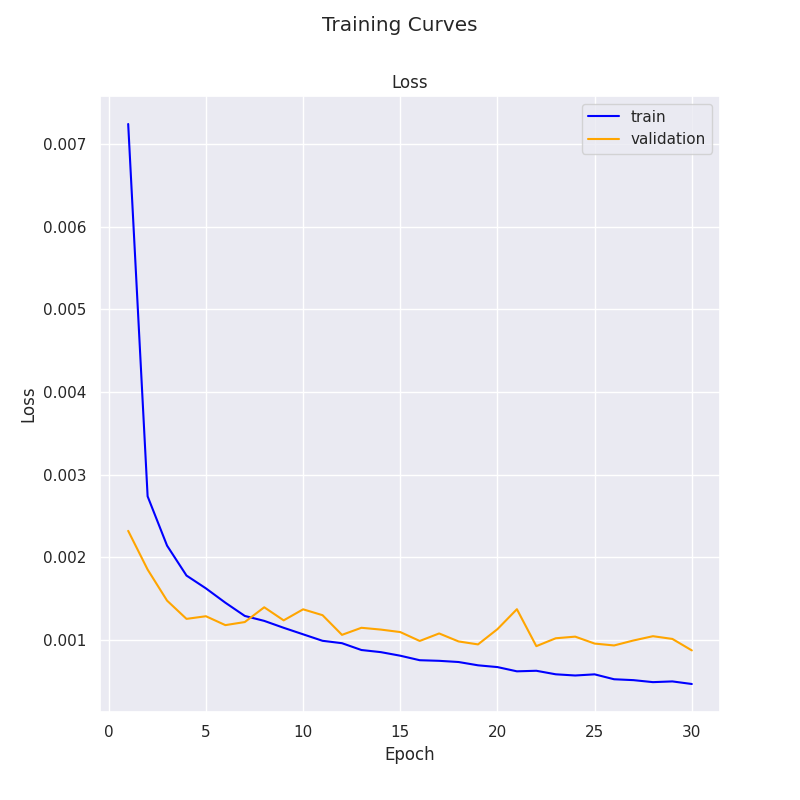
\includegraphics[width=0.8\textwidth]{images/chapter experiments/method 1/image 1/train_curve.png}
    \caption{Στο σχήμα παρατηρούμε τις γραφικές παραστάσεις του σφάλματος εκπαίδευσης και ελέγχου (\en{validation} ή \en{test}) κατά τη διάρκεια των 30 εποχών για το μοντέλο με την καλύτερη επίδοση στον πίνακα \ref{tab:method_1_hyperparameter_tuning_mnist_alg1}.}
    \label{fig:exp_method_1_mnist_alg1}
  \end{figure}
Στην εικόνα \ref{fig:exp_method_1_mnist_alg1} παρατίθεται το σφάλμα εκπαίδευσης (\en{training loss}) και επαλήθευσης (\en{validation loss}) για το μοντέλο με την καλύτερη επίδοση στον ανωτέρω πίνακα ($Bs = 64, lr = 0.0005, r = 3, Reconstruction = yes$). Παρατηρούμε ότι ακόμα και στην 30κοστή εποχή, το σφάλμα επαλήθευσης μειώνεται.\par

% Πες για τα πειράματα του επόμενου αλγορίθμου.
Ο επόμενος σε σειρά αλγόριθμος είναι ο \en{Argmax Scaled Routing}. Ο αλγόριθμος αυτός κάνει την υπόθεση ότι μια ψήφος είναι αρκετή για τη διαμόρφωση μιας κάψουλας γονέα. Συνεπώς, για τη διαμόρφωση ολόκληρου του επιπέδου \en{DigitCaps} αρκεί να επιλεγούν (με κριτήριο τα βάρη δρομολόγησης) τόσες ψήφοι εκπρόσωποι όσος είναι και ο αριθμός των κλάσεων. Στον πίνακα \ref{tab:method_1_hyperparameter_tuning_mnist_alg2} παρατίθενται τα αποτελέσματα των πειραμάτων. Προφανώς, η δοκιμασία για 1 επανάληψη αλγορίθμου δρομολόγησης δεν υπάρχει καθώς σε αυτή την περίπτωση, όλα τα βάρη δρομολόγησης είναι ίσα (λόγω αρχικοποίησης).

\begin{table}[h]
    \begin{center}
        \en{
        \begin{tabular}{c c c c c c}
            \toprule
            Experiment & Batch Size & Routing Iter. & Learning Rate & Recon. & Test Error (\%) \\ 
            \midrule
            \multirow{4}{*}{Batch Size} & 32 & 3 & 0.001 & no & 0.54 \\
            & 64 & 3 & 0.001 & no & 0.53 \\
            & 32 & 3 & 0.001 & yes & 0.52 \\
            & 64 & 3 & 0.001 & yes & 0.51 \\
            \midrule
            \multirow{4}{*}{Routing Iter.} & 64 & 2 & 0.001 & no & 0.53 \\
            & 64 & 2 & 0.001 & yes & \textbf{0.39} \\
            & 64 & 3 & 0.001 & no & 0.53 \\
            & 64 & 3 & 0.001 & yes & 0.51 \\
            \midrule
            \multirow{4}{*}{Learning Rate} & 64 & 3 & 0.0005 & yes & 0.45 \\
            & 64 & 3 & 0.001 & yes & 0.51 \\
            & 64 & 3 & 0.002 & yes & 0.57 \\
            & 64 & 3 & 0.01 & yes & 0.59 \\
            \bottomrule
            
        \end{tabular}
        }
    \end{center}
    \caption[]{\label{tab:method_1_hyperparameter_tuning_mnist_alg2}Πειράματα στο \en{MNIST} για την αναζήτηση υπερπαραμέτρων στον αλγόριθμο \en{Argmax Scaled Routing} (αλγόριθμος \ref{alg:dynam_argmax_scaled_routing}) για 30 εποχές.}
\end{table}

Από τα ανωτέρω πειράματα μπορούμε να εξάγουμε τα εξής συμπεράσματα:
\begin{enumerate}
    \item Σχετικά με το πρώτο πείραμα, αν και οι διαφορές δεν είναι μεγάλες, φαίνεται να βοηθάει η αύξηση του μεγέθους δέσμης και η προσθήκη αποκωδικοποιητή κατά την εκπαίδευση.
    \item Σε αντίθεση με τον κλασικό αλγόριθμο δυναμικής δρομολόγησης, ο βέλτιστος αριθμός επαναλήψεων είναι 2. Όπως αποδεικνύεται στα ειδικά πειράματα (ενότητα \ref{sec:method1_special_experiments}), όσο αυξάνονται οι επαναλήψεις τόσο τα βάρη δρομολόγησης λαμβάνουν ακραίες τιμές (είτε 0 αν δρομολογούν ψήφους σε κάψουλες γονείς που δεν ανήκουν στη σωστή κλάση είτε 1 για κάψουλες παιδιά που ανήκουν στη σωστή κλάση στόχο). Συνεπώς, στις πρώτες επαναλήψεις, μπορεί τα βάρη δρομολόγησης να μην έχουν κορεστεί σε ακραίες τιμές αλλά από νωρίς τα βάρη που αντιστοιχούν στη σωστή κλάση έχουν τις μεγαλύτερες τιμές (αποδεικνύεται στην ενότητα \ref{sec:method1_special_experiments}). Το γεγονός όμως ότι η αύξηση των επαναλήψεων προκαλεί μείωση της επίδοσης στον συγκεκριμένο αλγόριθμο μας προδιαθέτει ότι υπάρχουν πολλές περιπτώσεις σύγχυσης όπου ενώ έτεινε προς τη σωστή κλάση, σε αργότερη επανάληψη άλλαξαν ριζικά τα βάρη ευνοώντας κάποια λανθασμένη κλάση. Η συγκεκριμένη περίπτωση περιγράφεται έμπρακτα στο δεύτερο σχήμα του έργου \cite{hinton2018matrix}. Επίσης, είναι πιθανό να οφείλεται στο ότι υπάρχουν κάψουλες που έχουν παράξει ψήφους με μικρή συμφωνία για την κάψουλα πρόβλεψης. Κατά τον κορεσμό τους, αυτές θα αποκτήσουν βάρη δρομολόγησης ίσα με τη μονάδα προς άλλες κάψουλες.
    \item Σε αντιστοιχία με τις παραμέτρους της προηγούμενης μεθόδου, βλέπουμε ότι ένας χαμηλότερος ρυθμός μάθησης βοηθάει τη διαδικασία εκπαίδευσης.
\end{enumerate}
% image 2
\begin{figure}[h]
    \centering
    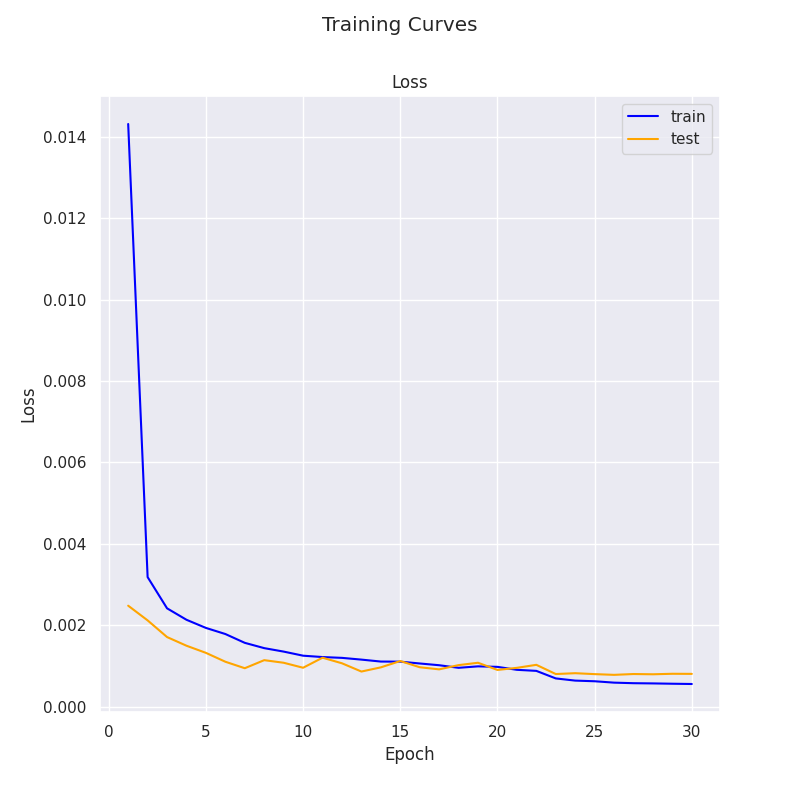
\includegraphics[width=0.8\textwidth]{images/chapter experiments/method 1/image 2/train_curve.png}
    \caption{Στο σχήμα παρατηρούμε τις γραφικές παραστάσεις του σφάλματος εκπαίδευσης και ελέγχου (\en{validation} ή \en{test}) κατά τη διάρκεια των 30 εποχών για το μοντέλο με την καλύτερη επίδοση στον πίνακα \ref{tab:method_1_hyperparameter_tuning_mnist_alg2}.}
    \label{fig:exp_method_1_mnist_alg2}
  \end{figure}
Στην εικόνα \ref{fig:exp_method_1_mnist_alg2} παρατίθεται το σφάλμα εκπαίδευσης (\en{training loss}) και επαλήθευσης (\en{validation loss}) για το μοντέλο με την καλύτερη επίδοση στον ανωτέρω πίνακα ($Bs = 64, lr = 0.001, r = 2, Reconstruction = yes$). Παρατηρούμε ότι ακόμα και στη 30κοστή εποχή, το σφάλμα επαλήθευσης μειώνεται.\par

% Πες για τα πειράματα του επόμενου αλγορίθμου.
Ο επόμενος σε σειρά αλγόριθμος είναι ο \en{Argmax Routing}. Και αυτός ο αλγόριθμος κάνει την υπόθεση ότι μια ψήφος είναι αρκετή για τη διαμόρφωση μιας κάψουλας γονέα. Συνεπώς, και πάλι, για τη διαμόρφωση ολόκληρου του επιπέδου \en{DigitCaps} αρκεί να επιλεγούν (με κριτήριο τα βάρη δρομολόγησης) τόσες ψήφοι εκπρόσωποι όσος είναι και ο αριθμός των κλάσεων. Υπενθυμίζεται ότι η διαφορά με τον \en{Argmax Scaled Routing} είναι ότι δεν πραγματοποιείται κλιμάκωση των εκπροσώπων με βάση το αντίστοιχο βάρος δρομολόγησης. Αυτό πάει ένα βήμα παραπέρα την υπόθεσή μας αφού πλέον, το μήκος των \en{DigitCaps} που καθορίζει την κλάση πρόβλεψης δεν εξαρτάται από το δυναμικό αλγόριθμο αλλά από τις επιλεγμένες ψήφους. Με απλά λόγια, ερχόμαστε ακόμα πιο κοντά στον ισχυρισμό ότι τα βάρη δρομολόγησης διαμορφώνονται αποκλειστικά από τις ψήφους με μεγάλο μέτρο (χωρίς να δίνεται ιδιαίτερη έμφαση στην πολυδιάστατη σύμπτωση).\par

Στον πίνακα \ref{tab:method_1_hyperparameter_tuning_mnist_alg3} παρατίθενται τα αποτελέσματα των σχετικών πειραμάτων. Προφανώς, όπως και στον προηγούμενο αλγόριθμο, η δοκιμασία για 1 επανάληψη αλγορίθμου δρομολόγησης δεν υπάρχει καθώς σε αυτή την περίπτωση, όλα τα βάρη δρομολόγησης είναι ίσα (λόγω αρχικοποίησης).

\begin{table}[h]
    \begin{center}
        \en{
        \begin{tabular}{c c c c c c}
            \toprule
            Experiment & Batch Size & Routing Iter. & Learning Rate & Recon. & Test Error (\%) \\ 
            \midrule
            \multirow{4}{*}{Batch Size} & 32 & 3 & 0.001 & no & 0.87 \\
            & 64 & 3 & 0.001 & no & \textbf{0.68} \\
            & 32 & 3 & 0.001 & yes & 0.90 \\
            & 64 & 3 & 0.001 & yes & 0.83 \\
            \midrule
            \multirow{4}{*}{Routing Iter.} & 64 & 2 & 0.001 & no & 0.88 \\
            & 64 & 2 & 0.001 & yes & 0.81 \\
            & 64 & 3 & 0.001 & no & 0.68 \\
            & 64 & 3 & 0.001 & yes & 0.83 \\
            \midrule
            \multirow{4}{*}{Learning Rate} & 64 & 3 & 0.0005 & yes & 0.99 \\
            & 64 & 3 & 0.001 & yes & 0.83 \\
            & 64 & 3 & 0.002 & yes & 0.75 \\
            & 64 & 3 & 0.01 & yes & 0.80 \\
            \bottomrule
            
        \end{tabular}
        }
    \end{center}
    \caption[]{\label{tab:method_1_hyperparameter_tuning_mnist_alg3}Πειράματα στο \en{MNIST} για την αναζήτηση υπερπαραμέτρων στον αλγόριθμο \en{Argmax Routing} (αλγόριθμος \ref{alg:dynam_argmax_routing}) για 30 εποχές.}
\end{table}

Από τα πειράματα του πίνακα μπορούμε να εξάγουμε τα εξής συμπεράσματα:
\begin{enumerate}
    \item Παρατηρούμε ότι η αύξηση του μεγέθους δέσμης συμβάλλει στην εκπαίδευση.
    \item Η αύξηση του ρυθμού επαναλήψεων βοηθάει στον συγκεκριμένο αλγόριθμο την επίδοση. Γεγονός που ενισχύει την τελευταία υπόθεση της αντίστοιχης παρατήρησης του προηγούμενου αλγορίθμου. Δηλαδή, το γεγονός ότι ο αλγόριθμος της μη κλιμάκωσης των ψήφων εκπροσώπων παρουσιάζει βελτίωση στις 3 επαναλήψεις συνεπάγεται ότι για κάθε κάψουλα γονέα επιλέγονται οι σωστές ψήφοι. Παρόλα αυτά, όταν τα βάρη δρομολόγησης φτάνουν στον κορεσμό, ίσως υπάρχουν και άλλες (λίγες) κάψουλες των οποίων οι ψήφοι δε συμφωνούν με τις άλλες ψήφους της σωστής κλάσης πρόβλεψης (π.χ. επειδή αναπαριστούν μέρη αντικειμένων που δεν εντοπίζονται στη συγκεκριμένη εικόνα εισόδου) αλλά τυχαίνει να συμφωνούν με λίγες ψήφους μιας άλλης κλάσης. Υπό αυτές τις συνθήκες, το αντίστοιχο βάρος δρομολόγησης της κάψουλας θα κορεστεί στη μονάδα πολύ γρήγορα\footnote{Στην ενότητα \ref{sec:method1_special_experiments} παρουσιάζεται μια τέτοια περίπτωση.}. 
    \item Σε αυτόν τον αλγόριθμο απαιτείται λίγο μεγαλύτερος ρυθμός μάθησης (ή περισσότερες εποχές).
\end{enumerate}
%% imaeg 3
\begin{figure}[h]
    \centering
    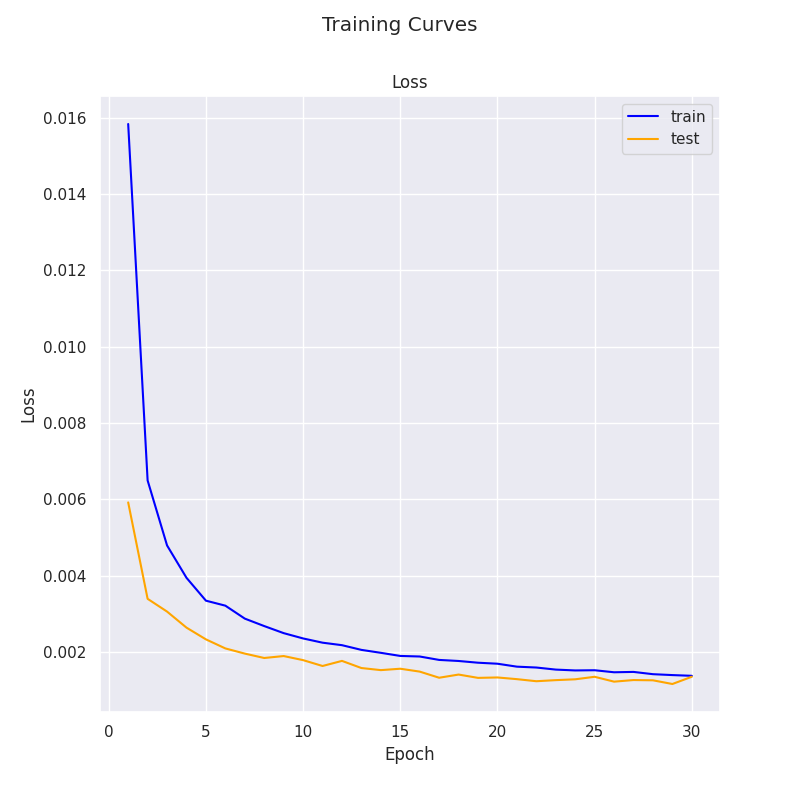
\includegraphics[width=0.8\textwidth]{images/chapter experiments/method 1/image 3/train_curve.png}
    \caption{Στο σχήμα παρατηρούμε τις γραφικές παραστάσεις του σφάλματος εκπαίδευσης και ελέγχου (\en{validation} ή \en{test}) κατά τη διάρκεια των 30 εποχών για το μοντέλο που ακολουθεί τον αλγόριθμο \en{Argmax Routing} που έχει τις υπερπαραμέτρους με την καλύτερη επίδοση, όπως φαίνεται στον πίνακα \ref{tab:method_1_hyperparameter_tuning_mnist_alg3}.}
    \label{fig:exp_method_1_mnist_alg3}
  \end{figure}
Στην εικόνα \ref{fig:exp_method_1_mnist_alg3} παρατίθεται το σφάλμα εκπαίδευσης (\en{training loss}) και επαλήθευσης (\en{validation loss}) για το μοντέλο με την καλύτερη επίδοση στον ανωτέρω πίνακα ($Bs = 64, lr = 0.001, r = 3, Reconstruction = no$). Παρατηρούμε ότι ακόμα και στη 30κοστή εποχή, το σφάλμα επαλήθευσης μειώνεται. Πιθανότατα, το γεγονός αυτό είναι η εξήγηση της αύξησης του σφάλματος με τη χρήση του αποκωδικοποιητή.\par

Σε κάθε διάταξη, η μέθοδος αυτή παρουσιάζει χειρότερα αποτελέσματα. Συνεπώς, απορρίπτονται οι υποθέσεις σχετικά με τη μη συνεισφορά των βαρών δρομολόγησης. Τέλος, το πόρισμα αυτό είναι ήδη αναμφίβολο (και λόγω παλαιότερων πειραμάτων σε 100 εποχές) και άρα, δεν έχει νόημα η δοκιμή του αλγορίθμου αυτού σε όλα τα σύνολα δεδομένων.\par

% Πες για τα πειράματα του επόμενου αλγορίθμου.
Ο τελευταίος αλγόριθμος που εξετάζουμε σε αυτή τη μέθοδο είναι ο \en{Max Routing}. Υπενθυμίζεται ότι ο αλγόριθμος αυτός απορρίπτει τελείως τον δυναμικό αλγόριθμο δρομολόγησης και μαζί του, την υπόθεση των νευρωνικών δικτύων από κάψουλες περί φιλτραρίσματος με πολυδιάστατη σύμπτωση. Υποστηρίζει ότι στον δυναμικό αλγόριθμο δρομολόγησης, η ψήφος (για κάθε \en{DigitCap}) με το μεγαλύτερο μέτρο διαδραματίζει τον μεγαλύτερο ρόλο στη διαμόρφωση του μέσου διανύσματος $s_j$ και με αυτόν τον τρόπο, απλά προσελκύει όσες ψήφους τυχαίνει να συμφωνούν μαζί της. Συνεπώς, υποστηρίζουμε με αυτή τη μέθοδο ότι δεν πρόκειται για ένα φιλτράρισμα συμφωνίας αλλά για μια αδικαιολόγητα περίπλοκη επιλογή μεγίστου διανύσματος.\par

Στον πίνακα \ref{tab:method_1_hyperparameter_tuning_mnist_alg4} παρατίθενται τα αποτελέσματα των σχετικών πειραμάτων. Προφανώς, η δοκιμασία για τον αριθμό των επαναλήψεων δεν έχει νόημα καθώς ο αλγόριθμος δεν είναι επαναληπτικός.

\begin{table}[h]
    \begin{center}
        \en{
        \begin{tabular}{c c c c c}
            \toprule
            Experiment & Batch Size & Learning Rate & Recon. & Test Error (\%) \\ 
            \midrule
            \multirow{4}{*}{Batch Size} & 32 & 0.001 & no & 0.92 \\
            & 64 & 0.001 & no & 0.81 \\
            & 32 & 0.001 & yes & \textbf{0.72} \\
            & 64 & 0.001 & yes & 0.89 \\
            \midrule
            \multirow{4}{*}{Learning Rate} & 64 & 0.0005 & yes & 1.00 \\
            & 64 & 0.001 & yes & 0.89 \\
            & 64 & 0.002 & yes & 0.90 \\
            & 64 & 0.01 & yes & 0.95 \\
            \bottomrule
            
        \end{tabular}
        }
    \end{center}
    \caption[]{\label{tab:method_1_hyperparameter_tuning_mnist_alg4}Πειράματα στο \en{MNIST} για την αναζήτηση υπερπαραμέτρων στον αλγόριθμο \en{Max Routing} (αλγόριθμος \ref{alg:dynam_max_routing}) για 30 εποχές.}
\end{table}

Από τα πειράματα του πίνακα μπορούμε να εξάγουμε τα εξής συμπεράσματα:
\begin{enumerate}
    \item Από τα αποτελέσματα, δεν μπορούμε να κρίνουμε ποια είναι η καλύτερη επιλογή μεγέθους δέσμης. Εκτιμούμε ότι σε αυτό τον αριθμό εποχών για τον συγκεκριμένο αλγόριθμο, μικρότερος αριθμός δέσμης είναι προτιμητέος.
    \item Σε αυτόν τον αλγόριθμο η τιμή $0.001$ για τον ρυθμό μάθησης φαίνεται να είναι ιδανική.
\end{enumerate}
%% image 4
\begin{figure}[h]
    \centering
    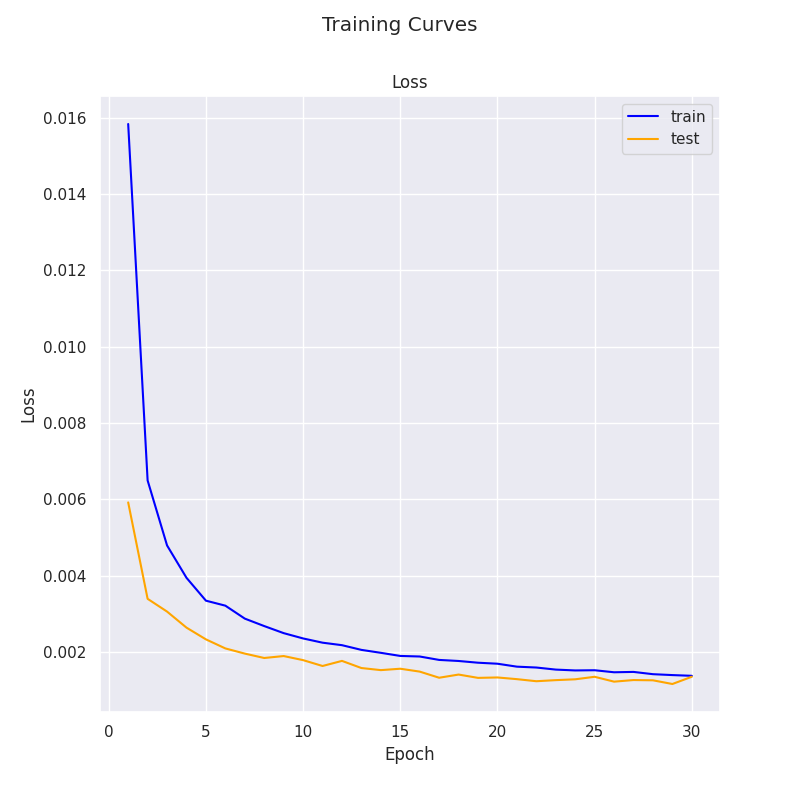
\includegraphics[width=0.8\textwidth]{images/chapter experiments/method 1/image 3/train_curve.png}
    \caption{Στο σχήμα απεικονίζονται οι γραφικές παραστάσεις του σφάλματος εκπαίδευσης και ελέγχου (\en{validation} ή \en{test}) κατά τη διάρκεια των 30 εποχών για το καλύτερο μοντέλο που ακολουθεί τον αλγόριθμο \en{Max Routing}, όπως προκύπτει από τον πίνακα \ref{tab:method_1_hyperparameter_tuning_mnist_alg4}.}
    \label{fig:exp_method_1_mnist_alg4}
  \end{figure}
Για άλλη μια φορά, στην εικόνα \ref{fig:exp_method_1_mnist_alg4} παρατίθεται το σφάλμα εκπαίδευσης (\en{training loss}) και επαλήθευσης (\en{validation loss}) για το μοντέλο με την καλύτερη επίδοση στον ανωτέρω πίνακα ($Bs = 32, lr = 0.001, Reconstruction = yes$). Παρατηρούμε ότι ακόμα και στη 30κοστή εποχή, το σφάλμα επαλήθευσης μειώνεται ακόμα.\par

Σε κάθε διάταξη, η μέθοδος αυτή παρουσιάζει χειρότερα αποτελέσματα σε σχέση με τις πρώτες δύο. Συνεπώς, αφενός δε θα γίνει εκτενή μελέτη αυτού σε όλα τα σύνολα δεδομένων και αφετέρου φαίνεται ότι ο αλγόριθμος δρομολόγησης πραγματικά συμβάλλει στην εκπαίδευση. Περισσότερα σχετικά πειράματα βρίσκονται στην ενότητα \ref{sec:method1_special_experiments}.

\subsubsection{Σύνολο Δεδομένων \en{CIFAR10}}
Αντίστοιχα με τα πειράματα για το σύνολο \en{MNIST}, παρατίθενται παρακάτω τα πειράματα για το πιο σύνθετο σύνολο δεδομένων \en{CIFAR10}. Οι λίγες εποχές που χρησιμοποιούνται για το συγκεκριμένο σύνολο σε συνδυασμό με την τάση των νευρωνικών δικτύων από κάψουλες να εξηγούν το οτιδήποτε βρίσκεται στην εικόνα (ακόμα και το παρασκήνιο) οδηγούν σε χαμηλές επιδόσεις. Σημειώνουμε ότι κατά αντιστοιχία με το έργο \cite{sabour2017dynamic}, χρησιμοποιήθηκε μια επιπλέον κλάση \en{none-of-the-above} για να δρομολογούν εκεί την ψήφο τους κάψουλες που αναπαριστούν αντικείμενα που δεν εμφανίζονται στην εικόνα. Επίσης, ο αριθμός των τύπων από κάψουλες αυξήθηκε από 32 σε 64 (όπως και στο έργο \cite{sabour2017dynamic}).\par

Ο αριθμός των πειραμάτων είναι μικρότερος από αυτόν για το σύνολο \en{MNIST}. Αυτό διότι, αν και το σύνολο \en{CIFAR10} έχει μεγάλη ετερογένεια με το προηγούμενο, ορισμένα πειράματα ποτέ δεν οδηγούν σε καλύτερα αποτελέσματα (ανεξαρτήτως συνόλου δεδομένων). Τα πειράματα αυτά έχουν αφαιρεθεί (όπως αυτό της δοκιμής του συνόλου δέσμης).

Τα πρώτα πειράματα για το σύνολο δεδομένων \en{CIFAR10} αφορούν τον κλασικό δυναμικό αλγόριθμο δρομολόγησης με συμφωνία (αλγόριθμος \ref{alg:dynam_routing}). Τα αποτελέσματα των πειραμάτων παρατίθενται στον πίνακα \ref{tab:method_1_hyperparameter_tuning_cifar10_alg1}.
\begin{table}[h]
    \begin{center}
        \en{
        \begin{tabular}{c c c c c c}
            \toprule
            Experiment & Batch Size & Routing Iter. & Learning Rate & Recon. & Test Error (\%) \\ 
            \midrule
            \multirow{2}{*}{Batch Size} & 32 & 3 & 0.0005 & yes & \textbf{20.60} \\
            & 64 & 3 & 0.0005 & yes & 23.96 \\
            \midrule
            \multirow{7}{*}{Routing Iter.} & 64 & 1 & 0.001 & no & 24.64 \\
            & 64 & 1 & 0.001 & yes & 23.19 \\
            & 64 & 2 & 0.001 & no & 29.25* \\
            & 64 & 2 & 0.001 & yes & 26.23* \\
            & 64 & 3 & 0.001 & no & 31.24* \\
            & 64 & 3 & 0.001 & yes & 29.15* \\
            \midrule
            \multirow{2}{*}{Learning Rate} & 64 & 3 & 0.0005 & yes & 23.96 \\
            & 64 & 3 & 0.001 & yes & 29.15* \\
            \bottomrule
            
        \end{tabular}
        }
    \end{center}
    \caption[]{\label{tab:method_1_hyperparameter_tuning_cifar10_alg1}Πειράματα στο \en{CIFAR10} για την αναζήτηση υπερπαραμέτρων στον αλγόριθμο δυναμικής δρομολόγησης με συμφωνία (αλγόριθμος \ref{alg:dynam_routing}) για 30 εποχές. Οι αριθμοί με αστερίσκο αναφέρονται σε περιπτώσεις αστάθειας του αλγορίθμου εκπαίδευσης.}
\end{table}

Από τα ανωτέρω πειράματα μπορούμε να εξάγουμε τα εξής συμπεράσματα:
\begin{itemize}
    \item Αναφορικά με το μέγεθος της δέσμης, παρατηρήθηκε ότι χαμηλότερο μέγεθος (32) εξαλείφει την όποια αστάθεια στον αλγόριθμο εκπαίδευσης. Για αυτό και η καλύτερη επίδοση επιτυγχάνεται με αυτό.
    \item Αναφορικά με τον αριθμό των επαναλήψεων, παρατηρούμε ότι η αύξησή τους επιδεινώνει την αστάθεια. Το γεγονός ότι οι καλύτερες παραμετροποιήσεις είναι για 3 επαναλήψεις σε συνδυασμό με τα πειράματα στο προηγούμενο σύνολο δεδομένων υποδεικνύουν ότι αυτή είναι η βέλτιστη υπερπαράμετρος.
    \item Για άλλη μια φορά, χαμηλότερη τιμή ρυθμού μάθησης βελτιώνει την επίδοση και μειώνει την πιθανότητα αστάθειας.
\end{itemize}


% Πες για τα πειράματα του επόμενου αλγορίθμου.
Ο επόμενος αλγόριθμος είναι ο \en{Argmax Scaled Routing}. Στον πίνακα \ref{tab:method_1_hyperparameter_tuning_cifar10_alg2} παρατίθενται τα αποτελέσματα των πειραμάτων. Να επαναλάβουμε ότι και για αυτό το σύνολο δεδομένων η δοκιμασία για 1 επανάληψη αλγορίθμου δρομολόγησης δεν υπάρχει καθώς σε αυτή την περίπτωση, όλα τα βάρη δρομολόγησης είναι ίσα (λόγω αρχικοποίησης).

\begin{table}[h]
    \begin{center}
        \en{
        \begin{tabular}{c c c c c c}
            \toprule
            Experiment & Batch Size & Routing Iter. & Learning Rate & Recon. & Test Error (\%) \\ 
            \midrule
            \multirow{4}{*}{Routing Iter.} & 64 & 2 & 0.001 & no & 28.10 \\
            & 64 & 2 & 0.001 & yes & \textbf{27.46} \\
            & 64 & 3 & 0.001 & no & 29.65 \\
            & 64 & 3 & 0.001 & yes & 31.02 \\
            \midrule
            \multirow{3}{*}{Learning Rate} & 64 & 3 & 0.0005 & yes & 29.06 \\
            & 64 & 3 & 0.001 & yes & 31.02 \\
            & 64 & 3 & 0.002 & yes & 31.60 \\
            \bottomrule
            
        \end{tabular}
        }
    \end{center}
    \caption[]{\label{tab:method_1_hyperparameter_tuning_cifar10_alg2}Πειράματα στο \en{CIFAR10} για την αναζήτηση υπερπαραμέτρων στον αλγόριθμο \en{Argmax Scaled Routing} (αλγόριθμος \ref{alg:dynam_argmax_scaled_routing}) για 30 εποχές.}
\end{table}

Τα ανωτέρω πειράματα, επιβεβαιώνουν τα συμπεράσματα των πειραμάτων στο σύνολο δεδομένων \en{MNIST}. Βλέπουμε ότι οι 2 επαναλήψεις είναι η βέλτιστη ρύθμιση για τον συγκεκριμένο αλγόριθμο ενώ επίσης, συνήθως βοηθάει η ελάττωση του ρυθμού μάθησης στην τιμή $0.0005$. Σημειώνουμε ότι ο αλγόριθμος αυτός (όπως και όλοι οι αλγόριθμοι εκτός του προηγούμενου), ουδέποτε εμφάνισε την οποιαδήποτε αστάθεια κατά την εκπαίδευση.


% Πες για τα πειράματα του επόμενου αλγορίθμου.
Ο επόμενος σε σειρά αλγόριθμος είναι όπως και πριν ο \en{Argmax Routing}. Στον πίνακα \ref{tab:method_1_hyperparameter_tuning_cifar10_alg3} παρατίθενται τα αποτελέσματα των σχετικών πειραμάτων (με τη δοκιμή για 1 επανάληψη να μην έχει ουσία).

\begin{table}[h]
    \begin{center}
        \en{
        \begin{tabular}{c c c c c c}
            \toprule
            Experiment & Batch Size & Routing Iter. & Learning Rate & Recon. & Test Error (\%) \\ 
            \midrule
            \multirow{4}{*}{Routing Iter.} & 64 & 2 & 0.001 & no & 38.96 \\
            & 64 & 2 & 0.001 & yes & 37.96 \\
            & 64 & 3 & 0.001 & no & 38.06 \\
            & 64 & 3 & 0.001 & yes & 38.49 \\
            \midrule
            \multirow{3}{*}{Learning Rate} & 64 & 3 & 0.0005 & yes & 38.97 \\
            & 64 & 3 & 0.001 & yes & 38.49 \\
            & 64 & 3 & 0.002 & yes & \textbf{37.83} \\
            \bottomrule
            
        \end{tabular}
        }
    \end{center}
    \caption[]{\label{tab:method_1_hyperparameter_tuning_cifar10_alg3}Πίνακας που περιέχει τα πειράματα που έγιναν στο σύνολο \en{CIFAR10} για την αναζήτηση υπερπαραμέτρων στον αλγόριθμο \en{Argmax Routing} (αλγόριθμος \ref{alg:dynam_argmax_routing}) για 30 εποχές.}
\end{table}

Για άλλη μια φορά επιβεβαιώνονται οι παρατηρήσεις που έγιναν στο σύνολο δεδομένων \en{MNIST} για τον αντίστοιχο αλγόριθμο. Φαίνεται ότι οι 3 επαναλήψεις οδηγούν σε καλύτερη επίδοση αφού σε αυτή τη ρύθμιση επιτυγχάνεται η καλύτερη επίδοση.

% Πες για τα πειράματα του επόμενου αλγορίθμου.
Κλείνοντας τα πειράματα για την εύρεση των βέλτιστων υπερπαραμέτρων, αναφέρουμε τα πειράματα που έγιναν στον αλγόριθμο \en{Max Routing} με το σύνολο δεδομένων \en{CIFAR10}. Στον πίνακα \ref{tab:method_1_hyperparameter_tuning_cifar10_alg4} παρατίθενται τα αποτελέσματα των σχετικών πειραμάτων. Προφανώς, όπως και στον προηγούμενο αλγόριθμο, η δοκιμασία για τον αριθμό των επαναλήψεων δεν έχει νόημα καθώς ο αλγόριθμος δεν είναι επαναληπτικός.

\begin{table}[h]
    \begin{center}
        \en{
        \begin{tabular}{c c c c c}
            \toprule
            Experiment & Batch Size & Learning Rate & Recon. & Test Error (\%) \\ 
            \midrule
            \multirow{3}{*}{Learning Rate} & 64 & 0.0005 & yes & \textbf{37.19} \\
            & 64 & 0.002 & yes & 37.60 \\
            \bottomrule
            
        \end{tabular}
        }
    \end{center}
    \caption[]{\label{tab:method_1_hyperparameter_tuning_cifar10_alg4}Πειράματα στο \en{CIFAR10} για την αναζήτηση υπερπαραμέτρων στον αλγόριθμο \en{Max Routing} (αλγόριθμος \ref{alg:dynam_max_routing}) για 30 εποχές.}
\end{table}

Από τα δύο περιάματα αποδεικνύεται ότι ο μικρότερος ρυθμός μάθησης βοηθάει γενικότερα στην εκπαίδευση των αλγορίθμων μας.


\subsection{Επιλεκτική Εμβάθυνση Πειραμάτων και Σύγκριση}
Για τους δύο αλγορίθμους της μεθόδου 1 με την καλύτερη επίδοση (αλγόριθμοι \ref{alg:dynam_routing} και \ref{alg:dynam_argmax_scaled_routing}) πραγματοποιήθηκαν εκτενέστερα πειράματα με περισσότερες εποχές, για όλα τα σύνολα δεδομένων και σε μεγαλύτερο μέγεθος δέσμης (εφόσον ήταν εφικτό). Τα νέα πειράματα αυτά, μαζί με τα παλαιότερα πειράματα από τις άλλες δύο μεθόδους (για 100 εποχές), τα παρουσιάζουμε συγκεντρωτικά στον πίνακα \ref{tab:method_1_all_datasets}.

\begin{table}[h]
    \begin{center}
        \en{
        \begin{tabular}{c c c c c c c}
            \toprule
            Dataset & Algorithm & Bs & r & Lr & Recon. & Test Error (\%) \\ 
            \midrule
            \multirow{8}{*}{MNIST} &Classic& 64 & 3 & 0.0005 & yes & 0.41 \\
            &Argmax Scaled& 64 & 2 & 0.0005 & yes & 0.43 \\
            &Classic& 128 & 3 & 0.0005 & yes & \textbf{0.31}* \\
            &Argmax Scaled& 128 & 2 & 0.001 & yes & 0.37* \\
            &Classic& 32 & 3 & 0.0005 & yes & 0.35 \\
            &Argmax Scaled& 32 & 2 & 0.001 & yes & 0.42 \\
            &Argmax& 64 & 3 & 0.001 & yes & 0.60 \\
            &Max& 32 & 0 & 0.001 & yes & 0.75 \\
            \midrule
            \multirow{2}{*}{FashionMNIST} &Classic& 64 & 3 & 0.0005 & yes & \textbf{6.94} \\
            &Argmax Scaled& 64 & 2 & 0.0005 & yes & 7.00 \\
            \midrule
            \multirow{2}{*}{CIFAR10} &Classic& 64 & 3 & 0.0005 & yes & \textbf{21.64} \\
            &Argmax Scaled& 64 & 2 & 0.0005 & yes & 22.16 \\
            \midrule
            \multirow{2}{*}{SmallNORB} &Classic& 64 & 3 & 0.0005 & yes & 17.01 \\
            &Argmax Scaled& 64 & 2 & 0.0005 & yes & \textbf{16.49} \\
            \bottomrule
            
        \end{tabular}
        }
    \end{center}
    \caption[]{\label{tab:method_1_all_datasets}Πίνακας που περιέχει τα πειράματα που έγιναν σε όλα τα σύνολα δεδομένων στους δύο αλγορίθμους με την καλύτερη επίδοση. Επίσης, περιέχονται για λόγoυς σύγκρισης ορισμένα πειράματα των δύο αλγορίθμων με τη λιγότερο καλή επίδοση (όπως μετρήθηκε στην προηγούμενη ενότητα). Σημειώνουμε ότι με τον όρο \en{Classic} αναφερόμαστε στον αλγόριθμο δυναμικής δρομολόγησης με συμφωνία. Επίσης, τα αποτελέσματα με αστερίσκο (*) προέκυψαν μετά από εκπαίδευση σε 150 εποχές.}
\end{table}
%% image 5 
\begin{figure}[h]
    \centering
    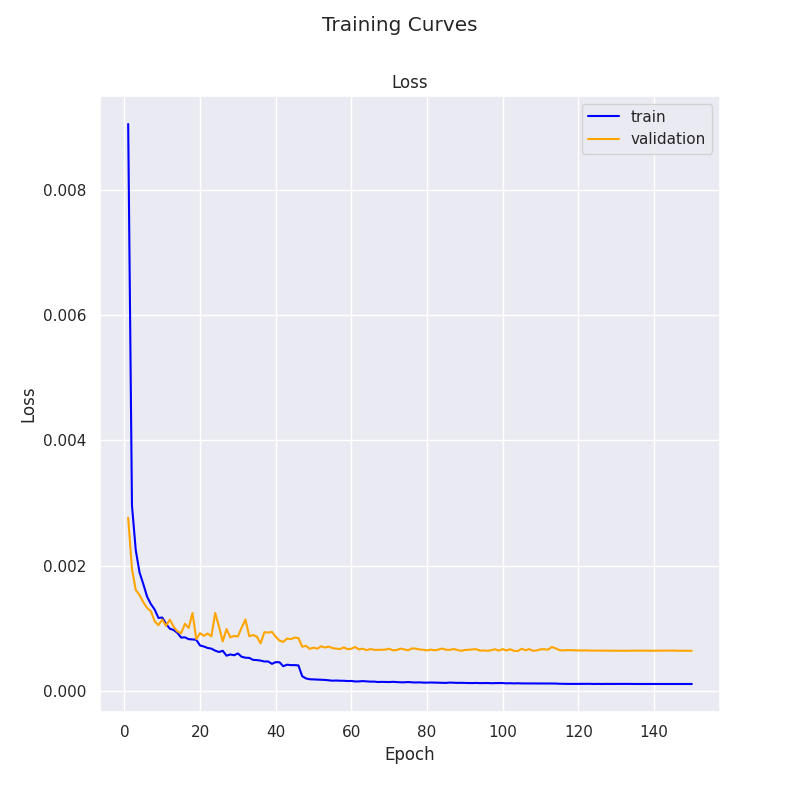
\includegraphics[width=0.8\textwidth]{images/chapter experiments/method 1/image 5/train_curve.png}
    \caption{Στο σχήμα παρατηρούμε τις γραφικές παραστάσεις του σφάλματος εκπαίδευσης και ελέγχου (\en{validation}) κατά τη διάρκεια των 150 εποχών για το μοντέλο που ακολουθεί τον αλγόριθμο \en{Dynamic Routing Between Capsules}. Είναι βέβαιο ότι παρατηρείται (\en{overfitting}) αλλά όχι σε βαθμό που να επηρεάζει την απόδοση στο σύνολο ελέγχου.}
    \label{fig:exp_method_1_best_alg}
  \end{figure}

Το πιο βέβαιο συμπέρασμα που μπορούμε να εξάγουμε από τα ανωτέρω αποτελέσματα είναι ότι ο αλγόριθμός μας \en{Argmax Scaled Routing} δεν παρουσιάζει έντονες διαφορές στην επίδοση σε σχέση με τον κλασικό αλγόριθμο δρομολόγησης με συμφωνία. Αν εξαιρέσουμε τα σύνολα δεδομένων \en{CIFAR10} και \en{SmallNORB} όπου ο αριθμός των εποχών δεν επαρκεί για τη σύγκλισή τους, στα υπόλοιπα σύνολα δεδομένων οι διαφορές στις επιδόσεις είναι μικρές.\par

Η παρόμοια ακρίβεια μεταξύ των δύο αλγορίθμων σημαίνει ότι η εξαγωγή ενός διανύσματος για κάθε κάψουλα \en{DigitCap} ως το σταθμισμένο άθροισμα των ψήφων δεν ωφελεί πρακτικά την επίδοση του δικτύου\footnote{Παρόλα αυτά, το σταθμισμένο άθροισμα μπορεί να ωφελεί τη σύλληψη των παραμέτρων στιγμιοτύπου της. Αυτό το διερευνούμε στην ενότητα \ref{sec:method1_special_experiments}}. Συνεπώς, τον πρωτεύοντα ρόλο τον έχουν τα βάρη δρομολόγησης που κλιμακώνουν τις ψήφους. Αυτά είναι ένα επαρκές κριτήριο για την επιλογή της ψήφου που θα δρομολογηθεί, κλιμακωμένη στο επόμενο επίπεδο. Το γεγονός αυτό μπορούμε να το εκμεταλλευτούμε μειώνοντάς τις επαναλήψεις και γλιτώνοντας υπολογιστικό κόστος. Αντί για τη μια περιττή επανάληψη θα μπορούσαμε να εισάγουμε ένα παραπάνω συνελικτικό επίπεδο που, όπως έχει αποδειχθεί στο κεφάλαιο \ref{chap:related_work}, βελτιώνει την ακρίβεια.\par 

Ένα ακόμα ερώτημα που προκύπτει φυσικά είναι αν το δίκτυο του αλγορίθμου \en{Argmax Scaled Routing} μαθαίνει τα βάρη του ώστε να ανταποκρίνεται με βέλτιστο τρόπο στον νέο μας αλγόριθμο ή αν εξαρχής ο κλασικός αλγόριθμος με συμφωνία έχει την ιδιότητα που περιγράφουμε (δηλαδή ότι το μέγιστο βάρος δρομολόγησης και η αντίστοιχη ψήφος - ψήφος \textquote{εκπρόσωπος} - αρκούν για τη δρομολόγηση). Το ερώτημα αυτό το απαντάμε στο \ref{sec:method1_special_experiments} ύστερα από τη διενέργεια κατάλληλων ειδικών πειραμάτων.\par

Ένα τελευταίο σημείο της σύγκρισης των δύο αλγορίθμων είναι ο χρόνος επίδοσης. Αναλυτικότερα, ο αλγόριθμος δυναμικής δρομολόγησης με συμφωνία (στον πίνακα αναγράφεται ως \en{Classic}), για μέγεθος δέσμης ίσο με 64 είναι κατά 3 δευτερόλεπτα πιο αργός από τον αλγόριθμο \en{Argmax Scaled Routing} (χρόνοι 33 και 30 δευτερόλεπτα αντίστοιχα). Σημειώνουμε ότι όλοι οι αλγόριθμοι έχουν ίσο αριθμό παραμέτρων, δηλαδή είναι $8,227k$ (οκτώ εκατομμύρια 227 χιλιάδες παράμετροι). Εξ' αυτών, οι $6,816k$ αφορούν τον κωδικοποιητή ενώ οι $1,411k$ τον αποκωδικοποιητή.\par  

Σε σύγκριση με τον απόλυτο αλγόριθμο \en{Max Rooting} της πρώτης μεθόδου, φαίνεται πως το φιλτράρισμα με πολυδιάστατη συμφωνία πραγματικά βοηθάει τις επιδόσεις του μοντέλου χωρίς να εισάγει επιπλέον παραμέτρους. Προφανώς λοιπόν, η υπόθεση ότι ο κλασικός αλγόριθμος δρομολόγησης μπορεί να μην προσφέρει κάτι παραπάνω από την απλή δρομολόγηση της μέγιστης σε μήκος ψήφου (για κάθε κάψουλα γονέα) είναι ορθή. Τέλος, σε σύγκριση με τον αλγόριθμο \en{Argmax Routing}, παρατηρούμε ότι υπάρχουν οφέλη από τη χρήση των βαρών δρομολόγησης όχι μόνο ως κριτήριο για την επιλογή των ψήφων εκπροσώπων αλλά ως μέγεθος για την επιλογή της κλάσης εξόδου (αφού διαμορφώνει άμεσα το μήκος των \en{DigitCaps}).

\section{Ειδικά Πειράματα Μεθόδου 1}
\label{sec:method1_special_experiments}
Στην ενότητα αυτή πραγματοποιούνται ειδικά πειράματα τα οποία στόχο έχουν να διαφωτίσουν την εσωτερική λειτουργία των νευρωνικών δικτύων με κάψουλες. Επίσης, στόχο έχουν να πιστοποιήσουν ότι οι προτεινόμενοι αλγόριθμοι πληρούν τις χαρακτηριστικές ιδιότητες της τεχνολογίας αλλά και να αποδείξουν ή να καταρρίψουν ορισμένες υποθέσεις αυτών. Τα πειράματα που παρουσιάζουμε αφορούν κυρίως το σύνολο δεδομένων \en{MNIST} αλλά παρόμοια συμπεράσματα (αν και λιγότερο προφανή) εξάγονται και για το σύνολο δεδομένων \en{Fashion-MNIST} που δοκιμάσαμε.

\subsection{Τι Μαθαίνει να Αναπαριστά η Κάθε Διάσταση του Διανύσματος \en{DigitCap}}
% Πειράματα ανακατασκευής
Ένα συνηθισμένο πείραμα της τεχνολογίας νευρωνικών δικτύων με κάψουλες είναι αυτό στο οποίο χρησιμοποιείται ο ανακατασκευαστής για να διαπιστωθεί τι αναπαριστά η κάθε διάσταση του διανύσματος \en{DigitCap}. Υπενθυμίζουμε ότι ένα από τα χαρακτηριστικά των νευρωνικών δικτύων είναι η δυνατότητα αποδόμησης του απεικονιζόμενου αντικειμένου και η ενθυλάκωση των παραμέτρων στιγμιοτύπου του στην αντίστοιχη ενεργή κάψουλα του τελευταίου επιπέδου. Παραδείγματα παραμέτρων στιγμιοτύπου είναι η πόζα, η φωτεινότητα αλλά και άλλα χαρακτηριστικά που αφορούν το συγκεκριμένο στιγμιότυπο. Στο πείραμα αυτό, χρησιμοποιώντας τον ανακατασκευαστή μπορούμε να έχουμε μια εικόνα του τι αναπαριστά το κάθε στοιχείο μιας κάψουλας τελευταίου επιπέδου.\par

Το συγκεκριμένο πείραμα ονομάζεται τυπικά πείραμα διαταραχής (\en{perturbation testing}). Πρακτικά, τροφοδοτούμε σε ένα εκπαιδευμένο - με τη χρήση αποκωδικοποιητή - μοντέλο νευρωνικού δικτύου από κάψουλες μια εικόνα και λαμβάνουμε το διάνυσμα της κάψουλας \en{DigitCap} με τη μεγαλύτερη τιμή ενεργοποίησης (με το μεγαλύτερο μήκος). Στη συνέχεια, μεταβάλουμε τις τιμές του διανύσματος (την κάθε μια ξεχωριστά) και τροφοδοτούμε το πειραγμένο διάνυσμα στον αποκωδικοποιητή. Παρατηρώντας την επίδραση των μεταβολών της κάψουλας στην ανακατασκευασμένη εικόνα, είμαστε σε θέση να  κατανοήσουμε το χαρακτηριστικό που η συγκεκριμένη θέση του διανύσματος \en{DigitCap} κωδικοποιεί. Προτού παρουσιάσουμε τα αποτελέσματα του πειράματος, σημειώνουμε ότι οι μεταβολές (\en{perturbations}) ανήκουν στο διάστημα $[-0.25, 0.25]$ και έχουν βήμα 0.05. Με αυτόν τον τρόπο, προκύπτει ότι για ένα διάνυσμα (κάψουλα) που έχει διάσταση 16, έχουμε 16 πειράματα για 11 μεταβολές.\par

% Σχήμα για το 4 perturbations new (image 6)
\begin{figure}[h]
    \centering
    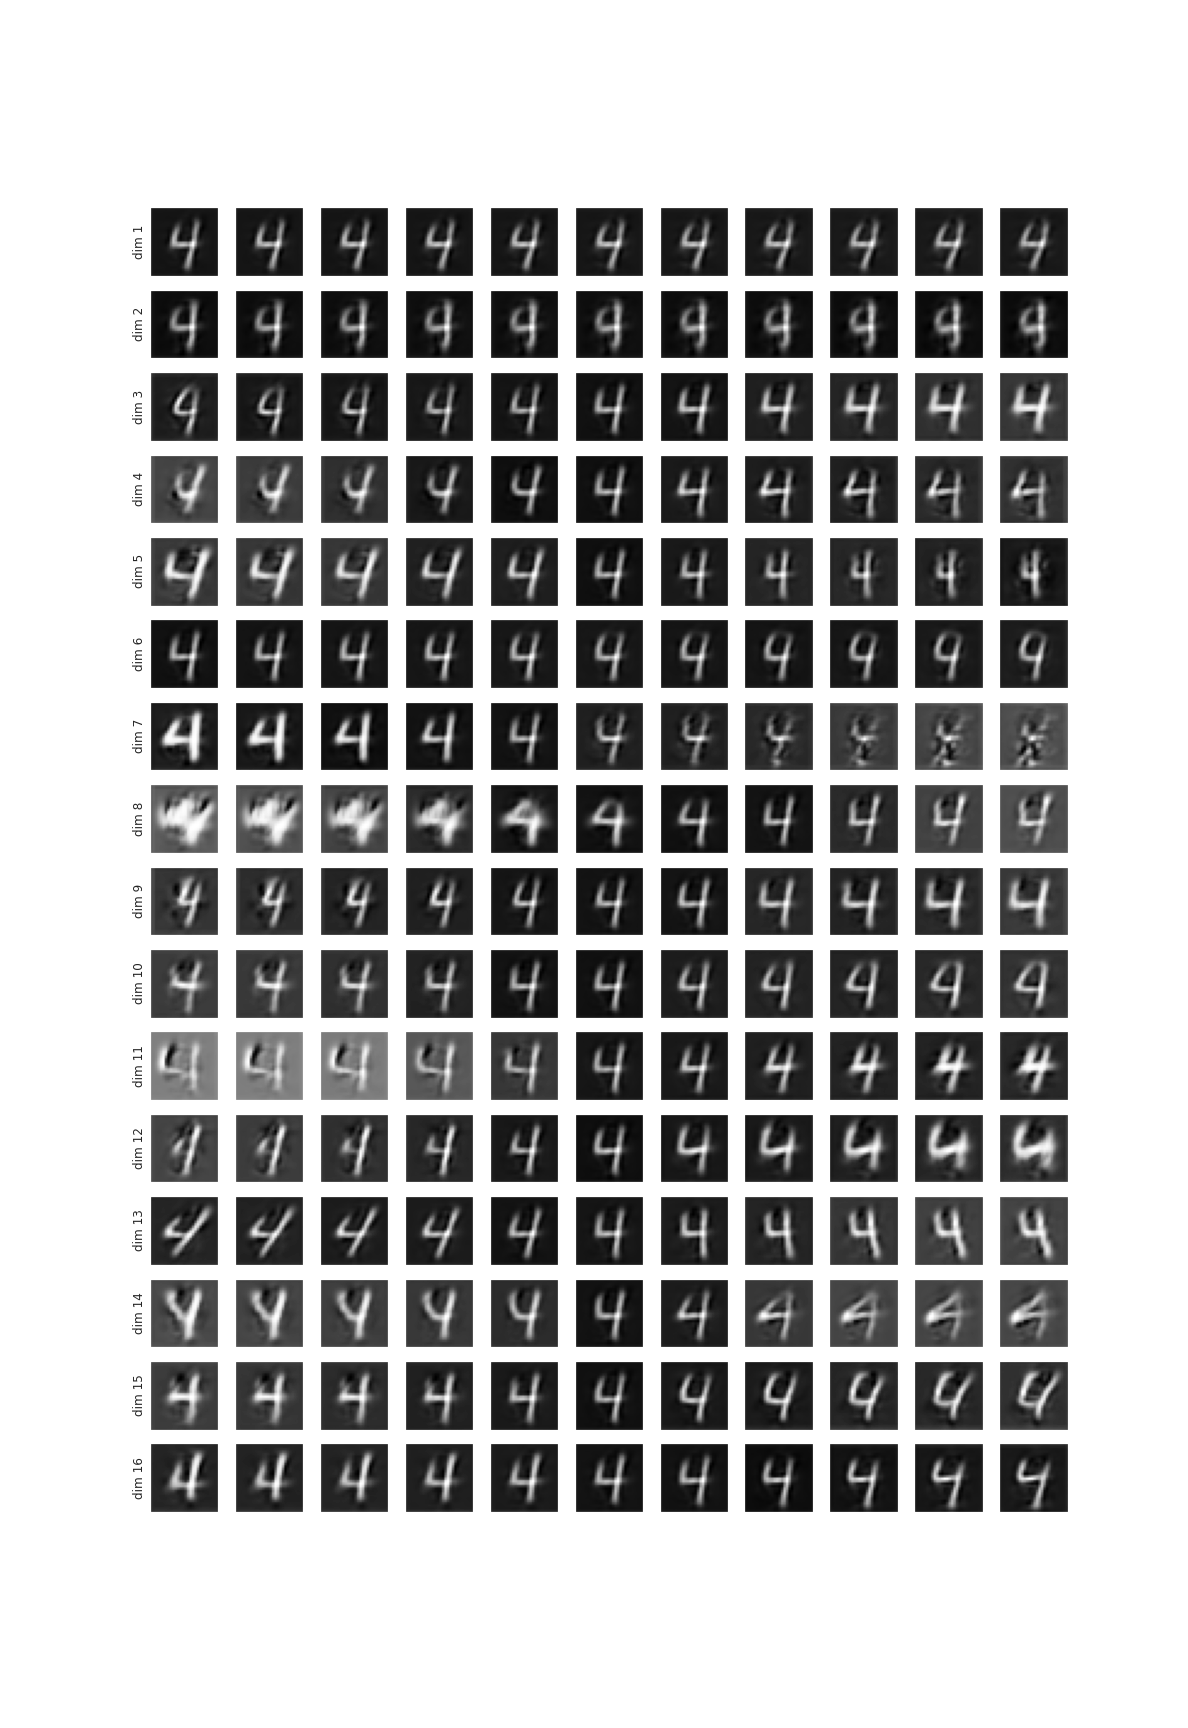
\includegraphics[width=0.7\textwidth]{images/chapter experiments/method 1/image 6/perturbations_19.png}
    \caption{\en{Perturbation tests} στο σύνολο δεδομένων \en{MNIST} στην κάψουλα \en{DigitCap} που αναπαριστά την κλάση 4 σε δίκτυο που εκπαιδεύτηκε με την χρήση του δυναμικού αλγορίθμου δρομολόγησης.}
    \label{fig:exp_method_1_special_perturb_1}
  \end{figure}

  % Σχήμα original vs output (image 6) 
\begin{figure}[h]
    \centering
    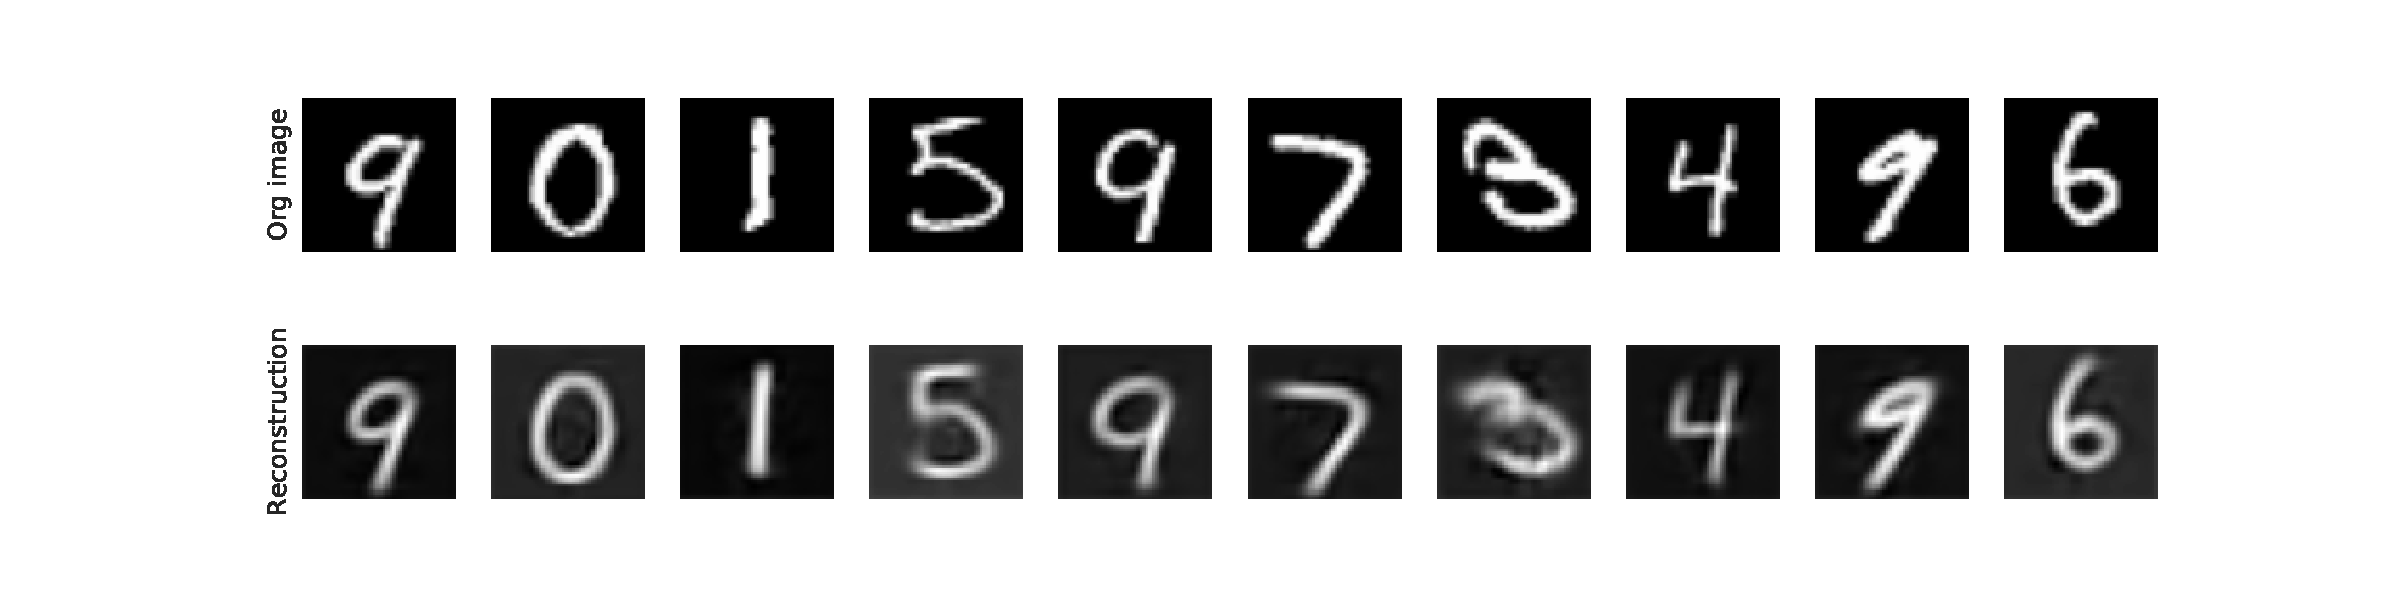
\includegraphics[width=0.7\textwidth]{images/chapter experiments/method 1/image 6/original_vs_reconstruction.pdf}
    \caption{Αντιπαραβολή της εικόνας εισόδου (πρώτη γραμμή) με την ανακατασκευασμένη εικόνα (δεύτερη γραμμή). Βλέπουμε ότι το δίκτυο μπορεί να λειτουργήσει ικανοποιητικά και ως αυτοκωδικοποιητής (\en{autoencoder}). Η θολούρα των εικόνων ανακατασκευής βελτιώνεται με την αύξηση των εποχών.}
    \label{fig:exp_method_1_special_perturb_many_1}
  \end{figure}

Στο σχήμα \ref{fig:exp_method_1_special_perturb_1} παρατίθενται τα αποτελέσματα του πειράματος για το σύνολο \en{MNIST} και για τον αλγόριθμο δυναμικής δρομολόγησης με συμφωνία. Αν και οι λίγες εποχές σε συνδυασμό με τον μικρό παράγοντα βαρύτητας του σφάλματος ανακατασκευής δεν έχουν επιτρέψει τον πλήρη σχηματισμό του αποκωδικοποιητή, είναι εμφανές ότι οι κάψουλες του τελευταίου επιπέδου (και συγκεκριμένα η κάψουλα 4 στο σχήμα) καταφέρνουν να συλλάβουν τις συγκεκριμένες παραμέτρους στιγμιοτύπου των απεικονιζόμενων αντικειμένων. Για παράδειγμα, για το ψηφίο 4, η 13\textsuperscript{η} διάσταση κωδικοποιεί τον προσανατολισμό του ψηφίου. Η 14\textsuperscript{η} την γωνία μεταξύ δύο ευθύγραμμων τμημάτων που συνθέτουν το ψηφίο 4 κ.ο.κ.\par


Αξίζει να σημειώσουμε ότι για κάθε κάψουλα, η κάθε διάσταση του διανύσματός της κωδικοποιεί διαφορετικές ιδιότητες του αντικειμένου που αναπαριστά. Παρόλα αυτά, ορισμένες διαστάσεις (π.χ. η δέκατη τρίτη) φαίνεται να έχουν καθολική ερμηνεία.\par

\begin{figure}[h]
    \centering
    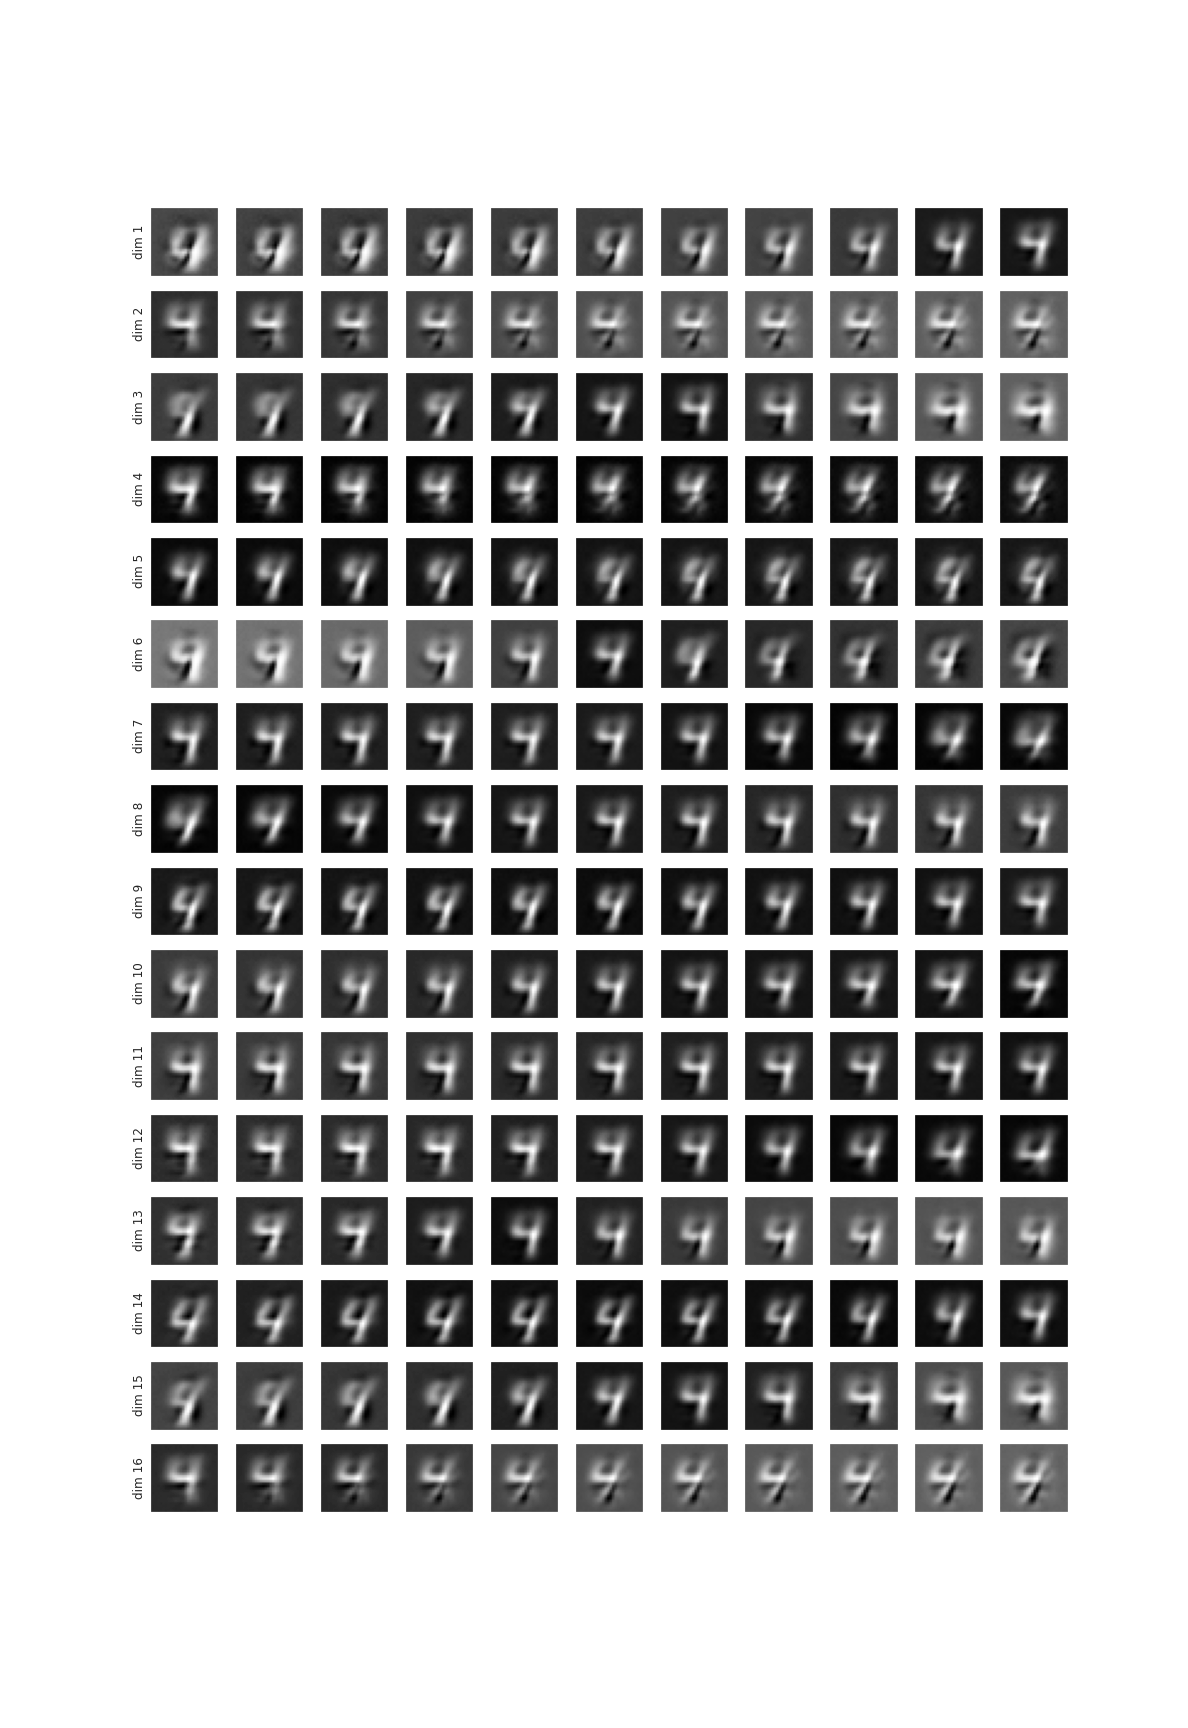
\includegraphics[width=0.8\textwidth]{images/chapter experiments/method 1/image 7/perturbations_19.png}
    \caption{\en{Perturbation tests} στο σύνολο δεδομένων \en{MNIST} στην κάψουλα \en{DigitCap} που αναπαριστά την κλάση 4 σε δίκτυο που εκπαιδεύτηκε με τη χρήση του αλγορίθμου \en{Argmax Scaled Routing}. Ενώ χρησιμοποιείται ο ίδιος αποκωδικοποιητής, το δίκτυο του κωδικοποιητή με τον συγκεκριμένο αλγόριθμο δρομολόγησης αδυνατεί να συλλάβει (\en{capture}) τις παραμέτρους στιγμιοτύπου των απεικονίσεων εισόδου.}
    \label{fig:exp_method_1_special_perturb_2}
  \end{figure}
%Σχήμα για το 4 από τον φάκελο perturbations argmax scaled (image 7)
Με μεγάλη περιέργεια πραγματοποιήσαμε τη συγκεκριμένη δοκιμασία για τους υπόλοιπους αλγορίθμους της μεθόδου 1. Αρχικά, για τον αλγόριθμο \en{Argmax Scaled Routing}, φαίνεται πως μετά από την εκπαίδευσή του στον ίδιο, περιορισμένο αριθμό εποχών με τον κλασικό αλγόριθμο, αδυνατεί σε μεγάλο βαθμό να συλλάβει τις ιδιότητες που αφορούν την αναπαράσταση των στιγμιοτύπων των αντικειμένων εισόδου (\en{equi\textendash variant parameters}). Για αυτό, στο σχήμα \ref{fig:exp_method_1_special_perturb_2} δε διακρίνεται έντονα κάποια γραμμή του οποίου τα στοιχεία να μεταβάλλονται κατά προβλέψιμο τρόπο.\par

Από αυτό το πείραμα μπορούμε να συμπεράνουμε ότι στην πραγματικότητα, το σταθμισμένο άθροισμα των ψήφων μπορεί να μην επηρεάζει σημαντικά την επίδοση αλλά διαδραματίζει καθοριστικό ρόλο στην ορθή λειτουργία των καψουλών. Φαίνεται ότι όλες μαζί οι συμφωνούντες ψήφοι συνθέτουν τις ιδιότητες του στιγμιοτύπου.\par

Η επίδοση στην παρούσα δοκιμασία γίνεται ακόμα πιο κακή καθώς απομακρυνόμαστε από τον κλασικό αλγόριθμο δρομολόγησης με συμφωνία. Στο σχήμα \ref{fig:exp_method_1_special_perturb_3} παρατίθεται το αποτέλεσμα της δοκιμασίας για τον αλγόριθμο \en{Max Routing}.\par

\begin{figure}[h]
    \centering
    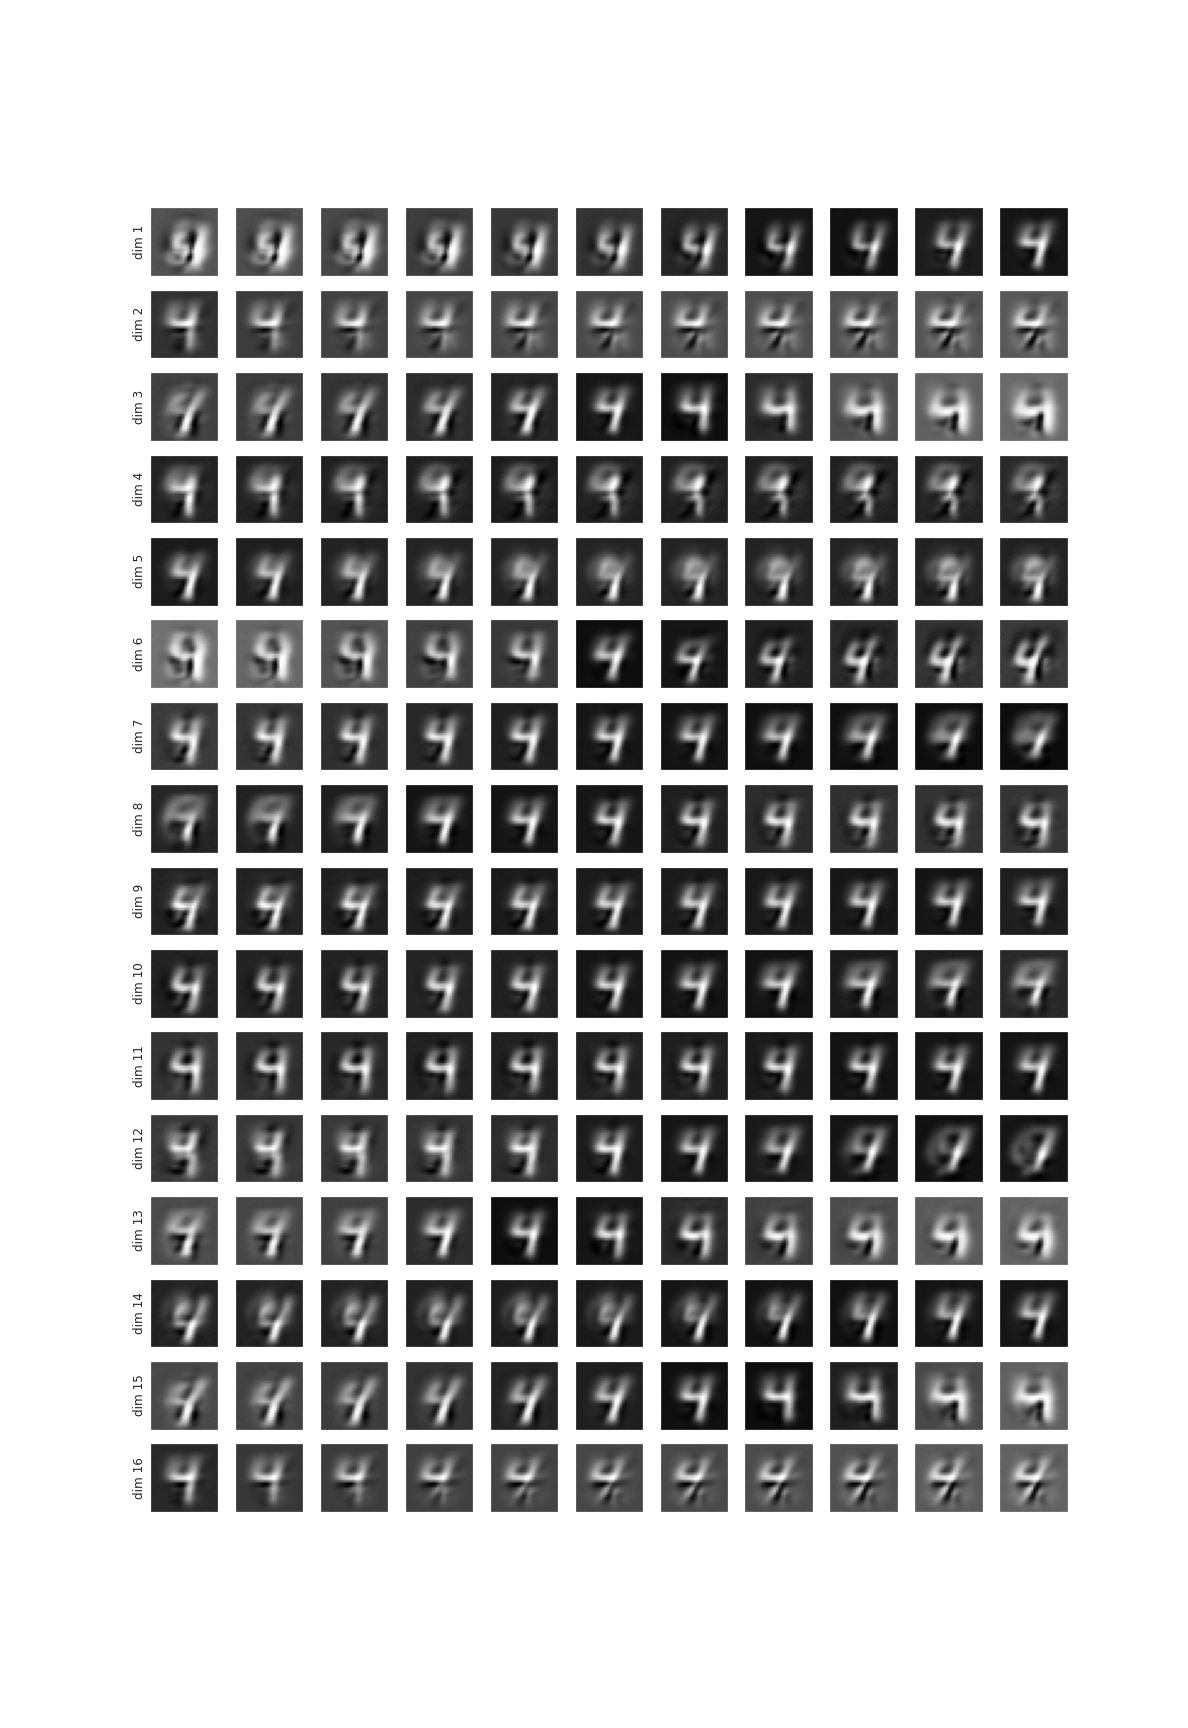
\includegraphics[width=0.8\textwidth]{images/chapter experiments/method 1/image 8/perturbations_19.png}
    \caption{\en{Perturbation tests} στο σύνολο δεδομένων \en{MNIST} στην κάψουλα \en{DigitCap} που αναπαριστά την κλάση 4 σε δίκτυο που εκπαιδεύτηκε με την χρήση του αλγορίθμου \en{Max Routing}. Η ανακατασκευή δεν είναι ακριβής λόγω της φύσης του αλγορίθμου δρομολόγησης που δεν παράγει \textquote{ισομεταβλητές} (\en{equi-variant}) αναπαραστάσεις.}
    \label{fig:exp_method_1_special_perturb_3}
  \end{figure}
% Σχήμα από φάκελο perturbations μαχ ροθτινγ (image 8)

Τέλος οδηγηθήκαμε σε μια μοναδική για την βιβλιογραφία δοκιμή εφαρμόζοντας το πείραμα στον κλασικό αλγόριθμο αλλά εκπαιδευμένο με το σύνολο δεδομένων \en{Fashion-MNIST}. Τα αποτελέσματα για τις περισσότερες διαστάσεις του διανύσματος της κάψουλας που αναπαριστά την κλάση υπόδημα δεν μπορούν να περιγραφούν με σαφή τρόπο. Παρόλα αυτά για ορισμένες διαστάσεις, οι μεταβολές είναι εμφανείς. Για παράδειγμα, στο σχήμα \ref{fig:exp_method_1_special_perturb_4} η διάσταση 6 κωδικοποιεί το ύψος του τακουνιού.
% Βάλε σχήμα από fashion mnist φάκελο (image 9)
\begin{figure}[h]
    \centering
    
\includegraphics[width=0.8\textwidth]{images/chapter experiments/method 1/image 9/perturbations_11_sixth_dim.png}
    \caption{\en{Perturbation tests} στο σύνολο δεδομένων \en{MNIST} στην έκτη διάσταση της κάψουλας \en{DigitCap} που αναπαριστά την κλάση \textquote{υπόδημα} σε δίκτυο που εκπαιδεύτηκε με την χρήση του αλγορίθμου \en{Classic Routing}. Στην εικόνα είναι εμφανές ότι η διάσταση αυτή κωδικοποιεί το ύψος του τακουνιού.}
    \label{fig:exp_method_1_special_perturb_4}
  \end{figure}

\subsection{Κριτήριο Επιλογής Ψήφων Αλγορίθμου Δυναμικής Δρομολόγησης με Συμφωνία}
% Εκπαίδευση στον κλασικό αλγόριθμο, δοκιμή στον αλγόριθμο max, argmax, argmax scaled.
% Το δίκτυο προσαρμόζεται στον νέο αλγόριθμο ή μαθαίνει έτσι και στην κλασική περίπτωση?

Οι αλγόριθμοι που παρουσιάσαμε στην μέθοδο 1 έχουν όλοι τους τον ίδιο αριθμό βαρών. Το μόνο που μεταβάλλεται είναι ο αλγόριθμος δρομολόγησης των ψήφων από το επίπεδο \en{PrimaryCaps} επίπεδο \en{DigitCaps}. Το γεγονός αυτό μας επιτρέπει την εφαρμογή των αλγορίθμων δρομολόγησης \ref{alg:dynam_argmax_scaled_routing}, \ref{alg:dynam_argmax_routing} και \ref{alg:dynam_max_routing} στο μοντέλο που έχει εκπαιδευτεί με την χρήση του αλγορίθμου \ref{alg:dynam_routing}. Κάθε μια από τις τρείς παραλλαγές του αλγορίθμου δρομολόγησης εξετάζει και ένα κριτήριο επιλογής εκπροσώπων. Θέλουμε να διαπιστώσουμε αν το κριτήριο αυτό είναι επαρκές για την δρομολόγηση των ψήφων ή όχι.\par

Πρακτικά, στο πείραμα αυτό χρησιμοποιούμε τα βάρη του μοντέλου που εκπαιδεύτηκε στο δυναμικό αλγόριθμο δρομολόγησης με συμφωνία και είχε την καλύτερη επίδοση ($0.31\%$ \en{Test Error}). Τα βάρη αυτά τα φορτώνουμε στα μοντέλα των τριών υπολοίπων αλγορίθμων και έπειτα εξετάζουμε τις επιδόσεις τους. Τα αποτελέσματα των πειραμάτων παρουσιάζονται στον πίνακα \ref{tab:special_experiments_algorithms_on_classic_model}. \par

\begin{table}[h]
    \begin{center}
        \en{
        \begin{tabular}{c c c c c}
            \toprule
            Trained on Algorithm & Tested on Algorithm & r & Total Loss & Test Error (\%)  \\ 
            \midrule
            \multirow{4}{*}{Dynamic Routing (Classic)} & Classic & 3 & 0.0007 & 0.31 \\
            & Argmax Scaled & 2 & 0.0064 & \textbf{0.30} \\
            & Argmax  & 3 & 0.0113 & 0.51 \\
            & Max & -1 & 2.6008 & 30.78 \\
            \bottomrule
            
        \end{tabular}
        }
    \end{center}
    \caption[]{\label{tab:special_experiments_algorithms_on_classic_model}Πειράματα στο \en{MNIST} με την εκπαίδευση του αλγορίθμου στον κλασικό, δυναμικό αλγόριθμο δρομολόγησης με συμφωνία και τον έλεγχο του μοντέλου αυτού με τη χρήση των τεσσάρων αλγορίθμων δρομολόγησης.}
\end{table}

Τα αποτελέσματα είναι τα αναμενόμενα για τους αλγορίθμους \en{Argmax} και \en{Max Routing}. Επίσης αναμενόμενες είναι όλες οι απώλειες (\en{Losses}) που προκύπτουν από το άθροισμα του σφάλματος περιθωρίου (\en{margin loss}) και του σφάλματος ανακατασκευής (\en{mean square error}). Άλλωστε, όπως διαπιστώσαμε στα πειράματα που προηγήθηκαν, ο κλασικός αλγόριθμος κάνει την καλύτερη ανακατασκευή αφού μόνο αυτός καταφέρνει να αποδομεί την εικόνα στις παραμέτρους στιγμιοτύπου (το επιτυγχάνει μέσα από την πράξη του σταθμισμένου αθροίσματος που δεν παρατηρείται στους άλλους αλγορίθμους).\par 

Το αξιοσημείωτο από τον πίνακα των αποτελεσμάτων είναι η επίδοση του αλγορίθμου \en{Argmax Scaled Routing} με βάρη που προέκυψαν από τον αλγόριθμο \en{Dynamic Routing} κατά την εκπαίδευσή του. Αν και η διαφορά είναι μικρή, το γεγονός αυτό συνεπάγεται ότι κατά την πρόβλεψη (\en{inference}) είναι προτιμότερο ένα κριτήριο επιλογής κάψουλας που θα δρομολογεί αυτή που αντιστοιχεί στο μέγιστο βάρος δρομολόγησης. Αυτό το γρήγορο κριτήριο οδηγεί σε καλύτερη επίδοση. Είναι λοιπόν προφανής ο ρόλος των βαρών δρομολόγησης στην επιλογή των κλάσεων. Αυτά εντοπίζουν την συμφωνία μεταξύ των ψήφων (που προκύπτουν από τα εκπαιδευμένα βάρη) και πριμοδοτούν την κλάση όπου υπάρχει μεγάλη συμφωνία με το να λαμβάνουν πολύ μεγάλη τιμή. Σε τελική ανάλυση, ο σημαντικός ρόλος των βαρών δρομολόγησης στην επιλογή της κλάσης προδίδεται από την χαμηλή επίδοση του αλγορίθμου \en{Argmax Routing} στον οποίο οι εκπρόσωποι δεν κλιμακώνονται από το αντίστοιχο βάρος δρομολόγησης.\par



\subsection{Συμφωνία Ψήφων}
% Πειράματα με confusion matrix
Στην ενότητα αυτή θέλουμε να εξετάσουμε την υπόθεση των νευρωνικών δικτύων με κάψουλες περί φιλτραρίσματος πολυδιάστατης σύμπτωσης. Αναλυτικότερα, χρησιμοποιούμε το καλύτερο μοντέλο μας που εκπαιδεύτηκε στον αλγόριθμο δυναμικής δρομολόγησης με συμφωνία και εξετάζουμε αν η κλάση πρόβλεψης είναι αυτή που εμφανίζει την μεγαλύτερη συμφωνία μεταξύ των ψήφων. Αν κάτι τέτοιο ισχύει, αποτελεί ακόμα μια επιβεβαίωση των θεμελιωδών υποθέσεων των νευρωνικών δικτύων με κάψουλες.\par

Αναλυτικότερα, για το πείραμά μας τροφοδοτούμε το μοντέλο με ένα παράδειγμα εισόδου της επιλογής μας και έπειτα συγκρίνουμε (με εσωτερικό γινόμενο) τις ψήφους που αντιστοιχούν στην κάθε κάψουλα γονέα μεταξύ τους. Έτσι, παράγεται ένας πίνακς προσοχής (\en{attention matrix}) για κάθε \en{DigitCap}. Έπειτα, λαμβάνουμε την μέση τιμή των στοιχείων του κάθε πίνακα προσοχής ξεχωριστά και έχουμε 10 ομοιότητες ψήφων: μια για κάθε κάψουλα γονέα. Σημειώνουμε ότι όλες τις ψήφους τις κλιμακώνουμε πριν υπολογίσουμε τα εσωτερικά γινόμενα ώστε να έχουν όλες μοναδιαίο μήκος.\par

Με μαθηματικούς όρους και χρησιμοποιώντας τον ενισχυμένο συμβολισμό (\en{notation}) του προηγούμενου κεφαλαίου έχουμε:
\begin{equation}
    \forall j \in \Omega_{L+1}: Similarity^L_{j} \gets \hat{V}^L_{j:} \times \hat{V}^{LΤ}_{j:}
\end{equation}
όπου το $\hat{V}^L$ συμβολίζει τις ψήφους αφότου (η κάθε μια) διαιρεθεί με την νόρμα της ώστε να έχει μοναδιαίο μήκος. Ισχύει $\hat{V}^L \in \Re^{ n^{L+1} \times n^L \times d^{L+1}}$.
% image 10
\begin{figure}[h]
    \centering
    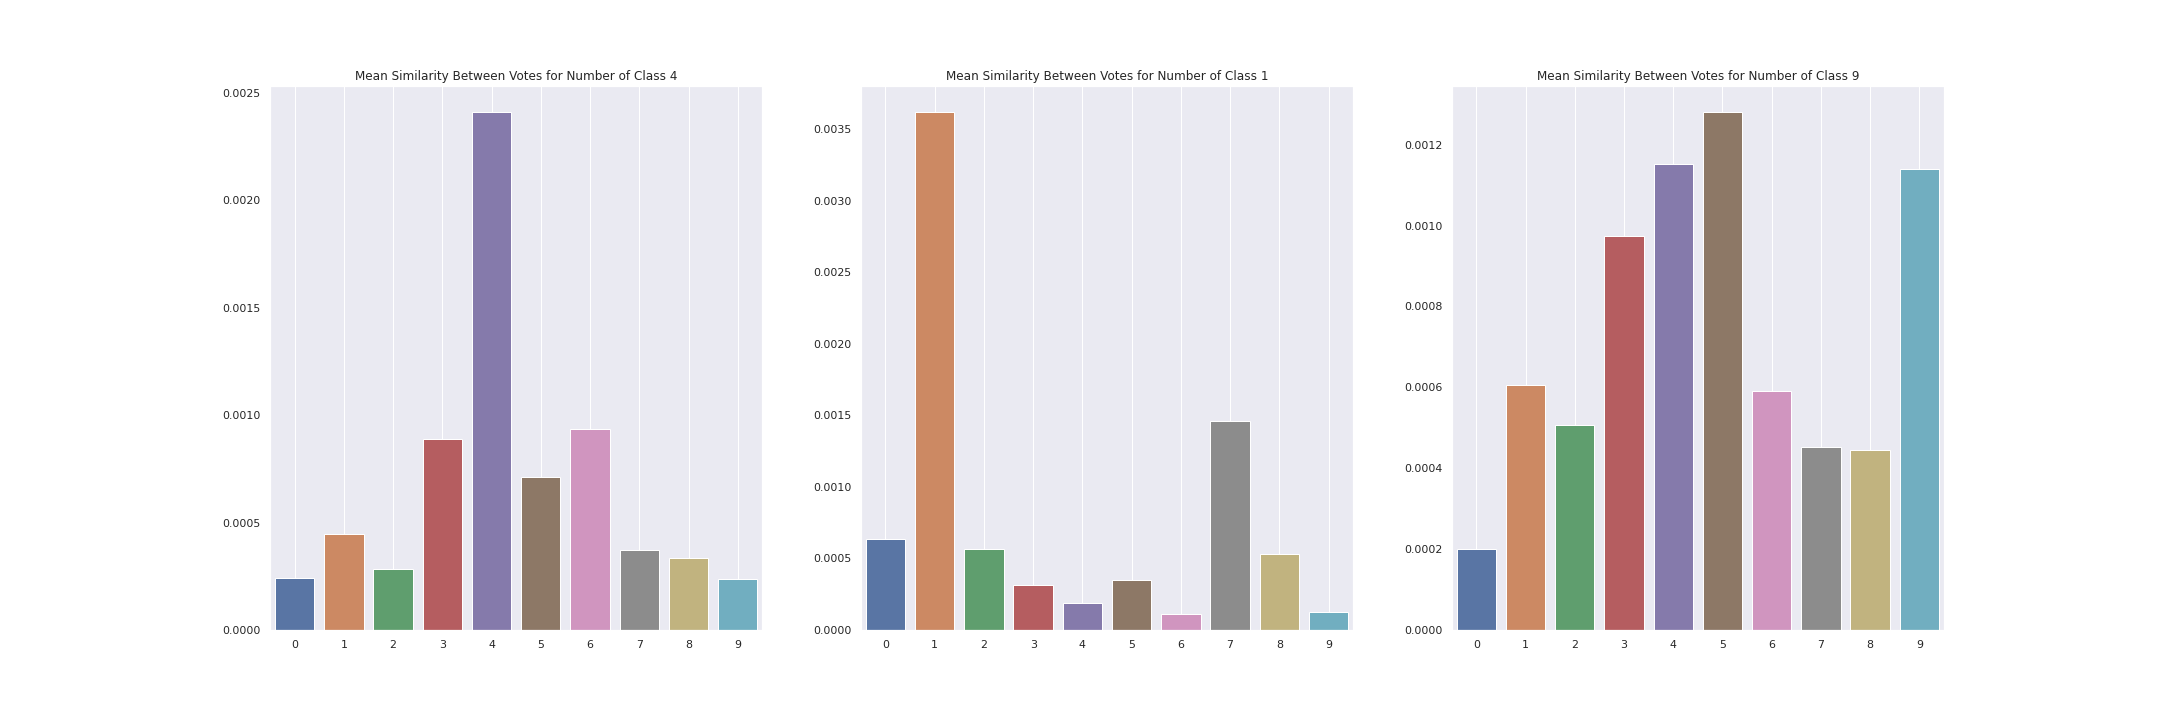
\includegraphics[trim={8cm 0 7.5cm 0},clip, width=0.98\textwidth]{images/chapter experiments/method 1/image 10/barplot_combined.png}
    \caption{Γραφικές παραστάσεις που απεικονίζουν την μέση συμφωνία ψήφων που έχουν προκύψει από τον αλγόριθμο δρομολόγησης με συμφωνία όταν αυτός τροφοδοτείται με εικόνες που περιέχουν τα νούμερα 4, 1 και 9 (από αριστερά προς τα δεξιά).}
    \label{fig:exp_method_1_special_vote_sim_1}
  \end{figure}

Από τα πειράματα αυτά, λαμβάνουμε τα αποτελέσματα που φαίνονται στην εικόνα \ref{fig:exp_method_1_special_vote_sim_1} παρατηρούμε ότι η συμφωνία παίζει καθοριστικό ρόλο στην δρομολόγηση των καψουλών αφού μέσω αυτής διαμορφώνονται τα βάρη δρομολόγησης. Στην εικόνα \ref{fig:exp_method_1_special_vote_sim_1}, στα δεξιά, συμπεριλαμβάνουμε και μια σπάνια περίπτωση όπου η μέση συμφωνία είναι μεγαλύτερη σε μη ορθή κλάση. Αυτό, όταν η διαφορά είναι μικρή, δεν οδηγεί απαραίτητα σε λανθασμένη πρόβλεψη (διότι έχουμε λάβει την μέση συμφωνία). Άλλωστε, για το σύνολο δεδομένω \en{Fashion-MNIST} στο οποίο δοκιμάσαμε και εκεί τα πειράματα, φάνηκε ότι στις περισσότερες περιπτώσεις, η μέση συμφωνία μεταξύ των ψήφων της κάψουλας που αντιστοιχεί στη σωστή πρόβλεψη δεν είναι η μεγαλύτερη\footnote{Αυτό είναι το πείραμα στο οποίο εμφανίστηκε η μεγαλύτερη διαφορά μεταξύ των δύο συνόλων δεδομένων. Στα υπόλοιπα πειράματα, τα συμπεράσματα είναι παρόμοια.}.\par
% image 11
\begin{figure}[h]
    \centering
    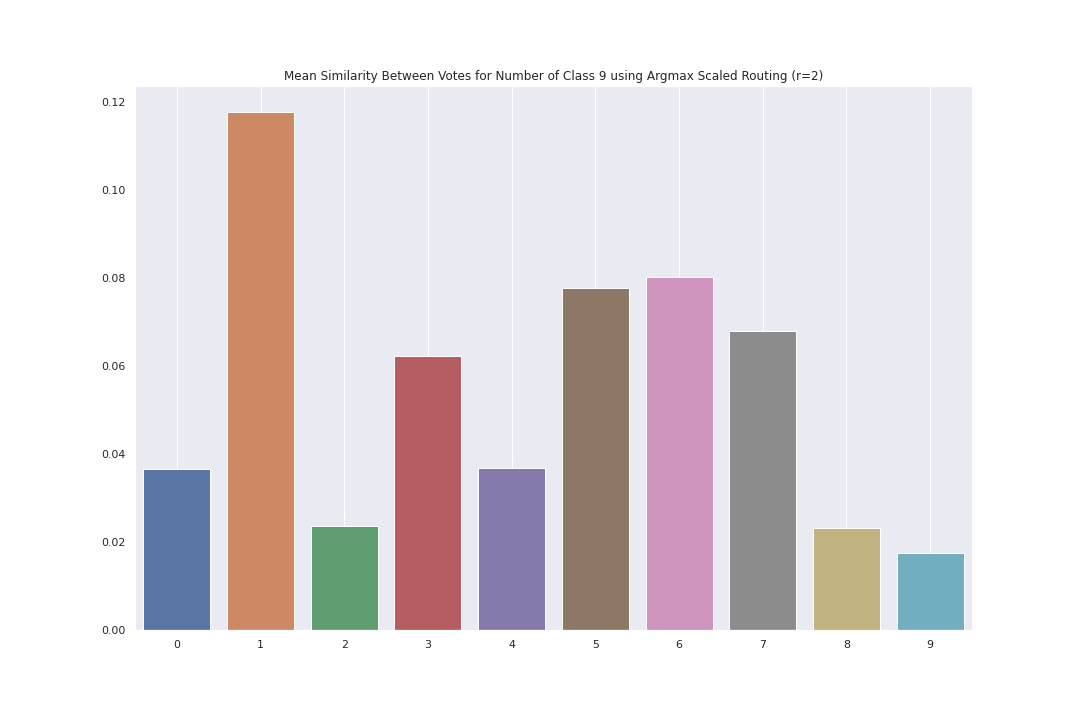
\includegraphics[ width=0.9\textwidth]{images/chapter experiments/method 1/image 11/barplot_number_9_batch_0.png}
    \caption{Γραφική παράσταση που απεικονίζει την μέση συμφωνία ψήφων που έχουν προκύψει από τον αλγόριθμο δρομολόγησης \en{Argmax Scaled Routing} όταν αυτός τροφοδοτείται με εικόνες που περιέχουν το νούμερο 9. Παρατηρούμε ότι η μέση συμφωνία της σωστής κλάσης είναι η πιο χαμηλή.}
    \label{fig:exp_method_1_special_vote_sim_2}
  \end{figure}
Δοκιμάσαμε το ίδιο πείραμα και σε μοντέλο εκπαιδευμένο στον αλγόριθμο \en{Argmax Routing} (βλέπε σχήμα \ref{fig:exp_method_1_special_vote_sim_2}). Όπως είναι αναμενόμενο, ο αλγόριθμος αδυνατώντας να αποδομήσει αποδοτικά την εικόνα, παράγει ψήφους που δεν έχουν μεγάλη μέση συμφωνία μεταξύ τους. Μάλιστα, φαίνεται στις περισσότερες περιπτώσεις να ισχύει το ανάποδο: δηλαδή η κλάση με την μικρότερη μέση συμφωνία φένεται να είναι η σωστή\footnote{Παραπέμπουμε τον αναγνώστη στην ιστοσελίδα του κώδικα για περισσότερα αποτελέσματα.}. Από άλλα πειράματα που δεν περιλαμβάνονται προέκυψε ότι ο συγκεκριμένος αλγόριθμος προτιμά να παράγει ψήφους για την σωστή κλάση όπου οι περισσότερες να μην εμφανίζουν υψηλή συμφωνία (εξού και η χαμηλή τιμή μέσης συμφωνίας). Αντίθετα, προτιμά, μεταξύ των ψήφων που προορίζονται για την σωστή κλάση να υπάρχουν ελάχιστες με την μέγιστη δυνατή συμφωνία (ώστε να \textquote{κερδίσουν} το ένα και μεγαλύτερο βάρος δρομολόγησης). Φυσικά, κάτι τέτοιο είναι απολύτως λογικό αφού μια είναι η ψήφος που θα προωθηθεί στο επόμενο επίπεδο. Από την στιγμή που δεν λαμβάνεται σαν αποτέλεσμα το σταθμισμένο άθροισμα και δεν υπάρχει φόβος τα διανύσματα να ακυρώσουν το ένα το άλλο (\en{cancel each other out}) δεν αποτελεί πρόβλημα η μικρή μέση συμφωνία.\par

\subsection{Κατανομή των Ψήφων}
% Πειράματα με τα γραφήματα με τις μπάρες.
Συνεχίζοντας τα ειδικά πειράματα, θα θέλαμε να διερευνύσουμε την υπόθεση σύμφωνα με την οποία, ο δυναμικός αλγόριθμος δρομολόγησης μπορεί να εκφυλιστεί στην επιλογή της μέγιστης σε μήκος ψήφου. Ισοδύναμα, θέλουμε να ελέγξουμε αν το μοντέλο διαμορφώνει τέτοια εκπαιδευόμενα βάρη ώστε να μη διαδραματίζει τόσο σημαντικό ρόλο η συμφωνία μεταξύ των ψήφων όσο το μήκος των ψήφων.\par

Από την μειωμένη επίδοση του αλγορίθμου \en{Max Routing}, ακόμα και όταν για την εκπαίδευση έχει χρησιμοποιηθεί ο αλγόριθμος \en{Classic Routing}, είμαστε προδιατεθειμένοι να πιστέψουμε ότι ο ανωτέρω ισχυρισμός δεν ευσταθεί. Πράγματι, τα πειράματα που διενεργούνται σε αυτή τη παράγραφο επιβεβαιώνουν την προδιάθεσή μας.\par
% image 12
% \begin{figure}[h]
%     \centering
%     \begin{minipage}{0.45\textwidth}
%     \centering
%     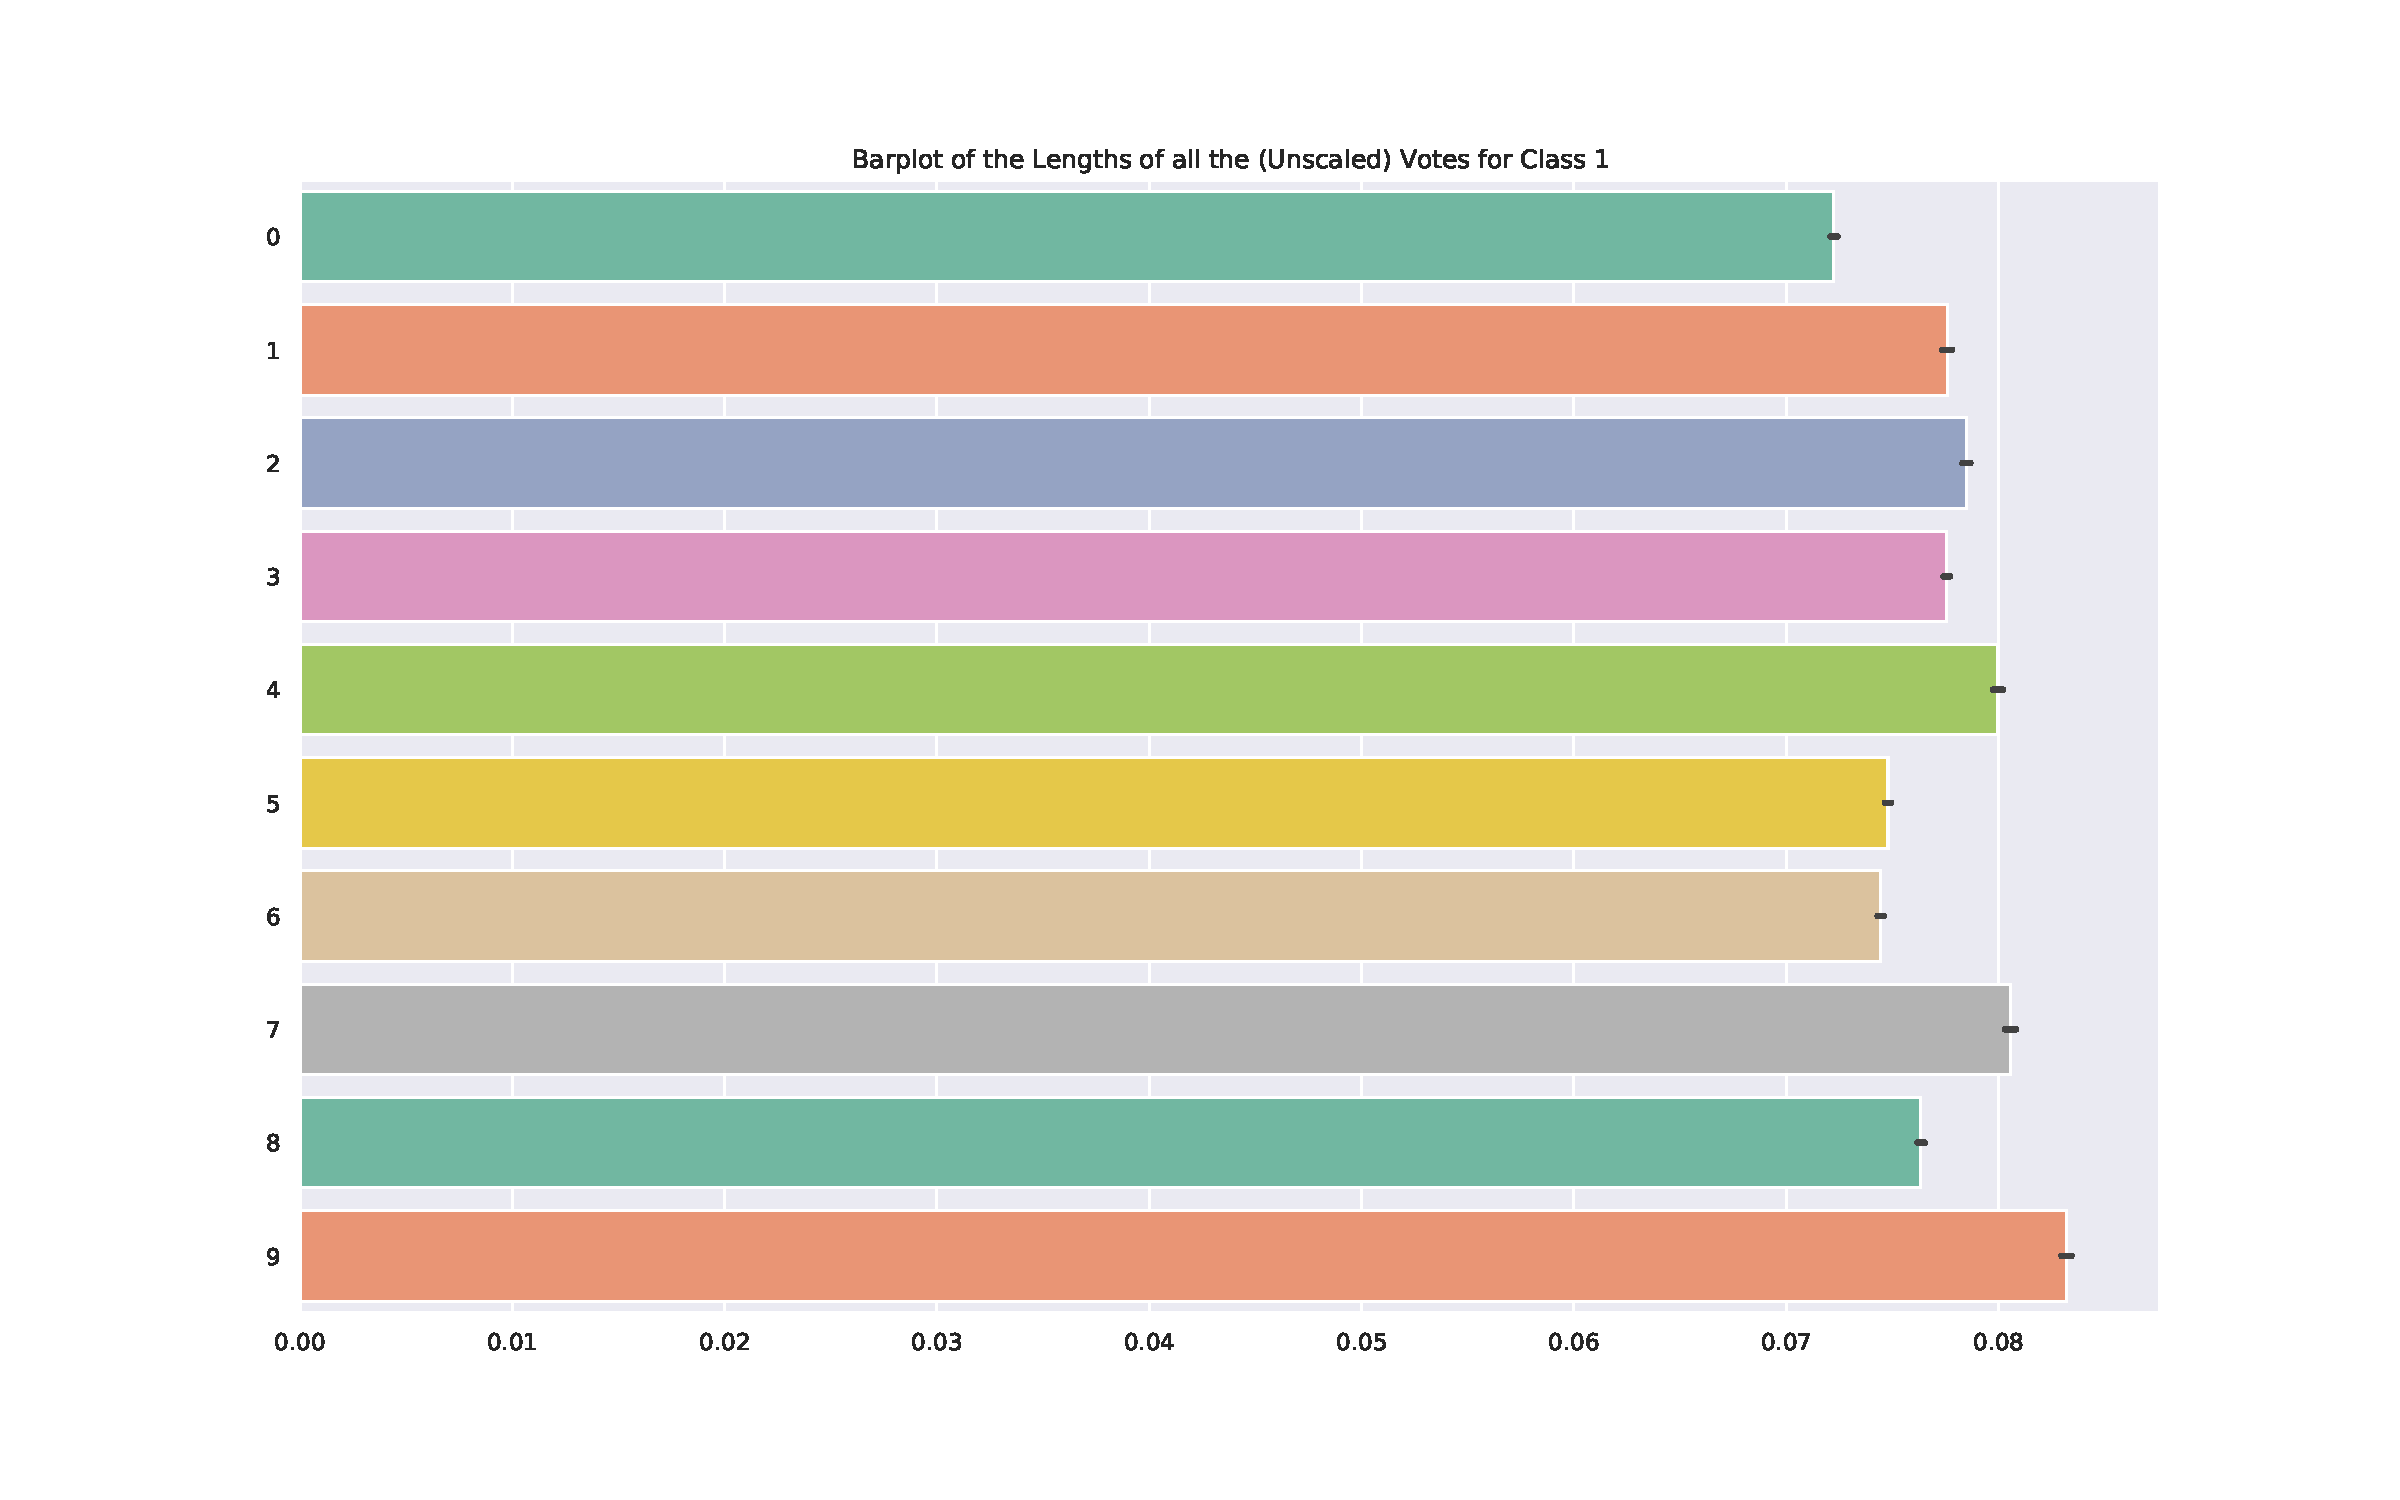
\includegraphics[width=0.3\linewidth, height=0.15\textheight]{images/chapter experiments/method 1/image 12/barplot_for_class_1_unscaled_True.pdf}
%     \caption{Γραφική παράσταση του μέσου μήκους των ψήφων ανά κλάση.}
%     \label{fig:exp_method_1_special_vote_dist_1}
%     \end{minipage}
    
%     \begin{minipage}{0.45\textwidth}
%     \centering
%     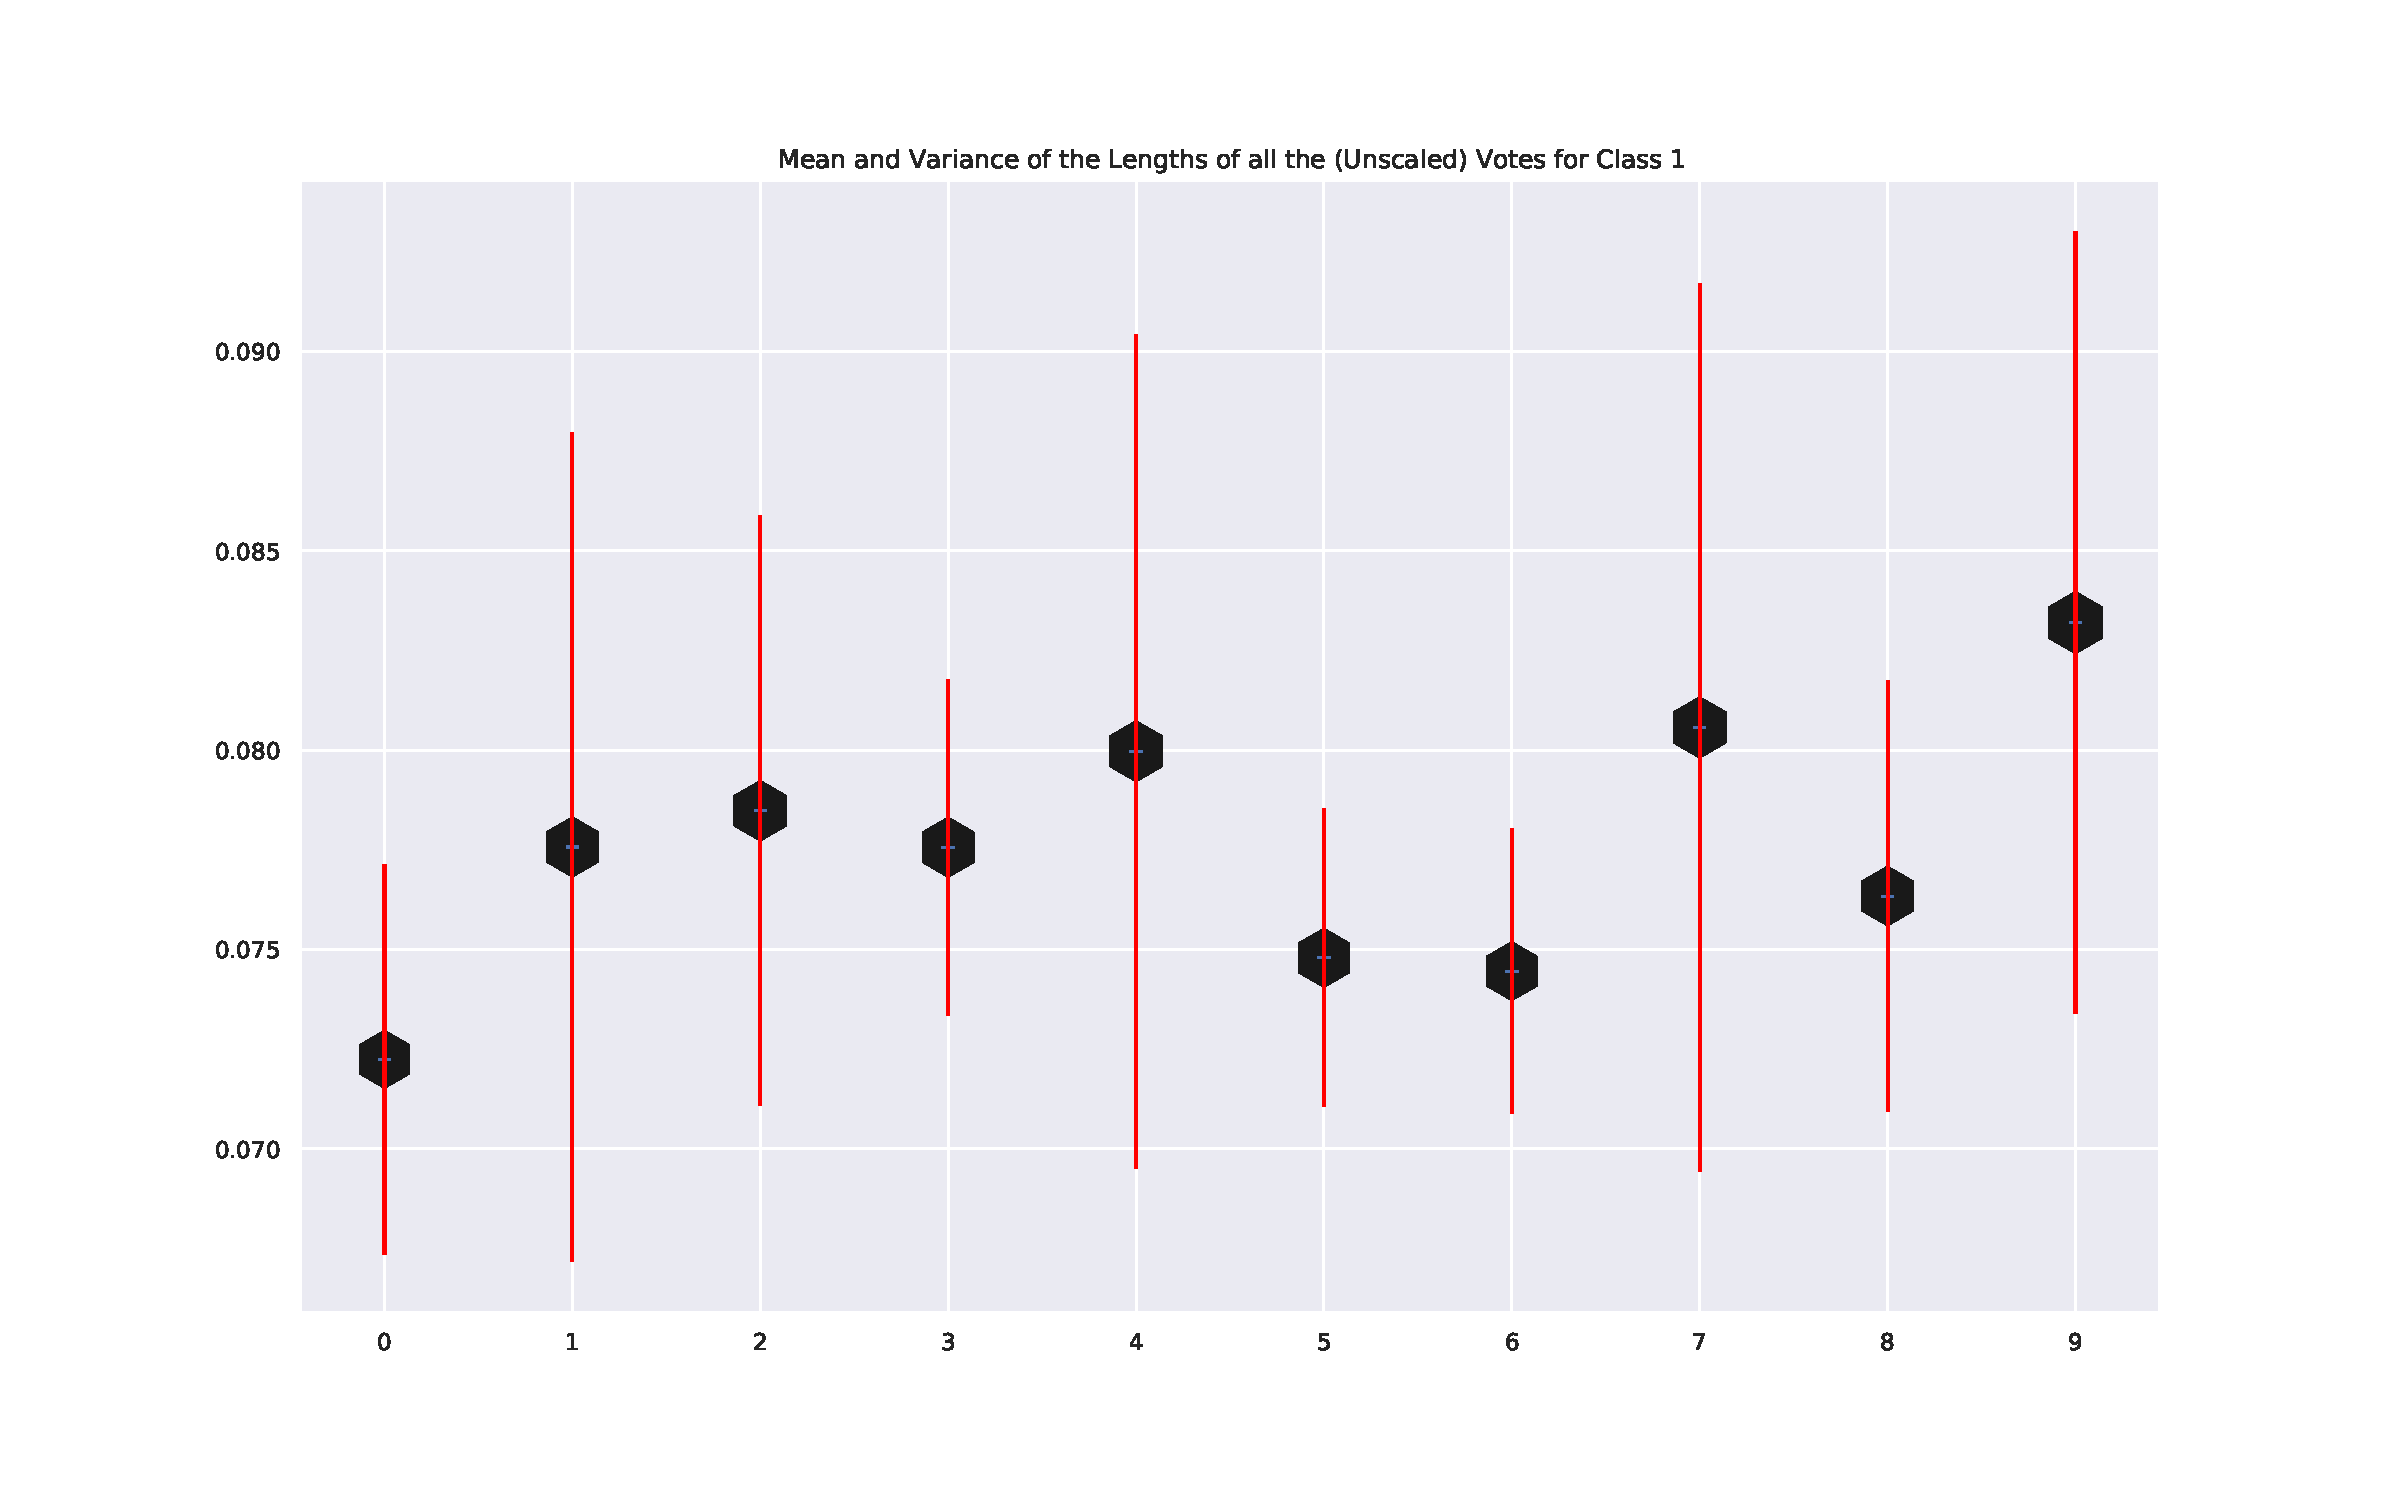
\includegraphics[width=0.3\linewidth, height=0.15\textheight]{images/chapter experiments/method 1/image 12/mean_var_for_class_1_unscaled_True.pdf}
%     \caption{Γραφική παράσταση του μέσου μήκους των ψήφων ανά κλάση. Στο διάγραμμα εμφανίζεται και η διασπορά με κόκκινες, κάθετες γραμμές.}
%     \label{fig:exp_method_1_special_vote_dist_2}
%     \end{minipage}
    
%   \end{figure}
\begin{figure}[h]
    \centering
    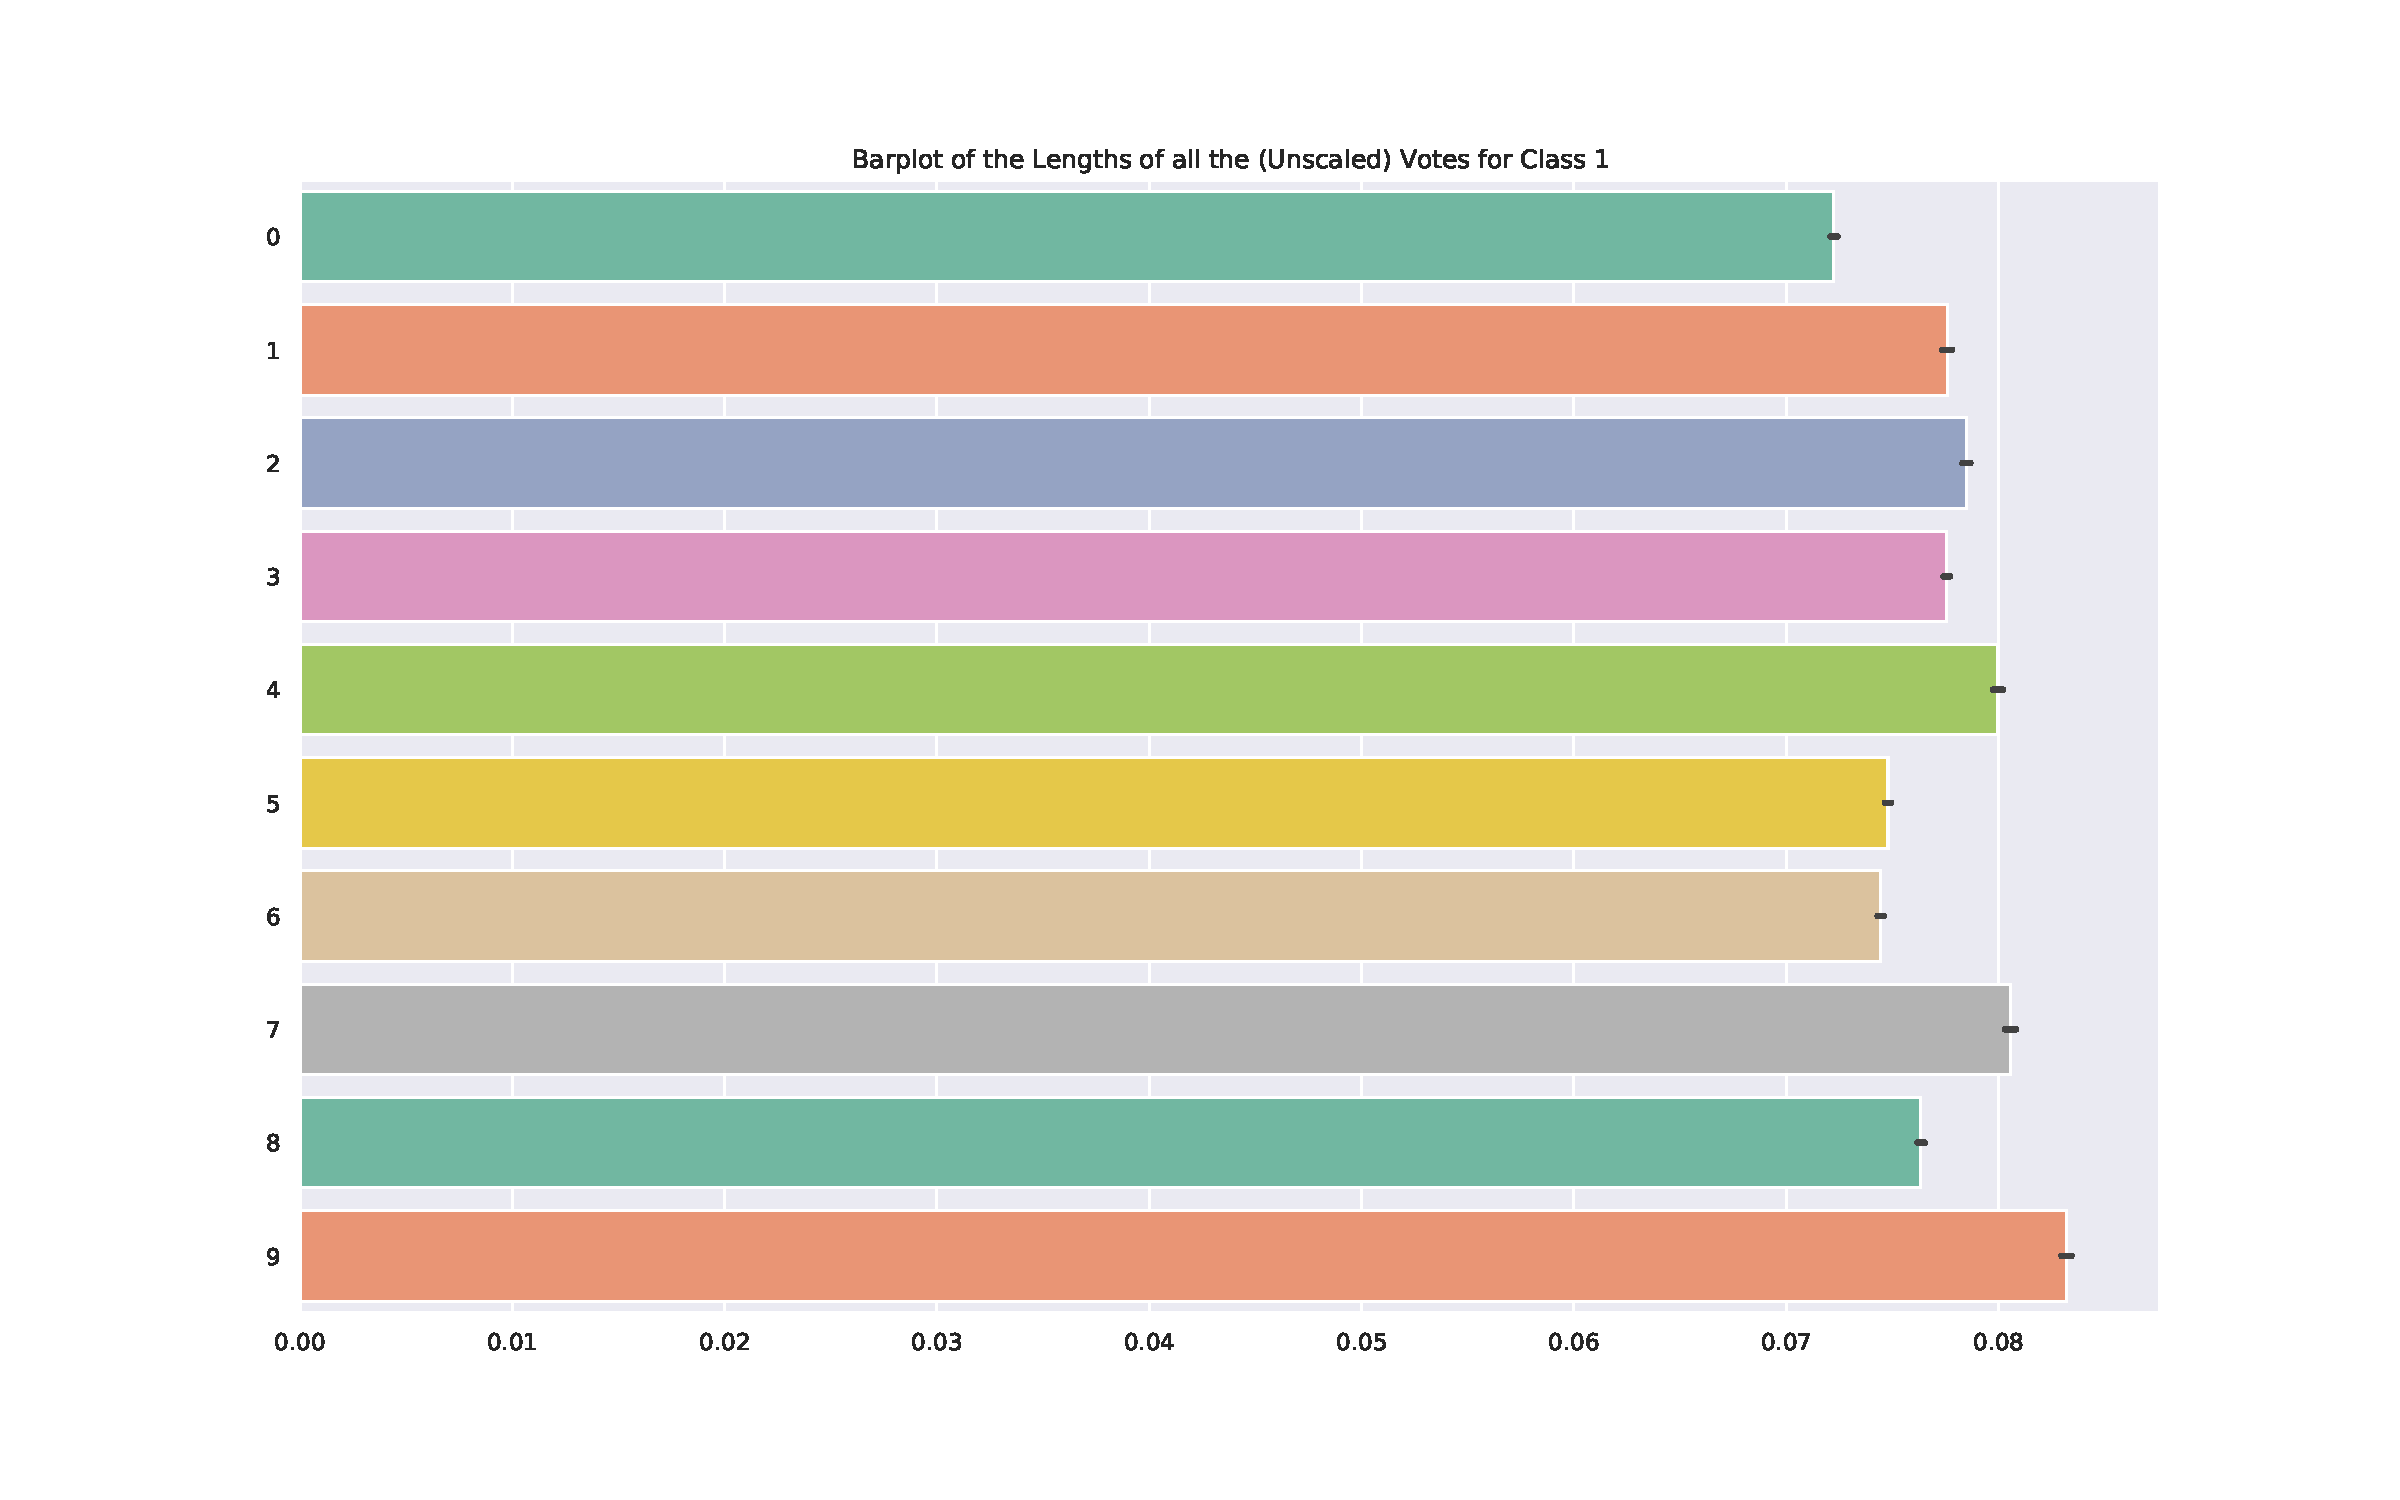
\includegraphics[ width=0.9\textwidth]{images/chapter experiments/method 1/image 12/barplot_for_class_1_unscaled_True.pdf}
    \caption{Γραφική παράσταση του μέσου μήκους των ψήφων ανά κλάση (όταν η ετικέτα είναι το ψηφίο 1).}
    \label{fig:exp_method_1_special_vote_dist_1}
  \end{figure}

\begin{figure}[h]

    \centering
    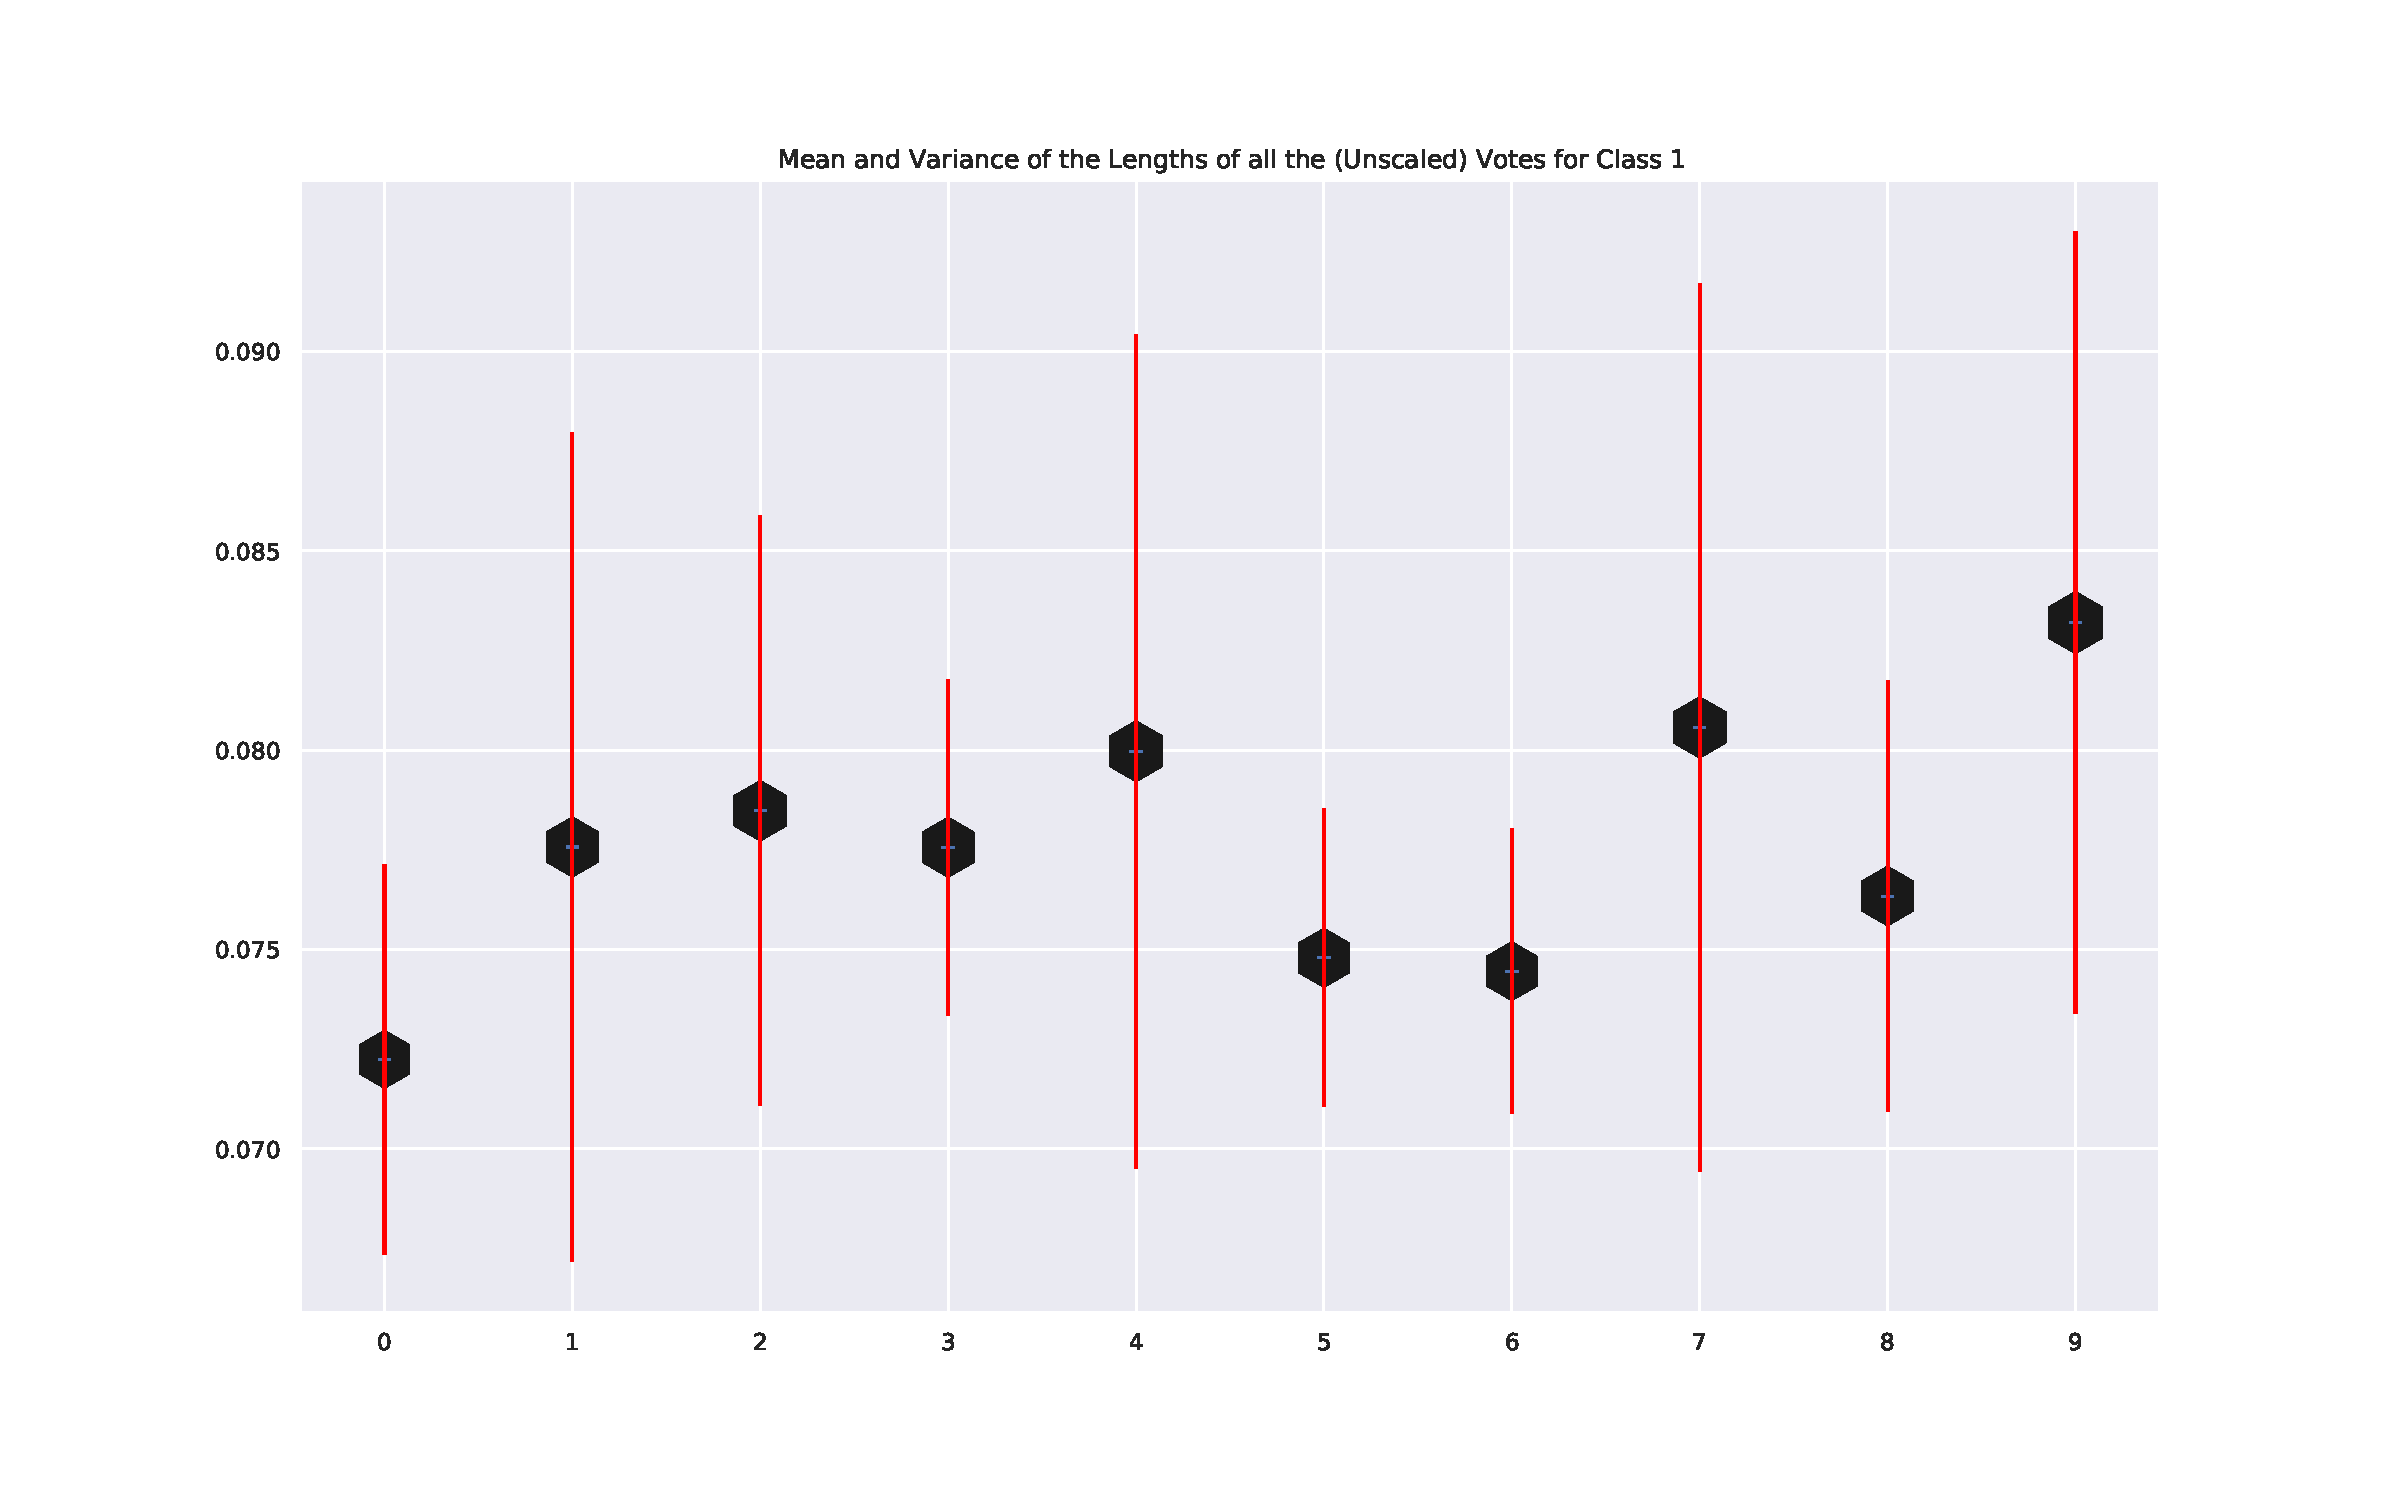
\includegraphics[width=0.9\textwidth]{images/chapter experiments/method 1/image 12/mean_var_for_class_1_unscaled_True.pdf}
    \caption{Γραφική παράσταση του μέσου μήκους των ψήφων ανά κλάση (όταν η ετικέτα είναι το ψηφίο 1). Στο διάγραμμα εμφανίζεται και η διασπορά με κόκκινες, κάθετες γραμμές.}
    \label{fig:exp_method_1_special_vote_dist_2}
    
  \end{figure}

Οπως φαίνεται από τις εικόνες \ref{fig:exp_method_1_special_vote_dist_1} και \ref{fig:exp_method_1_special_vote_dist_2} το μέτρο των αρχικών ψήφων (προτού κλιμακωθούν από τα βάρη δρομολόγησης) δεν φαίνεται να συσχετίζεται με κανέναν τρόπο με την κλάση πρόβλεψης. Να σημειώσουμε ότι τα εξής αποτελέσματα δεν αφορούν ένα μεμονωμένο παράδειγμα αλλά υπολογίζονται από τις ψήφους που προκύπτουν από (σχεδόν) όλα τα παραδείγματα της επιλεγμένης κλάσης στο σύνολο δεδομενων ελέγχου. Για αυτό άλλωστε και η διασπορά είναι τόσο μεγάλη.

\subsection{Κατανομή των Βαρών Δρομολόγησης}
% Ιστόγραμμα καθώς αυξάνονται οι επαναλήψεις.
Φαίνεται ότι τον καθοριστικό ρόλο της επίδοσης τον έχουν τα βάρη δρομολόγησης. Μάλιστα, από τα μέχρι τώρα πειράματα έχει φανεί πως η επιλογή της κλάσης στην οποία αντιστοιχεί η μέγιστη τιμή βάρους δρομολόγησης μπορεί να έχει καλύτερη επίδοση από τον κλασικό αλγόριθμο δρομολόγησης. Θέλωντας να εμβαθύνουμε στην κατανομή των βαρών δρομολόγησης μετά από τρείς επαναλήψεις, δημιουργούμε τρείς γραφικές παραστάσεις όπου έχουμε συγκεντρώσει τα βάρη δρομολόγησης από πάρα πολλά παραδείγματα του συνόλου ελέγχου που απεικονίζουν ένα συγκεκριμένο ψηφίο. Τα βάρη αυτά τα χωρίζουμε ανάλογα με το σε ποιά κάψουλα \en{DigitCap} απευθύνονται.\par
% image 13
\begin{figure}[h]
    \centering
    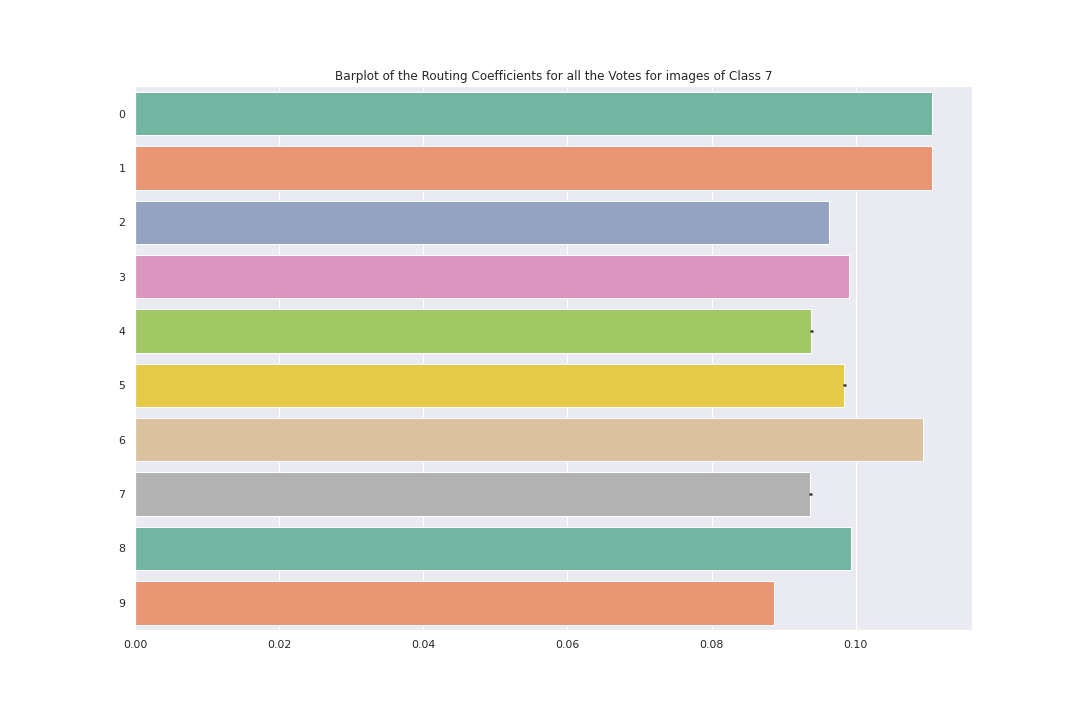
\includegraphics[width=0.9\textwidth]{images/chapter experiments/method 1/image 13/barplot_for_class_7.png}
    \caption{Γραφική παράσταση της μέσης τιμής των βαρών δρομολόγησης ανά κλάση.}
    \label{fig:exp_method_1_special_weight_dist_1}
  \end{figure}

\begin{figure}[h]
    \centering
    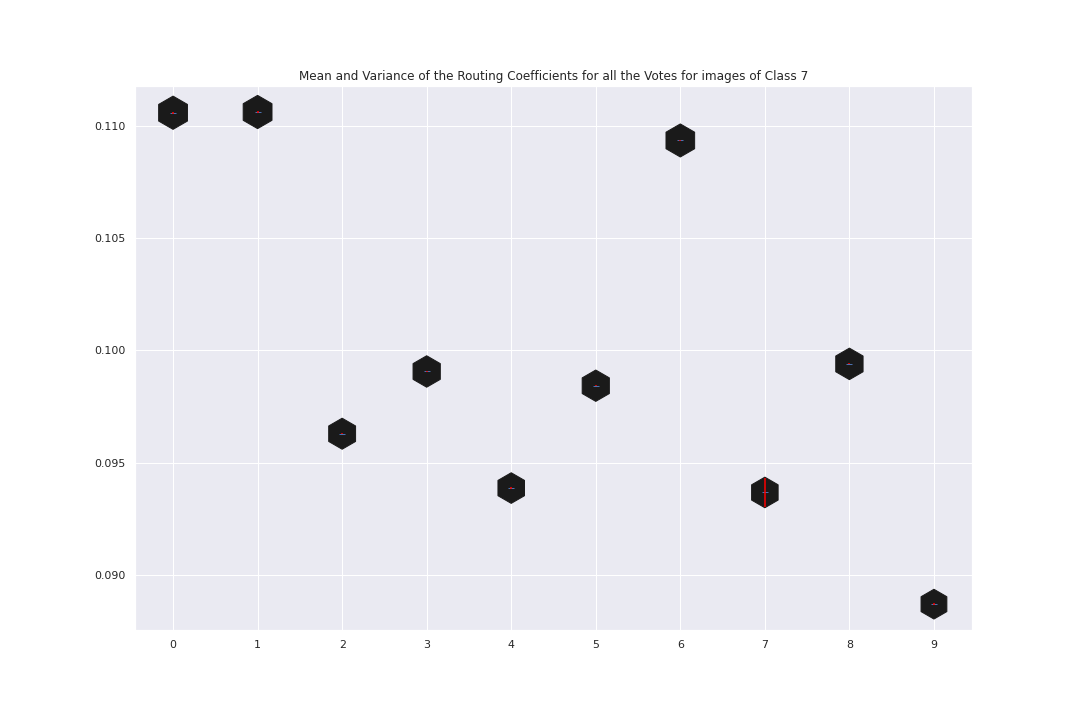
\includegraphics[width=0.9\textwidth]{images/chapter experiments/method 1/image 13/mean_var_for_class_7.png}
    \caption{Γραφική παράσταση της μέσης τιμής των βαρών δρομολόγησης ανά κλάση. Στο διάγραμμα εμφανίζεται και η διασπορά με κόκκινες, κάθετες γραμμές.}
    \label{fig:exp_method_1_special_weight_dist_2}
  \end{figure}

Από τα σχήματα \ref{fig:exp_method_1_special_weight_dist_1} και \ref{fig:exp_method_1_special_weight_dist_2} φαίνεται ότι η διασπορά είναι μεγαλύτερη για τα βάρη που αντιστοιχούν στις σωστές κάψουλες. Δεν μπορούμε όμως να διακρίνουμε την σωστή κλάση κοιτώντας τις μέσες τιμές. Αν όμως λάβουμε την μέγιστη τιμή των βαρών δρομολόγησης για την κάθε κάψουλα του τελευταίου επιπέδου, διαπιστώνουμε ότι πάντα η σωστή κλάση έχει βάρη δρομολόγησης με την μεγαλύτερη τιμή (βλέπε σχήμα \ref{fig:exp_method_1_special_weight_dist_3}).
\begin{figure}[h]
    \centering
    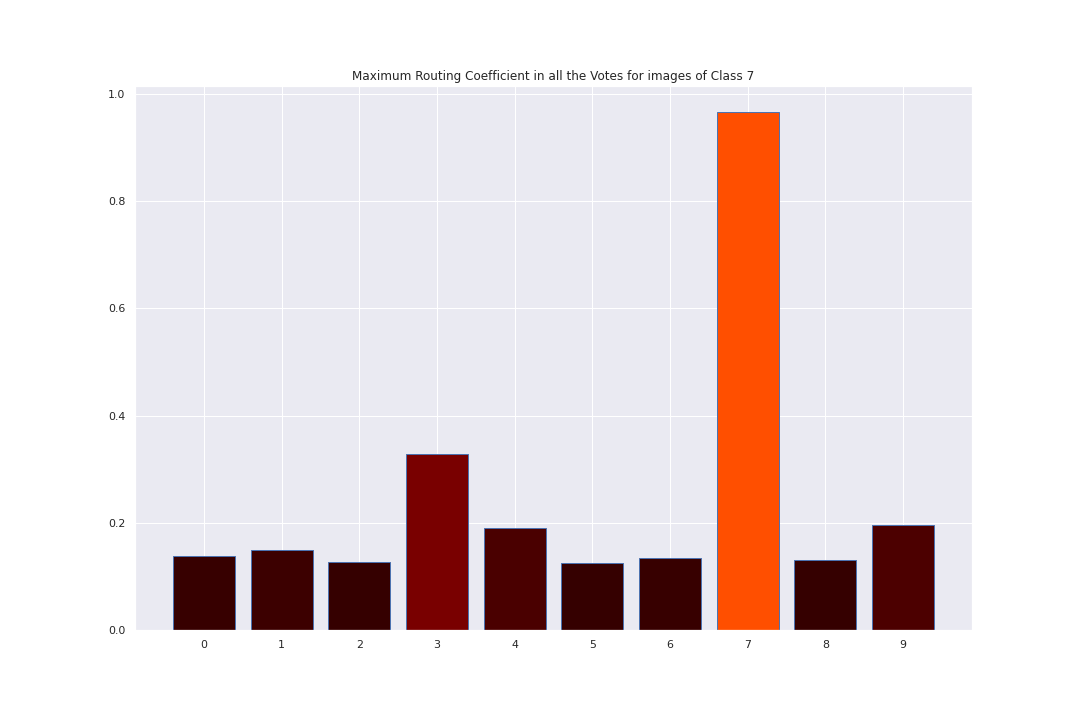
\includegraphics[width=0.9\textwidth]{images/chapter experiments/method 1/image 13/Max_for_class_7.png}
    \caption{Γραφική παράσταση της τιμής του μεγίστου βάρους δρομολόγησης ανά κλάση (για εικόνες εισόδου που απεικονίζουν το νούμερο 7).}
    \label{fig:exp_method_1_special_weight_dist_3}
  \end{figure}

\subsection{Ιστογράμματα των Σταθμισμένων Ψήφων ανα Αριθμό Επαναλήψεων}

Το τελευταίο πείραμα που πραγματοποιείται εξετάζει την κατανομή των μηκών των σταθμισμένων (από το αντίστοιχο βάρος δρομολόγησης) ψήφων, καθώς αυξάνονται οι επαναλήψεις του αλγορίθμου δυναμικής δρομολόγησης. Χρησιμοποιώντας τον συμβολισμό που εισαγάγαμε στο προηγούμενο κεφάλαιο, υπολογίζουμε τα ιστογράμματα των διανυσμάτων $V^L_{ij} \ast R^L_{ij}$ ομαδοποιημένων κατά κλάση $j$. Έτσι προκύπτουν τα σχήματα \ref{fig:exp_method_1_special_hist_r_3} , \ref{fig:exp_method_1_special_hist_r_2} και \ref{fig:exp_method_1_special_hist_r_1} μετά από 3, 2 και 1 επαναναλήψεις αντίστοιχα. Προφανώς, στην πρώτη επανάληψη τα μήκη εξαρτώνται από τους πίνακες μετασχηματισμού αφού τα βάρη δρομολόγησης είναι όλα ίσα. Σε επόμενες επαναλήψεις όμως, τα βάρη δρομολόγησης επηρεάζουν το μήκος των ψήφων με το να αποσιωπούν τις ψήφους σε κλάσεις με μικρή συμφωνία (που δεν αντιστοιχούν στην σωστή κλάση πρόβλεψης) και με το να ενισχύουν ορισμένες ψήφους που δρομολογούνται στην σωστή κλάση. Σημειώνουμε ότι τα ιστογράμματα βρίσκονται σε λογαριθμική κλίμακα και για την παραγωγή τους λήφθηκαν υπόψη τα περισσότερα δείγματα του συνόλου ελέγχου που αφορούν την συγκεκριμένη κλάση στόχο (ο λόγος που δεν λήφθηκαν όλα υπόψη είναι καθαρά υπολογιστικός).
% image 14
\begin{figure}[h]
    \centering
    
\includegraphics[trim={14cm 0 13cm 0},clip, width=0.99\textwidth]{images/chapter experiments/method 1/image 14/hists_for_class_1_r_3.png}
    \caption{Ιστογράμματα του μήκους των ψήφων σταθμισμένων από τα αντίστοιχά τους βάρη δρομολόγησης μετά την τρίτη επανάληψη του δυναμικού αλγορίθμου δρομολόγησης.}
    \label{fig:exp_method_1_special_hist_r_3}
  \end{figure}

  \begin{figure}[h]
    \centering
    
\includegraphics[trim={14cm 0 13cm 0},clip, width=0.99\textwidth]{images/chapter experiments/method 1/image 14/hists_for_class_1_r_2.png}
    \caption{Ιστογράμματα του μήκους των ψήφων σταθμισμένων από τα αντίστοιχά τους βάρη δρομολόγησης μετά την δεύτερη επανάληψη του δυναμικού αλγορίθμου δρομολόγησης.}
    \label{fig:exp_method_1_special_hist_r_2}
  \end{figure}

  \begin{figure}[h]
    \centering
    
\includegraphics[trim={14cm 0 13cm 0},clip, width=0.99\textwidth]{images/chapter experiments/method 1/image 14/hists_for_class_1_r_1.png}
    \caption{Ιστογράμματα του μήκους των ψήφων σταθμισμένων από τα αντίστοιχά τους βάρη δρομολόγησης μετά την πρώτη επανάληψη του δυναμικού αλγορίθμου δρομολόγησης.}
    \label{fig:exp_method_1_special_hist_r_1}
  \end{figure}


\section{Πειραματική Μελέτη Μεθόδου 2}
Σε αυτή την ενότητα παρουσιάζουμε ορισμένα από τα πειράματα που πραγματοποιήθηκαν στον αλγόριθμο δρομολόγησης βασισμένο στον \en{EM}. Συγκεκριμένα, πειραματιστήκαμε με δύο υλοποιήσεις στην γλώσσα \en{tensorflow}. Η πρώτη υλοποίηση είναι αυτή της \en{IBM} και περιγράφεται αναλυτικά στο έργο \cite{gritzman2019avoiding}. Η δεύτερη αποτελεί την αυθεντική υλοποίηση του έργου \cite{hinton2018matrix} και εντοπίζεται σε αυτή την \href{https://git.informatik.uni-hamburg.de/0moin/google-research/-/commits/master/capsule_em}{ιστοσελίδα}. Αν και η δεύτερη, πολύπλοκη υλοποίηση από την ομάδα της \en{Google Brain} επέτρεπε την εκπαίδευση και δοκιμή μόνο στο σύνολο δεδομένων \en{smallNORB} με τις κατάλληλες επεκτάσεις επιδιώξαμε να εκπαιδεύσουμε το δίκτυο και στο σύνολο δεδομένων \en{MNIST}. Προφανώς, όλη η προεπεξεργασία των συνόλων δεδομένων είναι ίδια με αυτή του έργου \cite{hinton2018matrix}. Επίσης, κατασκευάσαμε εκ νέου ένα αρχείο \en{Docker} για την κατασκευή εικονικού περιβάλλοντος με όλες τις κατάλληλες εκδόσεις λογισμικού. Να σημειώσουμε ότι καμία από τις δύο υλοποιήσεις δεν ήταν σε πλήρη μορφή καθώς δεν προορίζονταν για εκπαίδευση. Χρειάστηκε να γίνουν αρκετές αλλαγές προκειμένου να προσαρμοστούν στις δικές μας απαιτήσεις.\par

Προτού παρουσιάσουμε τα πειράματα που έγιναν στην μέθοδο δύο, να αναφέρουμε ότι πειραματιστήκαμε για λίγες εποχές και με ορισμένες άλλες επιλογές που παρέχουν οι υλοποιήσεις. Παρόλα αυτά, τα συμπεράσματα ήταν ασαφή για τις λίγες εποχές εκπαίδευσης. Μερικές από τις παραμετροποιήσεις που μπορούν να δοκιμαστούν είναι ο αριθμός των καψουλών του επιπέδου \en{Primary Capsules}, το μέγεθος των πυρήνων των πρώτων επιπέδων και ο αριθμός των φίλτρων τους, την προσθήκη επιπλέον συνελικτικών επιπέδων με ή χωρίς κάψουλες, την χρήση του μηχανισμού \en{dropout}, την χρήση ενός συνόλου ίδιων μοντέλων εκπαιδευμένων στο ίδιο σύνολο για την δοκιμή στο σύνολο ελέγχου (\en{ensemble}) κτλ.\par

Παρακάτω θα παρουσιάσουμε τα πειράματα που έγιναν σε περιορισμένο αριθμό επαναλήψεων για δύο διαφορετκούς αριθμούς επαναλήψεων (2 και 3) του αλγορίθμου δρομολόγησης. Αν και το μοντέλο δεν έχει πολλές εκπαιδευόμενες παραμέτρους ($310k$) η υπολογιστική του πολυπλοκότητα είναι περίπου πέντε φορές μεγαλύτερη (\en{0.401 operations per batch versus 0.086 operations per batch}). Αυτό δεν μας επέτρεψε να διενεργήσουμε εκτενή πειράματα καθώς και επίσης να χρησιμοποιήσουμε μεγάλο μέγεθος δέσμης.

\subsection{\en{SmallNORB}}
Για να διερευνήσουμε την επίδραση του αριθμού των επαναλήψεων στην ακρίβεια του αλγορίθμου στο σύνολο \en{SmallNORB}, εκπαιδεύσαμε το μοντέλο με τον αλγόριθμο δρομολόγησης βασισμένο στον \en{EM} (αλγόριθμος \ref{alg:em_routing}) για 15000 βήματα με σύνολο δέσμης ίσο με 8 (το μέγιστο δυνατό) το οποίο ισοδυναμεί με 5 επόχές. Τα αποτελέσματα που λάβαμε παρουσιάζονται στον πίνακα \ref{tab:method_2_smallNORB_rout_iter}.
\begin{table}[h]
    \begin{center}
        \en{
        \begin{tabular}{c c c c}
            \toprule
            Dataset & Routing Iterations & Test Error (\%) \\ 
            \midrule
            SmallNORB & 2 & \textbf{14.04} \\
            SmallNORB & 3 & 63.49 \\
            \bottomrule
        \end{tabular}
        }
    \end{center}
    \caption[]{\label{tab:method_2_smallNORB_rout_iter}Πίνακας στον οποίο φαίνεται η επίδραση του αριθμού των επαναλήψεων στην ακρίβεια όπως μετράται από το σύνολο ελέγχου \en{SmallNORB}, όταν χρησιμοποιούνται πολύ λίγες εποχές για την εκπαίδευση του μοντέλου.} 
\end{table}

Όπως προδίδουν τα αποτελέσματα, ειδικά όταν χρησιμοποιείται μικρό σύνολο δέσμης, ο αλγόριθμος είναι πιθανό να βρεθεί σε αστάθεια. Φυσικά, γνωστά προβλήματα του αλγορίθμου \en{EM} όπως το \en{variance collapse} δεν διευκολύνουν την διαδικασία εκπαίδευσης με αποτέλεσμα αυτή να γίνεται όλο και πιο ασταθής καθώς αυξάνονται οι επαναλήψεις. Στις εικόνες \ref{fig:method2_smallnorb_exp_left} και \ref{fig:method2_smallnorb_exp_right} παρουσιάζονται το συνολικό σφάλμα και η ακρίβεια (μέγιστη ακρίβεια είναι 1) για τις δύο περιπτώσεις του πίνακα \ref{tab:method_2_smallNORB_rout_iter} (με κόκκινο απεικονίζεται η εκπαίδευση για 2 επαναλήψεις ενώ με μπλέ για 3). Παρατηρούμε ότι στην περίπτωση των 3 επαναλήψεων ο αλγόριθμος μπαίνει σε κατάσταση αστάθειας και δεν ανακάμπτει μέχρι το τέλος της εκπαίδευσης.
% image 1
% \begin{figure}
%     \centering
%     \begin{minipage}{.5\textwidth}
%       \centering
%       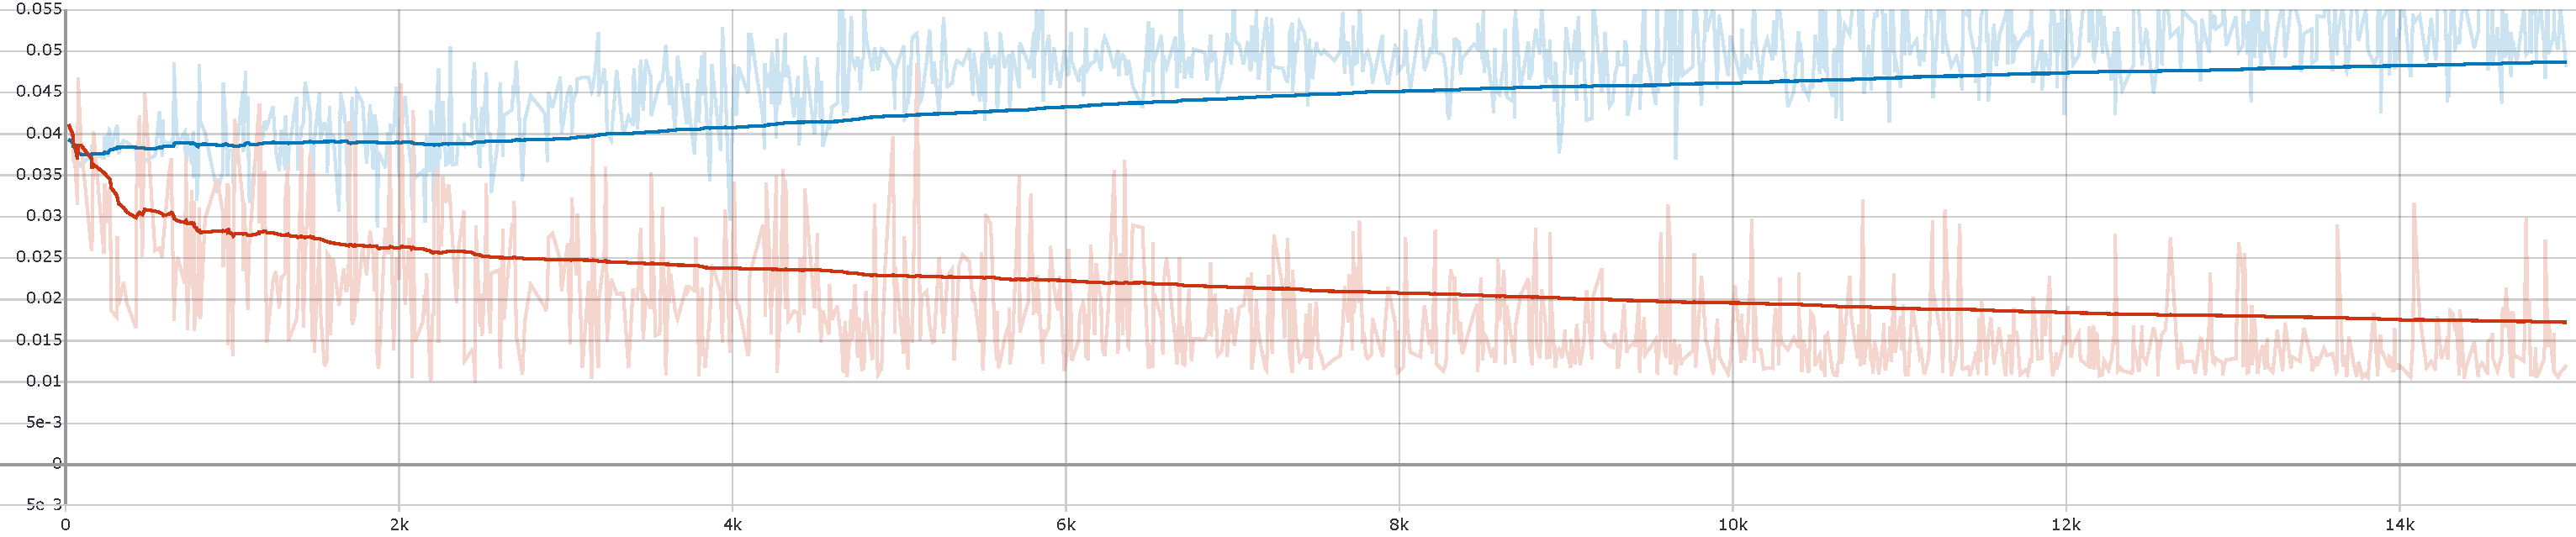
\includegraphics[width=.4\linewidth]{images/chapter experiments/method 2/tower_0_total_loss_1.pdf}
%       \captionof{figure}{Συνολικό σφάλμα μετρούμενο κατά την εκπαίδευση για τον αλγόριθμο \en{EM} της 2\textsuperscript{ης} μεθόδου με αριθμό επαναλήψεων 2 (κόκκινο) ή 3 (μπλέ).}
%       \label{fig:method2_smallnorb_exp_left}
%     \end{minipage}%
%     \begin{minipage}{.5\textwidth}
%       \centering
%       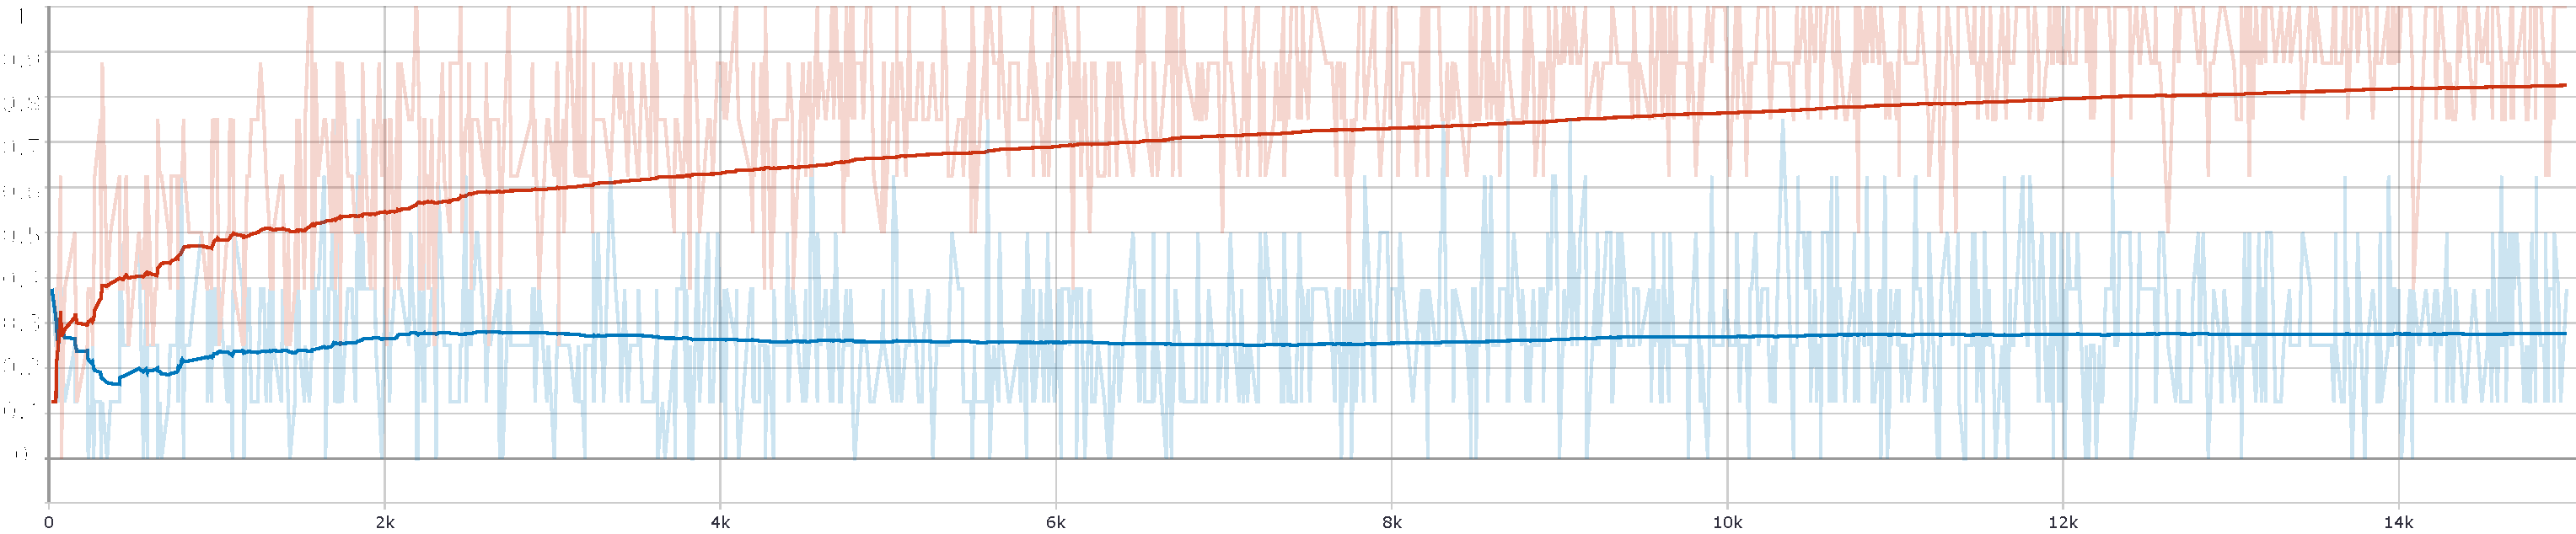
\includegraphics[width=.4\linewidth]{images/chapter experiments/method 2/tower_0_accuracy_1.pdf}
%       \captionof{figure}{Ακρίβεια μετρούμενη κατά την εκπαίδευση για τον αλγόριθμο \en{EM} της 2\textsuperscript{ης} μεθόδου με αριθμό επαναλήψεων 2 (κόκκινο) ή 3 (μπλέ).}
%       \label{fig:method2_smallnorb_exp_right}
%     \end{minipage}
%     \end{figure}

    \begin{figure}[h]
        \centering
        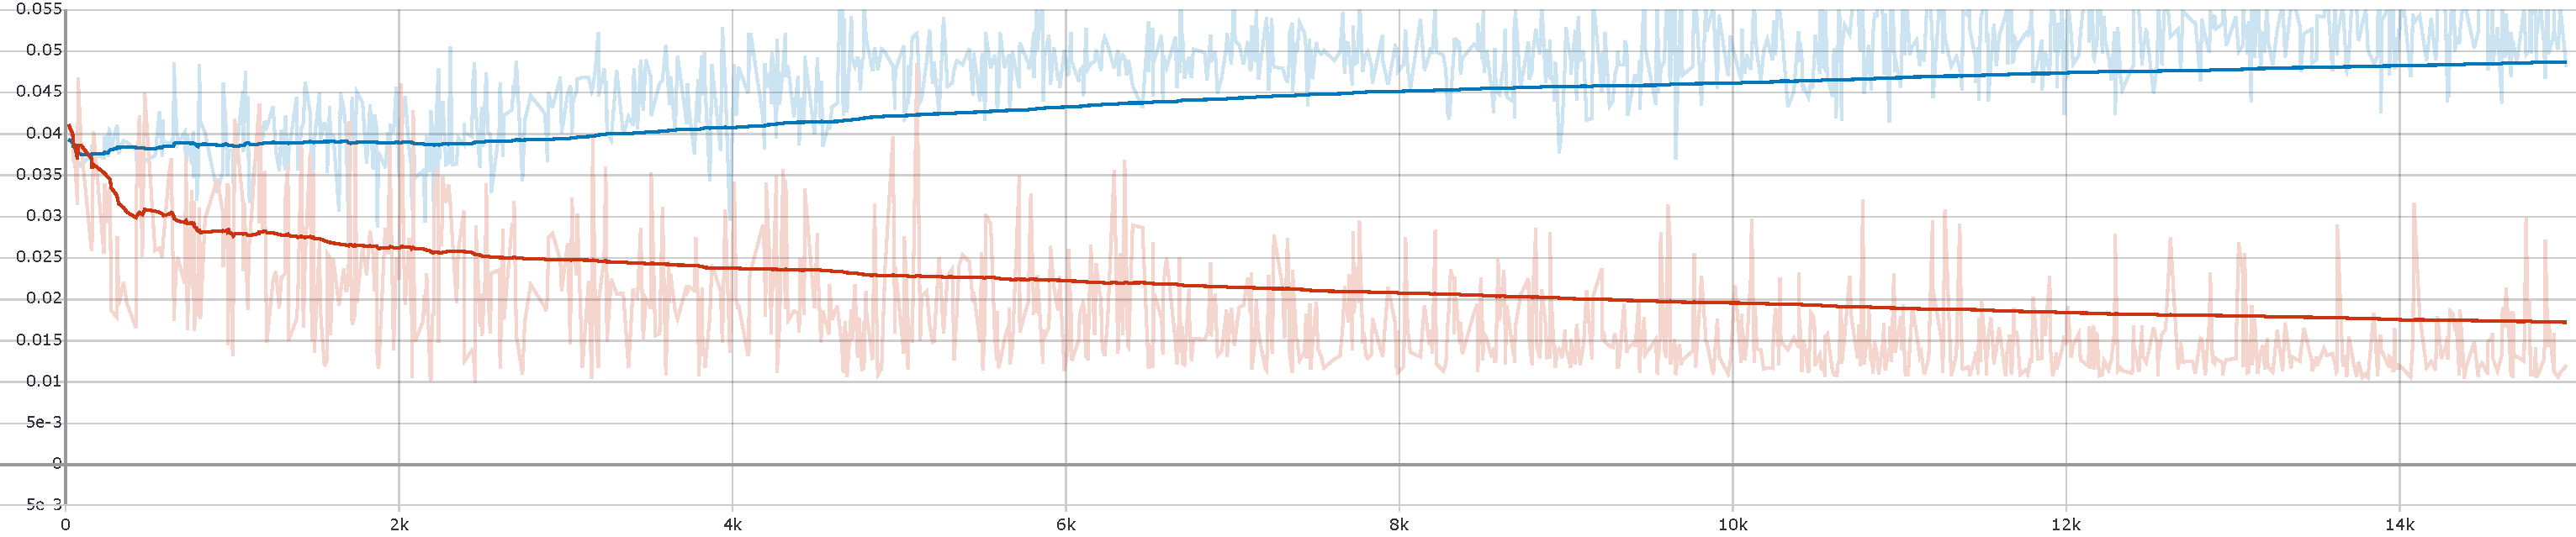
\includegraphics[ width=0.99\textwidth]{images/chapter experiments/method 2/tower_0_total_loss_1.pdf}
        \caption{Συνολικό σφάλμα μετρούμενο κατά την εκπαίδευση για τον αλγόριθμο \en{EM} της 2\textsuperscript{ης} μεθόδου με αριθμό επαναλήψεων 2 (κόκκινο) ή 3 (μπλέ).}
        \label{fig:method2_smallnorb_exp_left}
      \end{figure}

      \begin{figure}[h]
        \centering
        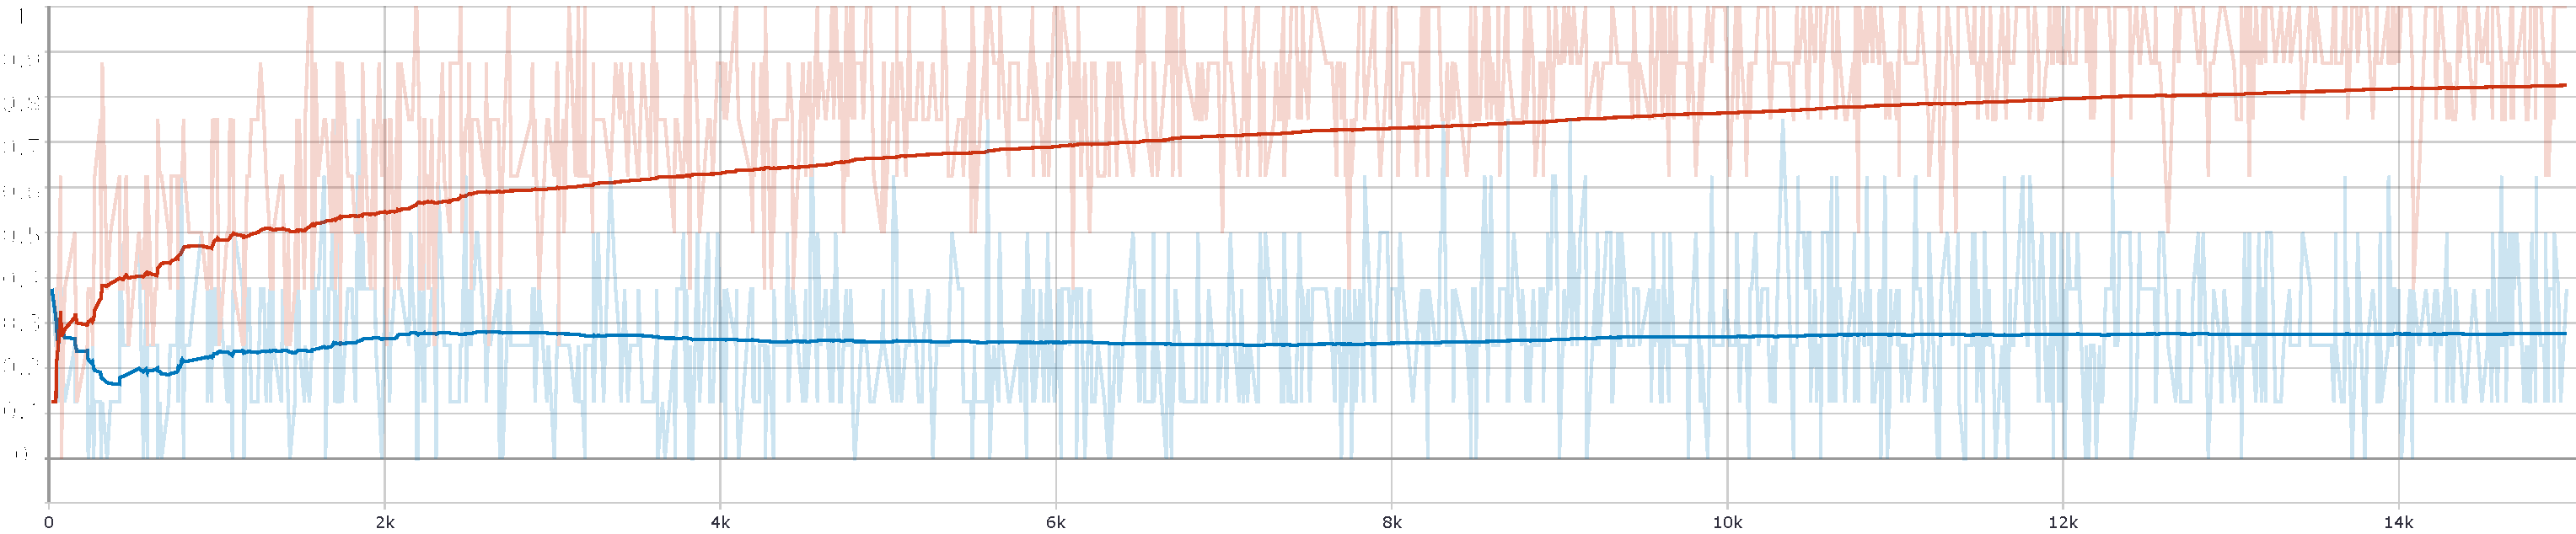
\includegraphics[ width=0.99\textwidth]{images/chapter experiments/method 2/tower_0_accuracy_1.pdf}
        \caption{Ακρίβεια μετρούμενη κατά την εκπαίδευση για τον αλγόριθμο \en{EM} της 2\textsuperscript{ης} μεθόδου με αριθμό επαναλήψεων 2 (κόκκινο) ή 3 (μπλέ).}
        \label{fig:method2_smallnorb_exp_right}
      \end{figure}

\subsection{\en{MNIST}}

Συνεχίζουμε με τη διερεύνηση της επιρροής του αριθμού των επαναλήψεων στην ακρίβεια του αλγορίθμου στο σύνολο δεδομένων \en{MNIST}. Και πάλι εκπαιδεύσαμε το μοντέλο με τον αλγόριθμο δρομολόγησης βασισμένο στον \en{EM} (αλγόριθμος \ref{alg:em_routing}) για 15000 βήματα με σύνολο δέσμης ίσο με 8 το οποίο ισοδυναμεί σε αυτή τη περίπτωση με μόλις 4 εποχές. Τα αποτελέσματα που λάβαμε εμφάνιζαν (λόγω και του μικρού συνόλου δέσμης) μεγάλο βαθμό αστάθειας και συνεπώς δεν ήταν αξιοσημείωτα.

\subsection{Δοκιμή στο \en{SmallNORB} με \en{Pretrained Model}}
Τέλος, δοκιμάσαμε την επίδοση του αλγορίθμου στο σύνολο δεδομένων \en{SmallNORB} με την χρήση ενός προ\textendash εκπαιδευμένου μοντέλου (από το διαδίκτυο) με βάρη που σχηματίστικαν κατά την διάρκεια πολύ περισσότερων εποχών. Τα αποτελέσματα, παρουσιάζονται στον πίνακα \ref{tab:method_2_last_matrix} και είναι ίδια με αυτά που παρουσιάζονται στο σχετικό έργο \cite{hinton2018matrix} επιβεβαιώνοντας έτσι ότι οι αλλαγές που προκαλέσαμε στον κώδικα δεν επιβάρυναν την επίδοση. Στον σχετικό πίνακα συγκρίνονται οι δύο χρησιμοποιούμενες υλοποιήσεις του αλγορίθμου. Όπως φαίνεται, η υλοποίηση που χρησιμοποιούμε (μαζί με τις αλλαγές μας που δεν επηρεάζουν τον βασικό αλγόριθμο) εμφανίζει την καλύτερη επίδοση (μετρημένη με την χρήση του \en{pre\textendash trained} μοντέλου).\par

\begin{table}[h]
    \begin{center}
        \en{
        \begin{tabular}{c c c c}
            \toprule
            Implementation & Framework & r & Test Error (\%) \\ 
            \midrule
            Hinton et al.\cite{hinton2018matrix} & tensorflow & 3 & 1.8 (1.4*) \\
            Hinton et al. + Our modifications & tensorflow & 3 & \textbf{1.8 (1.3*)} \\
            Matrix Capsules IBM \cite{gritzman2019avoiding}& tensorflow & 2 & 4.6 \\
            Matrix Capsules IBM \cite{gritzman2019avoiding}& tensorflow & 3 & 6.3 \\
            \bottomrule
        \end{tabular}
        }
    \end{center}
    \caption[]{\label{tab:method_2_last_matrix}Πίνακας στον οποίο συγκρίνονται οι επιδόσεις των δύο χρησιμοποιούμενων υλοποιήσεων της μεθόδου 2 (αλγόριθμος \ref{alg:em_routing}) στο σύνολο δεδομένων \en{SmallNORB}. Για την δεύτερη υλοποίηση, δεν υπήρχε διαθέσιμο κάποιο προ\textendash εκπαιδευμένο μοντέλο για να δοκιμάσουμε τα επικαλούμενα αποτελέσματα. Σημειώνουμε ότι το αστεράκι σημαίνει ότι η πρόβλεψη προκύπτει από την μέση τιμή των προβλέψεων τυχαίων παραθύρων (\en{random crops}) της ίδιας εικόνας. Η βελτιωμένη επίδοση μετά τις δικές μας αλλαγές δεν οφείλεται σε αυτές αλλά στον καλύτερο, \en{pre-trained} μοντέλο που χρησιμοποιούμε.} 
\end{table}


\section{Πειραματική Μελέτη Μεθόδου 3}
\label{sec:method_3_experiments}
Στην ενότητα αυτή θα πειραματιστούμε με τους γρήγορους αλγορίθμους δρομολόγησης με μηχανισμό αυτοπροσοχής που παρουσιάσαμε στην ενότητα \ref{sec:method_3}. Υπενθυμίζεται ότι στην ενότητα αυτή παρουσιάστηκαν τέσσερεις αλγόριθμοι καθώς και οι παραλλαγές τριών εξ' αυτών για την περίπτωση που χρησιμοποιείται μηχανισμός πολυκέφαλης προσοχής (\en{multiheadd attention}). Οι τέσσερεις αλγόριθμοι και οι τρείς πολυκέφαλες παραλλαγές τους που παρουσιάστηκαν στην σχετική μέθοδο είναι με την σειρά οι εξής: 
\begin{itemize}
    \item \textquote{Απλοικός Αλγόριθμος Δρομολόγησης με Αυτο\textendash Προσοχή} (αλγόριθμος \ref{alg:method3_stupid_routing})
    \item \textquote{Αλγόριθμος \en{RoMAV}} (αλγόριθμος \ref{alg:method3_sum_routing})
    \item \textquote{Αλγόριθμος \en{RoWSS}} (αλγόριθμος \ref{alg:method3_max_routing})
    \item \textquote{Αλγόριθμος \en{RoWLS}} (αλγόριθμος \ref{alg:method3_max_len_routing})
    \item \textquote{Αλγόριθμος \en{Multihead RoMAV}} (αλγόριθμος \ref{alg:method3_sum_multihead_routing})
    \item \textquote{Αλγόριθμος \en{Multihead RoWSS}} (αλγόριθμος \ref{alg:method3_max_multihead_routing})
    \item \textquote{Αλγόριθμος \en{Multihead RoWLS}} (αλγόριθμος \ref{alg:method3_max_len_multihead_routing})
\end{itemize}

Ο πρώτος στην λίστα, απλοικός αλγόριθμος μιας και αποτελεί έργο των \en{Mazzia V. et al.}\cite{mazzia2021efficient} στο οποίο παρουσιάζονται εκτενή πειράματά του, δεν συμμετέχει στο πειραματικό μέρος αυτής της ενότητας. Αντίθετα, οι άλλοι (δικοί μας) αλγόριθμοι δοκιμάζονται με πειράματα των οποίων στόχος είναι η πιστοποίηση μιας γρήγορης, κλιμακώσιμης αρχιτεκτονικής νευρωνικών δικτύων με κάψουλες. Για τα πειράμτα αυτά, χρησιμοποιούνται όλα τα απαραίτητα σύνολα δεδομένων που σε ένα βαθμό ελέγχουν την τήρηση των ιδιοτήτων των νευρωνικών δικτύων με κάψουλες. Τα σύνολα δεδομενων είναι τα \en{MNIST}, \en{CIFAR10}, \en{SmallNORB} και \en{multiMNIST} με τα τελευταία δύο να εξετάζουν την ικανότητα του νευρωνικού δικτύου από κάψουλες να γενικεύει σε νέες οπτικές γωνίες (\en{SmallNORB}) και να χειρίζεται αποδοτικά μερική επικάλυψη των εικόνων (\en{multiMNIST}) αντίστοιχα.\par

Εστιάζοντας ακόμα περισσότερο στα σύνολα δεδομένων που χρησιμοποιούνται στα πειράματα της τρίτης μεθόδου, η προεπεξεργασία τους διαφέρει από αυτή που παρουσιάσαμε στα περιάματα της μεθόδου 1. Αναλυτικότερα, για κάθε σύνολο δεδομένων κάνουμε τα εξής:
\begin{description}
    \item[\en{MNIST}] Ακολουθούμε την προεπεξεργασία που προτείνεται στο έργο \cite{byerly2020branching}. Μέγεθος εισόδου: [$28 \times 28 \times 1$]
    \item[\en{FashionMNIST}] Ίδια προεπεξεργασία με το σύνολο δεδομένων \en{MNIST}. Μέγεθος εισόδου: [$28 \times 28 \times 1$]
    \item[\en{CIFAR10}] Διαιρούμε όλα τα στοιχεία με την τιμή $255$ προκειμένου να ανήκουν στο σύνολο $[0,1]$. Έπειτα λαμβάνουμε κεντρικά παράθυρα $28 \times 28$ των εικόνων αρχικού μεγέθους $32 \times 32$ Μέγεθος εισόδου [$28 \times 28 \times 3$].
    \item[\en{smallNORB}] Ακολουθούμε Κλιμάκωση σε μέγεθος $64 \times 64$ (από το αρχικό μέγεθος που είναι $96 \times 96$), κάνουμε περικοπή σε ένα παράθυρο μεγέθους $48 \times 48$ και τέλος, προσθέτουμε τυχαία φωτεινότητα και αντίθεση στο σύνολο εκπαίδευσης (παρόμοια με το έργο \cite{hinton2018matrix}). Επειδή το σύνολο αποτελείται από στερεοπτικές εικόνες, τις στοιβάζουμε δημιουργώντας μια εικόνα με δύο κανάλια. Μέγεθος εισόδου μετά από προεπεξεργασία: [$48 \times 48 \times 2$].
    \item[\en{MultiMNIST}] Αρχικά, γεμίζουμε το περιθώριο της κάθε εικόνας του συνόλου δεδομένων \en{MNIST} περιμετρικά με μηδενικά προκειμένου το νέο μέγεθος της εικόνας να είναι $36 \times 36$. Μια εικόνα \en{MultiMNIST} προκύπτει από την εναπόθεση των δύο εικόνων μεταξύ τους με μια πιθανή ολίσθηση μέχρι 4 εικονοστοιχεία στον $x-y$ άξονα. Κατά την εκπαίδευση, παράγουμε 2 \en{MultiMNIST} εικόνες για κάθε εικόνα στο αρχικό σύνολο δεδομένων \en{MNIST}. Το σύνολο ελέγχου είναι δεκαπλάσιο από το αντίστοιχο σύνολο του \en{MNIST} και προκύπτει από την παραγωγή, για κάθε (βασική) εικόνα του αρχικού συνόλου, 10 εικόνων που αποτελούν το συσσωμάτωμα της βασικής εικόνας με 10 τυχαίες (διαφορετικού ψηφίου). Μέγεθος εισόδου [$36 \times 36 \times 2$].
\end{description} 

Αναφορικά με τις λεπτομέρειες υλοποίησης, χρησιμοποιείται ο βελτιστοποιητής \en{nAdam} ενώ σε λίγες περιπτώσεις δοκιμάζεται ο βελτιστοποιητής \en{Adam} (όπου γίνεται η χρήση του θα αναγράφεται με ρητό τρόπο). Στις περιπτώσεις που χρησιμοποιείται ανακατασκευαστής, εκτός από το σφάλμα \en{Margin Loss} έχουμε και το σφάλμα που προκύπτει από την ανακατασκευή (\en{MSE loss}). Τα δύο σφάλματα αθροίζονται και διαμορφώνουν το συνολικό σφάλμα εκπαίδευσης, όπως στην περίπτωση της μεθόδου \ref{sec:method_1}. Η διαφορά έγκειται στο ότι το σφάλμα ανακατασκευής κλιμακώνεται προτού αθροιστεί με το σφάλμα \en{Margin loss} με τον παράγοντα 0.2. Επιπλέον, αξίζει να αναφέρουμε ότι σε ορισμένες περιπτώσεις δοκιμάζουμε εκθετικό πρόγραμμα μείωσης του ρυθμού μάθησης (\en{exponential decay}) τον οποίο και θέτουμε στην τιμή $0.001$.\par

Στις επόμενες υπο\textendash ενότητες παρουσιάζονται τα πειράματα που έγιναν με τους διαθέσιμους αλγορίθμους. Δυστυχώς, οι περιορισμένοι πόροι δεν μας επέτρεψαν να κάνουμε μια εξονυχιστική αναζήτηση στον χώρο των υπερπαραμέτρων για την κάθε μέθοδο ξεχωριστά και για το κάθε σύνολο δεδομένων. Άλλωστε, σκοπός μας σε αυτή τη μέθοδο είναι να παρακινήσουμε την έρευνα προς μια υποσχόμενη αρχιτεκτονική που αναπτύξαμε στην τρίτη μέθοδο καταδεικνύοντας αρκετά καλά αποτελέσματα που μπορούν να βελτιωθούν σημαντικά με περαιτέρω αναζήτηση των βέλτιστων υπερπαραμέτρων.\par

\subsection{Αναζήτηση στον Χώρο των Υπερπαραμέτρων}
Στην υποενότητα αυτή παρουσιάζουμε ορισμένα από τα πειράματα που έγιναν στο πλαίσιο αναζήτησης των βέλτιστων υπερπαραμέτρων για τους αλγορίθμους μας. Οι υπερπαράμετροι για τις οποίες αναζητήσαμε την βέλτιστη τιμή συμπεριλαμβάνουν την χρήση ή μη πολυκέφαλης προσοχής, τη χρήση ή μη ανακατασκευαστή (αλλά και το είδος του ανακατασκευαστή) αλλά και ειδικές - για τον κάθε αλγόριθμο - υπερπαραμέτρους όπως η κλιμάκωση των εκπροσώπων με το αντίστοιχο σκόρ ομοιότητας (\en{Similarity Score}) και η ομαλή μεγιστοποίηση ή όχι των \en{similarity scores}.\par

Το σύνολο στο οποίο γίνεται η αναζήτηση των υπερπαραμέτρων είναι το \en{SmallNORB}. Επιλέξαμε το συγκεκριμένο σύνολο καθώς τα περισσότερα νευρωνικά δίκτυα με κάψουλες εξετάζουν την επίδοσή τους σε αυτό γεγονός που επιτρέπει τη σύγκριση των επιδόσεών τους. Επίσης, είναι ένα πιό σύνθετο σύνολο δεδομένων από το \en{MNIST} γεγονός που διακρύνει άμεσα τις παραμετροποιήσεις που οδηγούν σε μοντέλα με μέτριες επιδόσεις.\par

Δυστυχώς, οι υπολογιστικοί πόροι που έχουμε στην διαθεσιμότητά μας δεν μας επιτρέπουν να πειραματιστούμε με την εναλλακτική αρχιτεκτονική των πρώτων επιπέδων (αυτή δηλαδή που ακολουθεί και το έργο \cite{hinton2018matrix} και όχι αυτή που παρουσιάσαμε στο σχήμα \ref{fig:method_1_architecture}). Αυτό συμβαίνει διότι η διαδικασία εξαγωγής καψουλών που ακολουθείται στο έργο \en{Dynamic Routing Between Capsules}\cite{sabour2017dynamic} παράγει πολύ μεγάλο αριθμό από \en{Primary Capsules} οι οποίες λόγω του αλγορίθμου δρομολόγησής μας, θα πρέπει να συγκριθούν μεταξύ τους (μέσω των παραγόμενων ψήφων τους). Συνεπώς, τα παρακάτω αποτελέσματα αφορούν την αρχιτεκτονική \en{DepthConv}. Σε κάθε περίπτωση, μια τέτοια υλοποίηση θα ξέφευγε από τους σκοπούς της μεθόδου για την ανάπτυξη μιας κλιμακώσιμης (\en{scalable}) και γρήγορης αρχιτεκτονικής νευρωνικών δικτύων με κάψουλες.\par

Σαν μια προσπάθεια ελάττωσης της υπερπροσαρμογής του δικτύου στα δεδομένα εκπαίδευσης, εφαρμόσαμε \en{Dropout} μετά τα πρώτα δύο συνελικτικά επίπεδα με παράμετρο $p_{value} 0.2$, όπως είθισται για την περίπτωση των συνελικτικών δικτύων.\par

Εκτός από τα πειράματα στις παραμέτρους που εμφανίζονται στους πίνακες που ακολουθούν, έγιναν επιπλέον μελέτες για την μη γραμμική συνάρτηση που εφαρμόζεται σημειακά στα στοιχεία των πινάκων προσοχής. Συγκεκριμένα, περίπου το 40\% των πειραμάτων που παρατίθενται σε αυτή την ενότητα επαναλήφθηκαν για την μη γραμμική συνάρτηση \en{Leaky ReLU} (αντί για τη συνάρτηση \en{ReLU}). Τα αποτελέσματα των πειραμάτων αυτών, δεν ήταν καλύτερα.\par

Τέλος, σημειώνουμε ότι έγινε εκτενής πειραματική μελέτη (15 περίπου πειράματα) για το είδος και τον αριθμό των επιπέδων κανονικοποίησης που χρησιμοποιούνται στα πρώτα επίπεδα του δικτύου. Ειδικά για το σύνολο \en{SmallNORB}, λόγω της ιδιαίτερης φύσης του, είναι ωφέλιμο να γίνεται αξιοποίηση της τεχονολίας κανονικοποίησης που εφαρμόζεται ξεχωριστά σε κάθε παράδειγμα και σε κάθε κανάλι αυτού (\en{Instance Normalization}). Τελικά βρέθηκε ότι η χρήση \en{Instance Normalization} μετά τα πρώτα τρία συνελικτικά επίπεδα ενισχύει την επίδοση ενώ μετά το τέταρτο συνελικτικό επίπεδο παρατηρείται βελτίωση με τη χρήση επιπέδου κανονικοποίησης κατά δέσμες \en{Batch Normalization}.

\subsubsection{Πειραματικά Αποτελέσματα Αλγορίθμων \en{RoMAV} και \en{Multihead RoMAV}}

Στην παράγραφο αυτή παρουσιάζουμε τα αποτελέσματα από τα πειράματα που πραγματοποιήθηκαν στους αλγορίθμους \en{RoMAV} και \en{Multihead RoMAV} (αλγόριθμοι \ref{alg:method3_sum_routing} και \ref{alg:method3_sum_multihead_routing}) σε διάφορες παραμετροποιήσεις αυτών. Σημειώνουμε ότι οι δοκιμές αυτές δεν περιλαμβάνουν παραμέτρους όπως ο ρυθμός μάθησης και η τιμή κλιμάκωσης του σφάλματος ανακατασκευής. Επίσης, σημειώνουμε ότι χρησιμοποιούμε σχετικά μικρό μέγεθος δέσμης (με τιμή 8) και εκπαιδεύουμε για 30 εποχές.\par 

Φυσικά, καλύτερα αποτελέσματα μπορούν να προκύψουν με την διερεύνηση επιπλέον υπερπαραμέτρων (π.χ. σχετικών με τον περιορισμό της υπερπροσαρμογής) και την εκπαίδευση σε περισσότερες εποχές. Άλλωστε, σκοπός των πειραμάτων αυτών δεν είναι η εύρεση της καλύτερης παραμετροποίησης αλλά η απόδειξη ότι οι αλγόριθμοι που έχουμε αναπτύξει είναι ικανοί, με λιγότερη πολυπλοκότητα, να ανταγωνιστούν τους αλγορίθμους που ανέπτυξε η ομάδα του \en{Hinton G.} αλλά και άλλους αλγορίθμους δρομολόγησης νευρωνικών δικτύων με κάψουλες της βιβλιογραφίας.\par

Στον πίνακα \ref{tab:method_3_hyper_tuning_RoMAV} παρατίθενται τα αποτελέσματα των σχετικών πειραμάτων. Για το κάθε πείραμα έχουμε καταγράψει τον αριθμό παραμέτρων του κωδικοποιητή αλλά και τον χρόνο για την εκτέλεση μιας πλήρους εποχής και ενός βήματος. Επιπρόσθετα, έχουμε καταγράψει μεταξύ άλλων, τον τύπο του αποκωδικοποιητή όταν χρησιμοποιούμε έναν. Τα δύο είδη είναι ο πλήρως διασυνδεδεμένος (\en{FC}) με $5,289.9k$ και ο αποκωδικοποιητής με επίπεδα αποσυνέλιξης (\en{Decon.}) που έχει $229.5k$ παραμέτρους. Σημειώνουμε ότι όταν ο αριθμός των κεφαλών είναι μονάδα ουσιαστικά προστίθενται δύο πλήρως διασυνδεδεμένα επίπεδα (βλέπε ενότητα \ref{sec:transformers}).

\begin{table}[H]
    \begin{center}
        \en{
        \begin{tabular}{c c c c c c}
            \toprule
            Epoch T. (s) & Step T. (ms) & Param. Count & Heads & Recon. (type) & Test Error (\%) \\ 
            \midrule
            34 & 11 & 151.8k & 0 & yes (FC) &  2.2222 \\
            45 & 15 & 151.8k & 0 & yes (Decon.) &  2.0123 \\
            28 & 09 & 151.8k & 0 & no &  2.3086 \\
            \midrule
            36 & 12 & 152.8k & 1 & yes (FC) &  1.9095 \\
            47 & 16 & 152.8k & 1 & yes (Decon.) &  1.7901 \\
            31 & 10 & 152.8k & 1 & no &  2.2428 \\
            \midrule
            36 & 12 & 152.8k & 2 & yes (FC) &  1.7984 \\
            47 & 16 & 152.8k & 2 & yes (Decon.) &  \textbf{1.4403}\\ % lrelu: 2.0535
            31 & 10 & 152.8k & 2 & no &  \textbf{1.5761} \\ % lrelu: 2.0041
            \bottomrule
        \end{tabular}
        }
    \end{center}
    \caption[]{\label{tab:method_3_hyper_tuning_RoMAV}Αποτελέσματα πειραμάτων για την εύρεση των βέλτιστων υπερπαραμέτρων του αλγορίθμου \en{RoMAV} αρχιτεκτονικής \en{DepthConv} στο σύνολο δεδομένων \en{SmallNORB}. Τα πειράματα αυτά πραγματοποιήθηκαν για 30 εποχές με μέγεθος δέσμης ίσο με 8.} 
\end{table}

Τα αποτελέσματα είναι αρκετά ενθαρρυντικά, ειδικά αν αναλογιστεί κανείς ότι η καλύτερη υλοποίηση της ομάδας του \en{Hinton et al.} στο συγκεκριμένο \en{dataset} έχει ποσοστό σφάλματος (\en{test error}) ίσο με $1.8$. Συγκριτικά, ο απλοικός αλγόριθμος δρομολόγησης με προσοχή (αλγόριθμος \ref{alg:method3_stupid_routing}) από τον οποίο εμπνεύστηκε η τρίτη μέθοδος έχει ποσοστό σφάλματος $2.54$. Επίσης, πρέπει να λάβουμε υπόψη ότι τα αποτελέσματα αυτά έχουν προκύψει από μόλις 30 εποχές χωρίς πολλά αντίμετρα υπερπροσαρμογής (\en{overfitting}).\par

Από τα αποτελέσματα των πειραμάτων για τον αλγόριθμο \en{RoMAV} είναι εμφανές ότι η προσθήκη κεφαλών προσοχής (\en{attention heads}) συμβάλλει στην επίδοση του δικτύου χωρίς να αυξάνεται σημαντικά ο αριθμός των παραμέτρων. Μάλιστα, από τις δύο στις τρείς κεφαλές προσοχής ο αριθμός των παραμέτρων δεν αυξάνεται αφού διαιρούμε το μέγεθος αναπαράστασης των διανυσμάτων της κάθε κεφαλής (\en{Q, K, V}) δια δύο. Δηλαδή, με τους όρους της ενότητας \ref{sec:method_3}, είναι $d_k^L = d_v^L = d^{L+1}//2$.\par

Επίσης, μπορούμε να παρατηρήσουμε ότι η χρήση αποκωδικοποιητή με επίπεδα αποσυνέλιξης (\en{fractionally strided convolutional layers}) αφενώς αυξάνει σε πιο μεγάλο βαθμό την επίδοση από άλλους κωδικοποιητές και αφετέρου δεν επιβαρύνει σημαντικά το υπολογιστικό κόστος αφού προστίθενται $229.5k$ παράμετροι (σε αντίθεση με τον αποκωδικοποιητή \en{FC} που προσθέτει $5,289.9k$ παραμέτρους).\par

Τέλος, στο σχήμα \ref{fig:method3_romav} απεικονίζονται οι γραφικές παραστάσεις του σφάλματος στα σύνολα εκπαίδευσης και επαλήθευσης για το μοντέλο με την καλύτερη επίδοση (αυτό με δύο κεφαλές και ανακατασκευαστή \en{Decon.}). Παρατηρούμε ότι η έλλειψη μεθόδων αποτροπής υπερπροσαρμογής (πέρα από τον ανακατασκευαστή και τα επίπεδα \en{Dropout}) αλλά και η χρήση μικρού συνόλου δέσμης οδηγούν σε βαθμιαία υπερπροσαρμογή των βαρών στο σύνολο εκπαίδευσης (το πρώτο) και σε αστάθεια (το δεύτρο). Το φαινομενικά παράδοξο μικρότερο σφάλμα του \en{validatio set} οφείλεται στο ότι κατά την εκπαίδευση, στο σύνολο \en{validtaiton} εφαρμόζουμε λιγότερους μετασχηματισμούς στις εικόνες εισόδου που το δίκτυο αποκωδικοποιητή πιο εύκολα ανακατασκευάζει.

\begin{figure}[h]
    \centering
    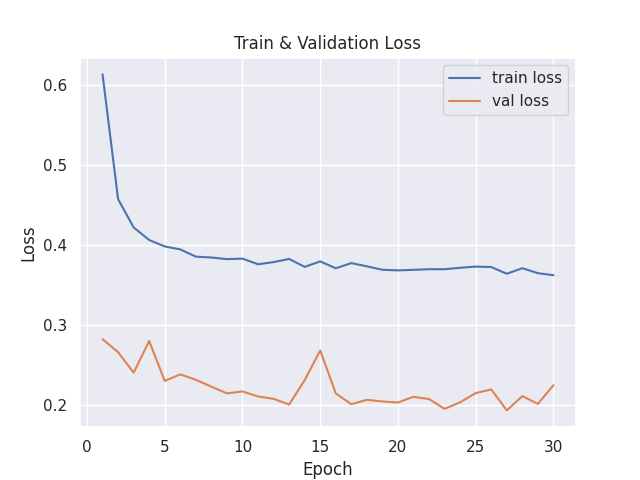
\includegraphics[ width=0.8\textwidth]{images/chapter experiments/method 3/romav/loss.png}
    \caption{Συνολικό σφάλμα μετρούμενο κατά την εκπαίδευση για τον αλγόριθμο \en{Multihead RoMAV} της 3\textsuperscript{ης} μεθόδου με αριθμό κεφαλών 2.}
    \label{fig:method3_romav}
  \end{figure}

\subsubsection{Πειραματικά Αποτελέσματα Αλγορίθμου \en{RoWSS} και \en{Multihead RoWSS}}

Συνεχίζοντας την πειραματική μελέτη της μεθόδου 3, επόμενος αλγόριθμος στην σειρά είναι ο \en{RoWSS} (αλγόριθμος \ref{alg:method3_max_routing}) και η πολυκέφαλη παραλλαγή του (αλγόριθμος \ref{alg:method3_max_multihead_routing}). Σε αυτούς τους αλγορίθμους, τα πειράματα είναι περισσότερα καθώς θέλουμε να εξετάσουμε, εκτός από τις υπερπαραμέτρους που πειράζαμε στην προηγούμενη παράγραφο, επιπέον υπερπαραμέτρους που δεν ήταν διαθέσιμοι στον προηγούμενο αλγόριθμο (εκ φύσεως). Αναλυτικότερα, αυτές οι παραλλαγές είναι η κλιμάκωση των εκπροσώπων με τις τιμές των αντίστοιχων σκορ ομοιότητας (\en{ScaleEMB}) αλλά και η εφαρμογή της συνάρτησης \en{Softmax} στα σκορ ομοιότητας (\en{SoftSC}) \footnote{Βλέπε αλγόριθμο \ref{alg:method3_max_routing} γραμμή \ref{op:method3_max_softmax_like_previous_softmax}.}.\par

Τα σχετικά πειράματα παρατίθενται στον πίνακα \ref{tab:method_3_hyper_tuning_RoWSS}. Σημειώνουμε ότι ορισμένα αποτελέσματα έχουν προκύψει από την χρήση εκθετικής μείωσης του ρυθμού μάθησης, καθώς μετά από πειράματα βρέθηκε πως συνέβαλε στην επίδοση\footnote{Θα ήταν αδύνατο να ενσωματώσουμε όλα τα πειράματα στο παρόν έργο. Σε περίπτωση που ορισμένα δε βρίσκονται στην \href{https://github.com/abarmper/Capsule_Nets_with_uncertainty}{ιστοσελίδα} του κώδικα, μπορούν να παρασχεθούν μετά από αίτημα μαζί με τα αρχεία βαρών των μοντέλων.}.\par

Από τα σχετικά αποτελέσματα είναι ασφαλές να υποθέσουμε ότι η κλιμάκωση των εκπροσώπων δεν βοηθάει την επίδοση του δικτύου. Εν αντιθέση, προκαλεί ακόμα μεγαλύτερη αστάθεια στο δίκτυο κατά την εκπαίδευση. Σε ό,τι αφορά τη χρήση της συνάρτησης \en{Softmax}, είναι εμφανές ότι δεν συνεπάγεται πάντα καλύτερη επίδοση. Με άλλα λόγια, η υπόθεση της ύπαρξης μοναδικού πατέρα (\en{single parent assumption}), όταν παραβαίνεται, μπορεί να οδηγήσει σε καλύτερα αποτελέσματα.\par

Αναφορικά με τον αριθμό των κεφαλών και το είδος του αποκωδικοποιητή, οι παρατηρήσεις είναι παρόμοιες με αυτές του αλγορίθμου \en{RoMAV}. Δηλαδή, και εδώ η αύξηση των κεφαλών γενικά οδηγεί σε καλύτερη επίδοση χωρίς ουσιαστική επιβάρυνση της πολυπλοκότητας. Βέβαια, αξίζει να σημειώσουμε ότι στην περίπτωση που ο αριθμός κεφαλών είναι ίσος με τη μονάδα, δεν παρατηρείται βελτίωση. Πιθανώς, αυτό οφείλεται στην επιπλέον πολυπλοκότητα που εισάγουν οι προβολές του διανύσματος και την τάση για υπερπροσαρμογή.\par 


\begin{table}[H]
    \begin{center}
        \en{
        \begin{tabular}{c c c c c c c c}
            \toprule
            Epoch (s) & Step (ms) & Param. & Heads & SoftSC & ScaleEmb & Recon. & Test Error (\%) \\ 
            \midrule
            35 & 11 & 151.8k & 0 & yes & no & FC & 1.9959 \\% 2.4074 % 9
            34 & 11 & 151.8k & 0 & no & no & FC & 1.9095\\ % 2.0412
            35 & 12 & 151.8k & 0 & yes & yes & FC & 3.0206 \\
            35 & 11 & 151.8k & 0 & no & yes & FC & 2.1564 \\

            45 & 15 & 151.8k & 0 & yes & no & Decon. & 1.7984 \\ %lrelu:1.8930<<-2.2675(1.8477)
            45 & 15 & 151.8k & 0 & no & no & Decon. & 1.7407 \\%<<-2.2798lrelu:1.8354(2.3498)(2.0165)
            46 & 15 & 151.8k & 0 & yes & yes & Decon. & 2.5885 \\
            45 & 15 & 151.8k & 0 & no & yes & Decon. & 2.8642 \\

            29 & 09 & 151.8k & 0 & yes & no & no & 2.1193 \\%lrelu:2.4403, <<-2.1193
            28 & 09 & 151.8k & 0 & no & no & no & \textbf{1.5309} \\%<<-2.7531
            29 & 10 & 151.8k & 0 & yes & yes & no & 2.3498 \\
            29 & 10 & 151.8k & 0 & no & yes & no & 2.2346 \\
            \midrule
            37 & 12 & 152.8k & 1 & yes & no & FC & 2.0741 \\%(θέλω μικρότερο του 1.99) <<-2.7778
            37 & 12 & 152.8k & 1 & no & no & FC & 2.1481\\%(θέλω μικρότερο του 2.04) 2.2881 <<-
            37 & 12 & 152.8k & 1 & yes & yes & FC & 2.8848 \\
            37 & 12 & 152.8k & 1 & no & yes & FC & 1.9218  \\

            48 & 16 & 152.8k & 1 & yes & no & Decon. & 2.1399\\%%(θέλω < του 1.79)\\ 2.7860 <<-
            48 & 16 & 152.8k & 1 & no & no & Decon. & 2.8930\\%(θέλω < του 1.74) 2.8971 <<-
            48 & 16 & 152.8k & 1 & yes & yes & Decon. & 2.2757 \\
            48 & 16 & 152.8k & 1 & no & yes & Decon. & 2.1152 \\

            31 & 10 & 152.8k & 1 & yes & no & no & 1.6626 \\%(θέλω μικρότερο του 1.53) <<- 1.7860
            31 & 10 & 152.8k & 1 & no & no & no & 1.5679 \\%%(θέλω μικρό) 2.0041 <<-
            31 & 10 & 152.8k & 1 & yes & yes & no & 2.0370 \\
            31 & 10 & 152.8k & 1 & no & yes & no & 2.9877 \\
            \midrule
            37 & 12 & 152.8k & 2 & yes & no & FC & 1.6626\\ %(θέλω < 1.99) 2.9712 <<-
            37 & 12 & 152.8k & 2 & no & no & FC & 1.5844\\%(θέλω < 2.04) 2.3909 <<-
            38 & 12 & 152.8k & 2 & yes & yes & FC & 2.8272 \\
            37 & 13 & 152.8k & 2 & no & yes & FC & 2.8313 \\

            48 & 16 & 152.8k & 2 & yes & no & Decon. & \textbf{1.5597} \\ % <<-2.1399
            48 & 16 & 152.8k & 2 & no & no & Decon. & 1.8807 \\ %(θέλω < του 1.74) <<- 2.2798
            49 & 16 & 152.8k & 2 & yes & yes & Decon. & 3.4774 \\
            49 & 16 & 152.8k & 2 & no & yes & Decon. & 2.1276  \\

            31 & 10 & 152.8k & 2 & yes & no & no & 1.8272 \\ % 2.5720 <<- %repeat
            31 & 10 & 152.8k & 2 & no & no & no & 1.7695\\ % <<-2.7037 %repeat
            31 & 10 & 152.8k & 2 & yes & yes & no & 2.5679 \\
            31 & 10 & 152.8k & 2 & no & yes & no & 2.3292 \\

            \bottomrule
        \end{tabular}
        }
    \end{center}
    \caption[]{\label{tab:method_3_hyper_tuning_RoWSS}Αποτελέσματα εκτενών πειραμάτων για την εύρεση των βέλτιστων υπερπαραμέτρων του αλγορίθμου \en{RoWSS} αρχιτεκτονικής \en{DepthConv} στο σύνολο δεδομένων \en{SmallNORB}. Πραγματοποιήθηκαν για 30 εποχές με μέγεθος δέσμης ίσο με 8.} 
\end{table}


Παρατηρούμε επιπλέον ότι η χρησιμότητα του δικτύου αποκωδικοποιητή είναι λιγότερο προφανής. Ένας πιθανός λόγος είναι ότι σε πολλές διατάξεις του αλγορίθμου η τιμή κλιμάκωσης του σφάλματος ανακατασκευής δεν είναι η κατάλληλη. Αυτό διότι το σφάλμα ανακατασκευής μετά την εκπαίδευση κυμαίνεται στις 1 με 2 μονάδες, ενώ το σφάλμα εκπαίδευσης είναι τρεις τάξεις μεγέθους χαμηλότερο (φυσικά και λόγο υπερπροσαρμογής). Συνεπώς, ακόμα και μετά την κλιμάκωση με τον όρο $0.2$, στις τελευταίες εποχές του αλγορίθμου, το σφάλμα αποκωδικοποιητή κυριαρχεί του σφάλματος κωδικοποιητή, γεγονός που δεν επιτρέπει την κατάλληλη προσαρμογή των βαρών. Επίσης, ο μικρός ανακατασκευαστής \en{Decon.} δεν επαρκεί για να ανακατασκευάσει την εικόνα εισόδου.\par

Στο σχήμα \ref{fig:method3_rowss} απεικονίζονται οι γραφικές παραστάσεις του σφάλματος στα σύνολα εκπαίδευσης και επαλήθευσης για το μοντέλο με την καλύτερη επίδοση (αυτό με μηδέν κεφαλές και χωρίς ανακατασκευαστή). 

\begin{figure}[h]
    \centering
    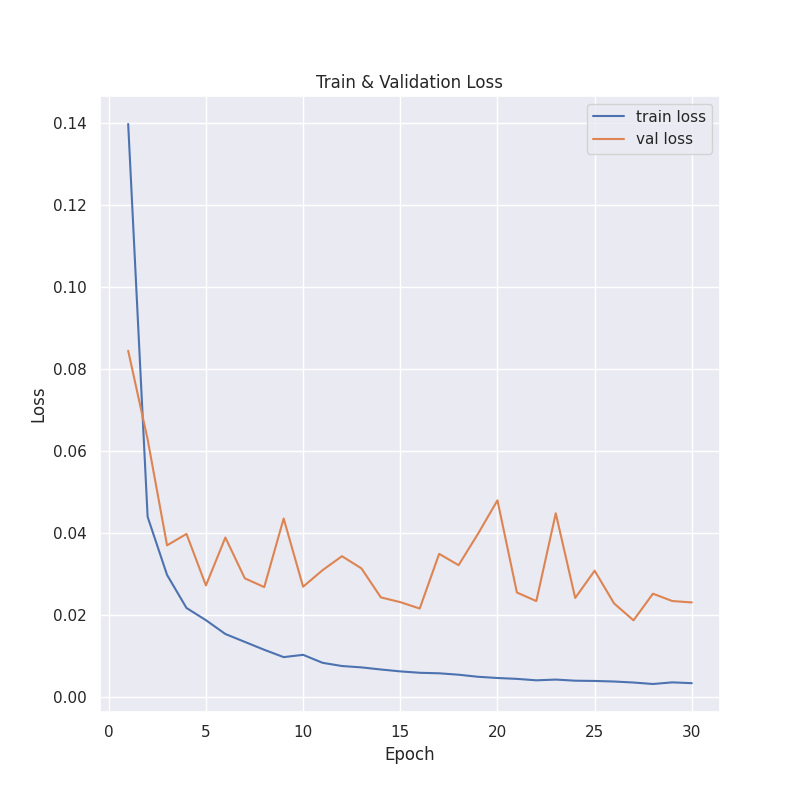
\includegraphics[ width=0.8\textwidth]{images/chapter experiments/method 3/rowss/loss.png}
    \caption{Συνολικό σφάλμα μετρούμενο κατά την εκπαίδευση για τον αλγόριθμο \en{RoWSS} της 3\textsuperscript{ης} μεθόδου. Εδώ δεν έχουμε ανακατασκευαστή. Για αυτό και το σφάλμα ελέγχου είναι μεγαλύτερο από το σφάλμα εκπαίδευσης.}
    \label{fig:method3_rowss}
\end{figure}

\subsubsection{Πειραματικά Αποτελέσματα Αλγορίθμων \en{RoWLS} και \en{Multihead RoWLS}}
Τελευταίος αλγόριθμος για τον οποίο θα κάνουμε αναζήτηση υπερπαραμέτρων για το σύνολο δεδομένων \en{SmallNORB} είναι ο \en{RoWLS} (αλγόριθμος \ref{alg:method3_max_len_routing}). Φυσικά, όπως και στα προειγούμενα πειράματα, όταν ο αριθμός κεφαλών είναι μεγαλύτερος από το μηδέν, υπονοείται ότι χρησιμοποιούμε τον αλγόριθμο \en{Multihead RoWLS} (αλγόριθμος \ref{alg:method3_max_len_multihead_routing}).\par

Οι παράμετροι που εξετάζουμε είναι οι ίδιες με αυτές του προηγούμενου πειράματος. Η διαφορά είναι ότι παρατηρώντας ότι η κλιμάκωση των \en{embeddings} με τα σκορ δεν συμβάλει στην επίδοση του αλγορίθμου \en{RoWLS}, μειώσαμε τα πειράματα και για τον αλγόριθμο \en{Multihead RoWLS} εξετάσαμε μόνο την περίπτωση όπου δεν πραγματοποιείται η σχετική κλιμάκωση. Τα αποτελέσματα των πειραμάτων παρατίθενται στον πίνακα \ref{tab:method_3_hyper_tuning_RoWLS}.

\begin{table}[H]
    \begin{center}
        \en{
        \begin{tabular}{c c c c c c c c}
            \toprule
            Epoch (s) & Step (ms) & Param. & Heads & SoftSC & ScaleEmb & Recon. & Test Error (\%) \\ 
            \midrule
            34 & 11 & 151.8k & 0 & yes & no & FC &  2.3992 \\% 
            34 & 11 & 151.8k & 0 & no & no & FC & 2.2757 \\
            35 & 12 & 151.8k & 0 & yes & yes & FC & 2.2881 \\
            35 & 11 & 151.8k & 0 & no & yes & FC & 2.2593 \\

            45 & 15 & 151.8k & 0 & yes & no & Decon. & 2.5103 \\ % <<-2.5597
            45 & 15 & 151.8k & 0 & no & no & Decon. & 1.7613 \\% <<-2.0535
            46 & 15 & 151.8k & 0 & yes & yes & Decon. & 2.3868 \\
            45 & 15 & 151.8k & 0 & no & yes & Decon. & 2.2263 \\

            29 & 09 & 151.8k & 0 & yes & no & no & 1.7942\\% 2.0658 <<-
            28 & 09 & 151.8k & 0 & no & no & no & 1.6831\\% 1.8107 <<-
            29 & 10 & 151.8k & 0 & yes & yes & no & 2.2675 \\% 20.5
            29 & 10 & 151.8k & 0 & no & yes & no & 2.5597 \\% 20.75

            37 & 12 & 152.8k & 1 & yes & no & FC & 2.4280 \\% 21.0
            37 & 12 & 152.8k & 1 & no & no & FC & 2.0658 \\%

            48 & 16 & 152.8k & 1 & yes & no & Decon. & 2.8272 \\%
            48 & 16 & 152.8k & 1 & no & no & Decon. & 1.8477 \\%

            31 & 10 & 152.8k & 1 & yes & no & no & 2.1235 \\%
            31 & 10 & 152.8k & 1 & no & no & no & 2.1523 \\%

            37 & 12 & 152.8k & 2 & yes & no & FC & 2.6996 \\ % 
            37 & 12 & 152.8k & 2 & no & no & FC & 2.1317 \\% 

            48 & 16 & 152.8k & 2 & yes & no & Decon. & 2.2058 \\ % <<-2.7160
            48 & 16 & 152.8k & 2 & no & no & Decon. & \textbf{1.5967}\\ %2.2675 <<-

            31 & 10 & 152.8k & 2 & yes & no & no & \textbf{1.5021}\\% 2.2099 <<- 
            31 & 10 & 152.8k & 2 & no & no & no & 2.1276\\%

            \bottomrule
        \end{tabular}
        }
    \end{center}
    \caption[]{\label{tab:method_3_hyper_tuning_RoWLS}Αποτελέσματα πειραμάτων για την εύρεση των βέλτιστων υπερπαραμέτρων του αλγορίθμου \en{RoWLS} αρχιτεκτονικής \en{DepthConv} στο σύνολο δεδομένων \en{SmallNORB}. Όλα τα πειράματα της ενότητας πραγματοποιήθηκαν για 30 εποχές με μέγεθος δέσμης ίσο με 8.} 
\end{table}
Παρατηρούμε ότι τα αποτελέσματα αν και είναι πολύ ικανοποιητικά, σε γενικές γραμμές φαίνεται ότι η μέθοδος \en{RoWSS} υπερτερεί της μεθόδου \en{RoWLS} (πλην λίγων εξαιρέσεων). Το γεγονός αυτό συνεπάγεται ότι το κριτήριο επιλογής εκπροσώπων με βάση τη συμφωνία είναι συνήθως καλύτερο από το κριτήριο του μήκους των αναπαραστάσεων (\en{embeddings}).\par

Σχετικά με τον ανακατασκευαστή, είναι αξιοσημείωτο πως και πάλι, το μοντέλο με τις καλύτερες παραμέτρους είναι ένα χωρίς ανακατασκευαστή. Είναι λοιπόν πιθανό ότι το σφάλμα ανακατασκευής είναι μεγαλύτερο από αυτό που θα έπρεπε στα συγκεκριμένα πειράματα (ή ότι ο ανακατασκευαστής δεν είναι κατάλληλος). Στις εικόνες \ref{fig:method3_rowls_left} και \ref{fig:method3_rowls_right} αντιπαραβάλλονται τα σφάλματα από τον κωδικοποιητή (αριστερά) και τον αποκωδικοποιητή (δεξιά). Βλέπουμε ότι το σφάλμα της ανακατασκευής είναι δύο κλάσεις μεγέθους μεγαλύτερο του σφάλματος \en{margin loss}. Επίσης, βλέπουμε ότι το σφάλμα ελέγχου για την ανακατασκευή είναι μικρότερο από το σφάλμα στο σύνολο εκπαίδευσης. Όπως έχουμε εξηγήσει, αυτό οφείλεται στην πιο έντονη επαύξηση δεδομένων που χρησιμοποιούμε για το σύνολο εκπαίδευσης.

\begin{figure}
    \centering
    \begin{minipage}{.5\textwidth}
      \centering
      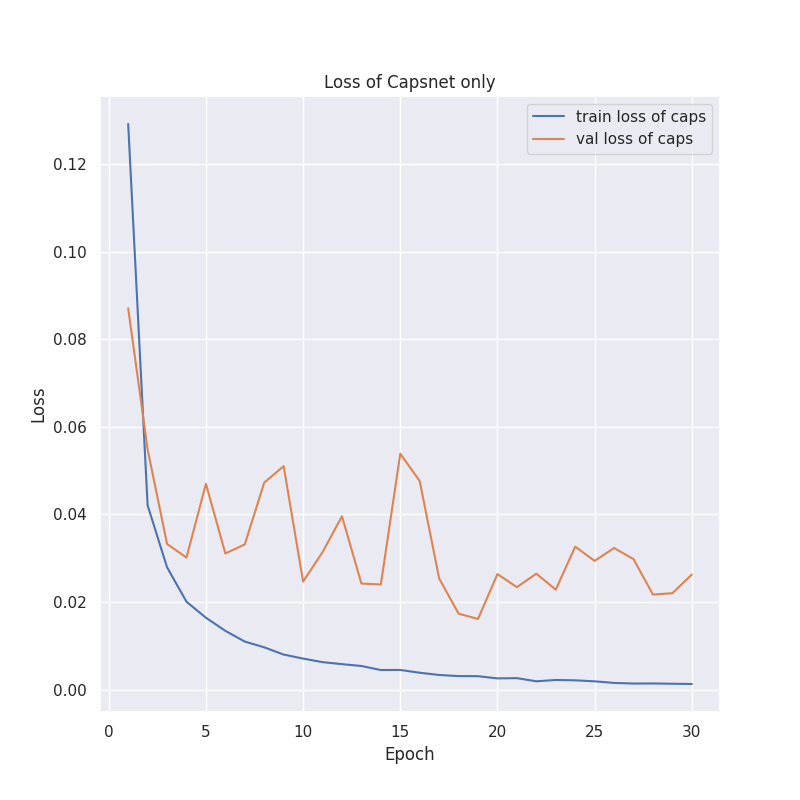
\includegraphics[trim={2cm 0 2cm 0},clip,width=.65\linewidth]{images/chapter experiments/method 3/rowls/loss_only_capsnet_good.png}
      \captionsetup{width=0.8\linewidth}
      \captionof{figure}{Σφάλμα κωδικοποιητή (αλγόριθμος \en{RoWLS}).}
      \label{fig:method3_rowls_left}
    \end{minipage}%
    \begin{minipage}{.45\textwidth}
      \centering
      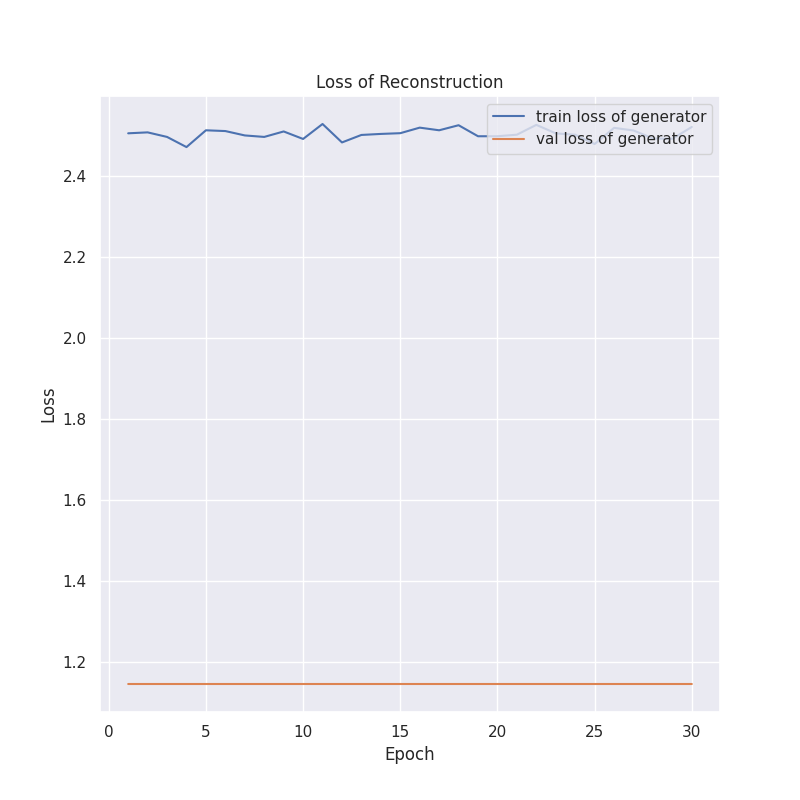
\includegraphics[trim={2cm 0 2cm 0},clip,width=.73\linewidth]{images/chapter experiments/method 3/rowls/loss_only_reconstruction_good.png}
      \captionsetup{width=0.8\linewidth}
      \captionof{figure}{Σφάλμα αποκωδικοποιητή (αλγόριθμος \en{RoWLS}).}
      \label{fig:method3_rowls_right}
    \end{minipage}
    \end{figure}

\subsection{Πειράματα Παραμέτρου Ανακατασκευής}

Προκειμένου να εξεταστεί αν χαμηλότερη τιμή της παραμέτρου κλιμάκωσης του σφάλματος ανακατασκευής οδηγεί σε καλύτερα αποτελέσματα, διενεργούμε πείραμα στο μοντέλο του αλγορίθμου (\en{RoWSS}). Χρησιμοποιούμε την παραμετροποίηση που του εξασφαλίζει \en{test error} \textbf{1.5597} αλλά με πιο έντονη κλιμάκωση του σφάλματος ανακατασκευής (τιμές $0.02$ και $0.0005$). Τα πειράματα πραγματοποιούνται και πάλι για 30 εποχές με μέγεθος δέσμης ίσο με 8. Παρατίθενται στον πίνακα \ref{tab:method_3_hyper_tuning_scaling_factor}.


\begin{table}[h]
    \begin{center}
        \en{
        \begin{tabular}{c c c}
            \toprule
            Scaling Factor  & Recon. (type) & Test Error (\%) \\ 
            \midrule
            0.2 & yes (Decon.) &  \textbf{1.5597} \\
            0.02 &  yes (Decon.) &  2.3004 \\
            0.005 & yes (Decon.) &  1.8889 \\
            \bottomrule
        \end{tabular}
        }
    \end{center}
    \caption[]{\label{tab:method_3_hyper_tuning_scaling_factor}Αποτελέσματα πειραμάτων για την εύρεση της βέλτιστης τιμής του παράγοντα κλιμάκωσης του σφάλματος ανακατασκευής στο σύνολο δεδομένων \en{SmallNORB}. Τα πειράματα πραγματοποιήθηκαν για 30 εποχές με μέγεθος δέσμης ίσο με 8.} 
\end{table}

Από τα σχετικά πειράματα, δεν φαίνεται να υπάρχει κάποια βελτίωση με την μείωση της τιμής της παραμέτρου. Για τον λόγο αυτό, στα πειράματα εμβάθυνσης, αφήνουμε την υπερπαράμετρο στην προκαθορισμένη της τιμή η οποία έχει προσφέρει αξιοσημείωτα αποτελέσματα σε όλους τους αλγορίθμους της τρίτης μεθόδου.

\subsection{Επιλεκτική Εμβάθυνση στα Σύνολα Δεδομένων}
Σε αυτήν την ενότητα, επιλέγουμε από τον κάθε τύπο αλγορίθμου (\en{RoMAV, RoWSS, RoWLS}) τα μοντέλα με τις δύο παραμετροποιήσεις που οδήγησαν στα καλύτερα αποτελέσματα στο σύνολο δεδομένων \en{SmallNORB} και τα εκπαιδεύουμε σε μια πληθώρα από σύνολα δεδομένων\footnote{Είναι γεγονός ότι οι παράμετροι που δουλεύουν για ένα σύνολο δεδομένων μπορεί να μην είναι οι καλύτεροι για κάποιο άλλο σύνολο.}. Ουσιαστκά, για τους αλγορίθμους (\en{RoMAV, RoWSS, RoWLS}) έχουμε δύο μοντέλα, ένα με ανακατασκευή και ένα χωρίς. Σημειώνουμε ότι όλα τα πειράματα γίνονται για 30 εποχές.\par

\subsubsection{Σύνολο Δεδομένων \en{MNIST}}

Τα αποτελέσματα των πειραμάτων για το πρόβλημα \en{MNIST} παρουσιάζονται στον πίνακα \ref{tab:method_3_MNIST_final}. Χρησιμοποιούμε μέγεθος δέσμης 32 και παράγοντα κλιμάκωσης σφάλματος ίσο με $0.05$ διότι από επιπλέον πειράματα φάνηκε ότι αυτή η τιμή είναι καταλληλότερη για το εν λόγο \en{dataset}. Στον πίνακα αποτελεσμάτων αναγράφεται και η εφαρμογή ή μη της συνάρτησης ομαλής μεγιστοποίησης που συνεπάγεται την τήρηση ή μη της υπόθεσης μοναδικού πατέρα (παράμετρος \en{SoftSC}). Συμπληρωματικά αναφέρεται ότι ο αριθμός των παραμέτρων του αποκωδικοποιητή από επίπεδα αποσυνέλιξης (όπου χρησιμοποιείται) είναι $250.1k$.

\begin{table}[h]
    \begin{center}
        \en{
        \begin{tabular}{c c c c c c}
            \toprule
            Algorithm & SoftSC & Heads & Param. Count & Reconstruction & Test Error (\%) \\ 
            \midrule
            RoMAV & - & 2 & 162.7 & yes (Decon.) & 0.34 \\
            RoMAV & - & 2 & 162.7 & yes (FC) & \textbf{0.30*} \\
            RoMAV & - & 2 & 162.7 & no & 0.36 \\
            RoWSS & yes & 2 & 162.7 & yes (Decon.) & 0.36 \\
            RoWSS & no & 2 & 162.7 & no & 0.37 \\
            RoWLS & no & 2 & 162.7 & yes (Decon.) & 0.38 \\
            RoWLS & yes & 2 & 162.7 & no & 0.34 \\
            \bottomrule
        \end{tabular}
        }
    \end{center}
    \caption[]{\label{tab:method_3_MNIST_final}Επίδοση των αλγορίθμων της μεθόδου 3 στο σύνολο δεδομένων \en{MNIST}, όταν χρησιμοποιούνται 30 εποχές για την εκπαίδευση του μοντέλου με μέγεθος δέσμης 32. Το αποτέλεσμα με αστερίσκο προέκυψε μετά από 60 εποχές.} 
\end{table}

Παρατηρούμε ότι τα αποτελέσμτατα είναι πολύ ικανοποιητικά (όπως θα δούμε και στο τέλος του κεφαλαίου όπου θα γίνει σύγκριση με άλλα συστήματα που συναντώνται στη βιβλιογραφία). Συγκρίνοντας τους αλγορίθμους της μεθόδου 3 μεταξύ τους, μπορούμε με ασφάλεια να ισχυριστούμε ότι η επίδοση των αλγορίθμων μας στο συγκεκριμένο πρόβλημα είναι παραπλήσια. \par

Στο συγκεκριμένο \en{dataset} χρησιμοποιούμε αρκετά μεγαλύτερο σύνολο δέσμης επειδή το μέγεθος της μνήμης τυχαίας προσπέλασης του επιταχυντή μας το επιτρέπει. Παρατηρήσαμε πολύ πιο σταθερή σύγκλιση και σχεδόν μηδενικές περιπτώσεις αστάθειας\footnote{Σε ορισμένες περιπτώσεις μεγάλης αστάθειας, το σφάλμα γίνεται \en{not-a-number} και το πείραμα πρέπει να επαναληφθεί.}.

\subsubsection{Σύνολο Δεδομένων \en{Fashion-MNIST}}

Σχετικά με τα πειράματα για το \en{Fashion-MNIST}, τα πορίσματά τους αναγράφονται στον πίνακα \ref{tab:method_3_FashionMNIST_final}. Χρησιμοποιούμε μέγεθος δέσμης 32 και παράγοντα κλιμάκωσης σφάλματος ίσο με $0.05$. Ο αριθμός των παραμέτρων του αποκωδικοποιητή από επίπεδα αποσυνέλιξης (όπου χρησιμοποιείται) είναι $250.1k$.

\begin{table}[h]
    \begin{center}
        \en{
        \begin{tabular}{c c c c c c}
            \toprule
            Algorithm & SoftSC & Heads & Param. Count & Reconstruction & Test Error (\%) \\ 
            \midrule
            RoMAV & - & 2 & 162.7 & yes (Decon.) & 8.22 \\ % 1
            RoMAV & - & 2 & 162.7 & no & \textbf{7.84} \\
            RoWSS & yes & 2 & 162.7 & yes (Decon.) & 8.43 \\
            RoWSS & no & 2 & 162.7 & no & 8.38 \\
            RoWLS & no & 2 & 162.7 & yes (Decon.) & 8.32 \\
            RoWLS & yes & 2 & 162.7 & no & 7.87 \\ % 6
            \bottomrule
        \end{tabular}
        }
    \end{center}
    \caption[]{\label{tab:method_3_FashionMNIST_final}Επίδοση των αλγορίθμων της μεθόδου 3 στο σύνολο δεδομένων \en{Fashion-MNIST}, όταν χρησιμοποιούνται 30 εποχές για την εκπαίδευση του μοντέλου με μέγεθος δέσμης 32.} 
\end{table}

Παρατηρούυμε ότι τα αποτελέσματα είναι και εδώ πολύ ικανοποιητικά μιας και όπως θα δούμε στην συνέχεια, χωρίς καμία αναζήτηση βέλτιστων παραμέτρων για το συγκεκριμένο \en{dataset}, ο αλγόριθμός μας είναι ανάμεσα στους καλύτερους σύμφωνα με αυτή τη \href{https://paperswithcode.com/sota/image-classification-on-fashion-mnist}{λίστα}.\par

Σημειώνουμε ότι η επίδοση μπορεί να βελτιωθεί με την αύξηση των εποχών αφού από το σύνολο \en{validation} φαίνονταν να συνεχίζει να αυξάνεται η επίδοση στις τελευταίες εποχές.

\subsubsection{Σύνολο Δεδομένων \en{MultiMNIST}}

Τα πειραματικά αποτελέσματα για το σύνολο δεδομένων \en{MultiMNIST} εμφανίζονται στον πίνακα \ref{tab:method_3_MultiMNIST_final}. Έχουμε αυτή τη φορά μέγεθος δέσμης 64 και παράγοντα κλιμάκωσης σφάλματος ανακατασκευής ίσο με $0.05$. Συμπληρωματικά αναφέρεται και πάλι ότι ο αριθμός των παραμέτρων του αποκωδικοποιητή από επίπεδα αποσυνέλιξης (όπου χρησιμοποιείται) είναι $353.1k$.

\begin{table}[h]
    \begin{center}
        \en{
        \begin{tabular}{c c c c c c}
            \toprule
            Algorithm & SoftSC & Heads & Param. Count & Reconstruction & Test Error (\%) \\ 
            \midrule
            RoMAV & - & 2 & 156.9 & yes (Decon.) & \textbf{6.2115} \\ % 7 (not inclued)
            RoMAV & - & 2 & 156.9 & no & 6.2615 \\ % 8 (not inclued)
            RoWSS & yes & 2 & 156.9 & yes (Decon.) & 6.6670 \\
            RoWSS & no & 2 & 156.9 & no & 7.2555 \\
            RoWLS & no & 2 & 156.9 & yes (Decon.) & 6.7500 \\
            RoWLS & yes & 2 & 156.9 & no & 6.4050 \\ % 12
            \bottomrule
        \end{tabular}
        }
    \end{center}
    \caption[]{\label{tab:method_3_MultiMNIST_final}Επίδοση των αλγορίθμων της μεθόδου 3 στο σύνολο δεδομένων \en{MultiMNIST}, όταν χρησιμοποιούνται 30 εποχές για την εκπαίδευση του μοντέλου με μέγεθος δέσμης 64.} 
\end{table}

Αν και η επίδοση δεν είναι καλύτερη από αυτή που εντοπίζεται στη βιβλιογραφία, το γεγονός ότι επιτυγχάνει ένα τόσο χαμηλό ποσοστό σφάλματος συνεπάγεται ότι το δίκτυό μας είναι εύρωστο στην αναγνώριση επικαλυπτόμενων ψηφίων, μια χαρακτηριστική ιδιότητα των νευρωνικών δικτύων με κάψουλες. Με άλλα λόγια, αποδεικνύεται ότι κάθε κάψουλα του τελευταίου επιπέδου μπορεί να λειτουργήσει ανεξάρτητα και να συλάβει το στυλ και την θέση του ψηφίου που αναπαριστά από τις ψήφους που εκλαμβάνει.

\subsubsection{Σύνολο Δεδομένων \en{CIFAR10}}

Τα αποτελέσματα των πειραμάτων για το πιο σύνθετο πρόβλημα \en{CIFAR10} παρουσιάζονται στον πίνακα \ref{tab:method_3_CIFAR10_final}. Χρησιμοποιούμε μέγεθος δέσμης 32 και παράγοντα κλιμάκωσης σφάλματος ίσο με $0.05$. Επίσης, ακολουθώντας το έργο \cite{sabour2017dynamic} προσθέσαμε την κατηγορία \textquote{κανένα από τα παραπάνω}. Συμπληρωματικά αναφέρεται ότι ο αριθμός των παραμέτρων του αποκωδικοποιητή από επίπεδα αποσυνέλιξης (όπου χρησιμοποιείται) είναι $141.7k$.

\begin{table}[h]
    \begin{center}
        \en{
        \begin{tabular}{c c c c c c}
            \toprule
            Algorithm & SoftSC & Heads & Param. Count & Reconstruction & Test Error (\%) \\ 
            \midrule
            RoMAV & - & 2 & 265.2 & yes (Decon.) & \textbf{28.85} \\ %% 13
            RoMAV & - & 2 & 265.2 & no & 29.74 \\
            RoWSS & yes & 2 & 265.2 & yes (Decon.) & 30.01 \\
            RoWSS & no & 2 & 265.2 & no & 30.72 \\
            RoWLS & no & 2 & 265.2 & yes (Decon.) & 28.96 \\
            RoWLS & yes & 2 & 265.2 & no & 30.66 \\ % 18
            \bottomrule
        \end{tabular}
        }
    \end{center}
    \caption[]{\label{tab:method_3_CIFAR10_final}Επίδοση των αλγορίθμων της μεθόδου 3 στο σύνολο δεδομένων \en{CIFAR10}, όταν χρησιμοποιούνται 30 εποχές για την εκπαίδευση του μοντέλου με μέγεθος δέσμης 32.} 
\end{table}

Το συγκεκριμένο σύνολο δεδομένων είναι το πιο σύνθετο που δοκιμάζουμε. Είναι γεγονός ότι τα νευρωνικά δίκτυα από κάψουλες δεν ανταποκρίνονται καλά στο συγκεκριμένο σύνολο. Σε σχέση με άλλους αλγορίθμους της ίδιας τεχνολογίας, η επίδοση είναι χαμηλή (όπως θα δούμε στη συνέχεια). Αυτή η χαμηλή επίδοση μπορεί να προκύπτει από τρείς λόγους (με σειρά προτεραιότητας):
\begin{itemize}
    \item Μικρός αριθμός εποχών. Στις 30 εποχές παρατηρούνταν ακόμα βελτίωση επίδοσης.
    \item Απουσία μεθόδων για την μετρίαση του προβλήματος της υπερπροσαρμογής (\en{regulariation methods}).
    \item Χαμηλός αριθμός παραμέτρων δικτύου.
\end{itemize}

\subsubsection{Σύνολο Δεδομένων \en{SmallNORB}}

Για λόγους πληρότητας, παραθέτουμε τα αποτελέσματα που αφορούν το πρόβλημα \en{SmallNORB}, όπως προέκυψαν στην προηγούμενη υπο-ενότητα στον πίνακα \ref{tab:method_3_SmallNORB_final}. Υπενθυμίζεται ότι το μέγεθος δέσμης είναι 8 ενώ ο παράγοντας κλιμάκωσης σφάλματος ανακατασκευής ίσος με $0.2$. Υπενθυμίζεται επίσης ότι ο αριθμός των παραμέτρων του αποκωδικοποιητή από επίπεδα αποσυνέλιξης (όπου χρησιμοποιείται) είναι $229.5k$.

\begin{table}[h]
    \begin{center}
        \en{
        \begin{tabular}{c c c c c c}
            \toprule
            Algorithm & SoftSC & Heads & Param. Count & Reconstruction & Test Error (\%) \\ 
            \midrule
            RoMAV & - & 2 & 152.8 & yes (Decon.) & \textbf{1.4403} \\
            RoMAV & - & 2 & 152.8 & no & 1.5761 \\
            RoWSS & yes & 2 & 152.8 & yes (Decon.) & 1.5309 \\
            RoWSS & no & 2 & 152.8 & no & 1.5597 \\
            RoWLS & no & 2 & 152.8 & yes (Decon.) & 1.5967 \\
            RoWLS & yes & 2 & 152.8 & no & 1.5021 \\
            \bottomrule
        \end{tabular}
        }
    \end{center}
    \caption[]{\label{tab:method_3_SmallNORB_final}Επίδοση των αλγορίθμων της μεθόδου 3 στο σύνολο δεδομένων \en{SmallNORB}, όταν χρησιμοποιούνται 30 εποχές για την εκπαίδευση του μοντέλου με μέγεθος δέσμης 8.} 
\end{table}

\subsubsection{Συγκεντρωτικά Αποτελέσματα για Όλα τα Σύνολα Δεδομένων}
Για λόγους πληρότητας, παρουσιάζουμε στον πίνακα \ref{tab:method_3_all} για κάθε σύνολο δεδομένων τον αλγόριθμο της τρίτης μεθόδου που εμφάνισε τα καλύτερα αποτελέσματα (με και χωρίς ανακατασκευαστή).

\begin{table}[h]
    \begin{center}
        \en{
        \begin{tabular}{c c c c c c c}
            \toprule
            Dataset & Algorithm & SoftSC & Heads & Parameters (k) & Recon. & Test Error (\%) \\ 
            \midrule
            SmallNORB & RoMAV & - & 2 & 152.8 & Decon. & \textbf{1.4403} \\
            SmallNORB & RoMAV & - & 2 & 152.8 & no & 1.5761 \\
            \midrule
            MNIST & RoMAV & - & 2 & 162.7 & FC & \textbf{0.30} \\
            MNIST & RoWLS & yes & 2 & 162.7 & no & 0.34 \\
            \midrule
            Multi-MNIST & RoMAV & - & 2 & 156.9 & Decon. & \textbf{6.2115} \\
            Multi-MNIST & RoMAV & - & 2 & 156.9 & no & 6.2615 \\
            \midrule
            Fashion-MNIST & RoMAV & - & 2 & 162.7 & Decon. & 8.22 \\
            Fashion-MNIST & RoMAV & - & 2 & 162.7 & no & \textbf{7.84} \\
            \midrule
            CIFAR10 & RoMAV & - & 2 & 265.2 & Decon. & \textbf{28.85} \\
            CIFAR10 & RoMAV & - & 2 & 265.2 & no & 29.74 \\
            \bottomrule
        \end{tabular}
        }
    \end{center}
    \caption[]{\label{tab:method_3_all}Οι επιδόσεις των καλύτερων αλγορίθμων της μεθόδου 3 για το κάθε σύνολο δεδομένων.} 
\end{table}

\subsection{Ειδικά Πειράματα}
Οι αλγόριθμοι της μεθόδου 3 εμφανίζουν εξαιρετικά αποτελέσματα σε όλα τα σχετικά με τις κάψουλες σύνολα δεδομένων. Το γεγονός αυτό μας προδιαθέτει να πιστέψουμε πως πράγματι, πραγματοποιούν κατά μια έννοια \textquote{ανάστροφα γραφικά} και επιτυγχάνουν να αποσυνθέσουν την εικόνα σε εύρωστους παράγοντες συνδιακύμανσης (\en{factors of variation}).\par

Παρακινούμενοι από την επιθυμία μας να αποδείξουμε έμπρακτα την δυνατότητα των αλγορίθμων μας να αποκωδικοποιούν την εικόνα\footnote{Εικόνα από το σύνολο δεδομένων \en{MNIST}} εισόδου σε παραμέτρους στιγμιοτύπου όπως η πόζα και το στύλ, εφαρμόσαμε πειράματα διαταραχής (\en{perturbation}) στους αλγορίθμους \en{Multihead RoMAV} και \en{Multihead RoWSS} αφού εκπαιδεύτηκαν για 60 εποχές με την χρήση πλήρως διασυνεδεμένου αποκωδικοποιητή.\par

Τα αποτελέσματα και στις δύο περιπτώσεις ήταν πολύ ενθαρρυντικά. Για παράδειγμα, στην εικόνα \ref{fig:method3_pb_romav} φαίνεται τόσο η αρχική εικόνα όσο και η ανακατασκευασμένη εικόνα από το δίκτυο \en{RoMAV}. Στην επόμενη εικόνα, την \ref{fig:method3_pb_romav_2} φαίνεται πως μεταβάλλεται το ψηφίο εφτά αν μεταβάλουμε ελαφρώς τις παραμέτρους της αντίστοιχης κάψουλας.\par
\begin{figure}[h]
    \centering
    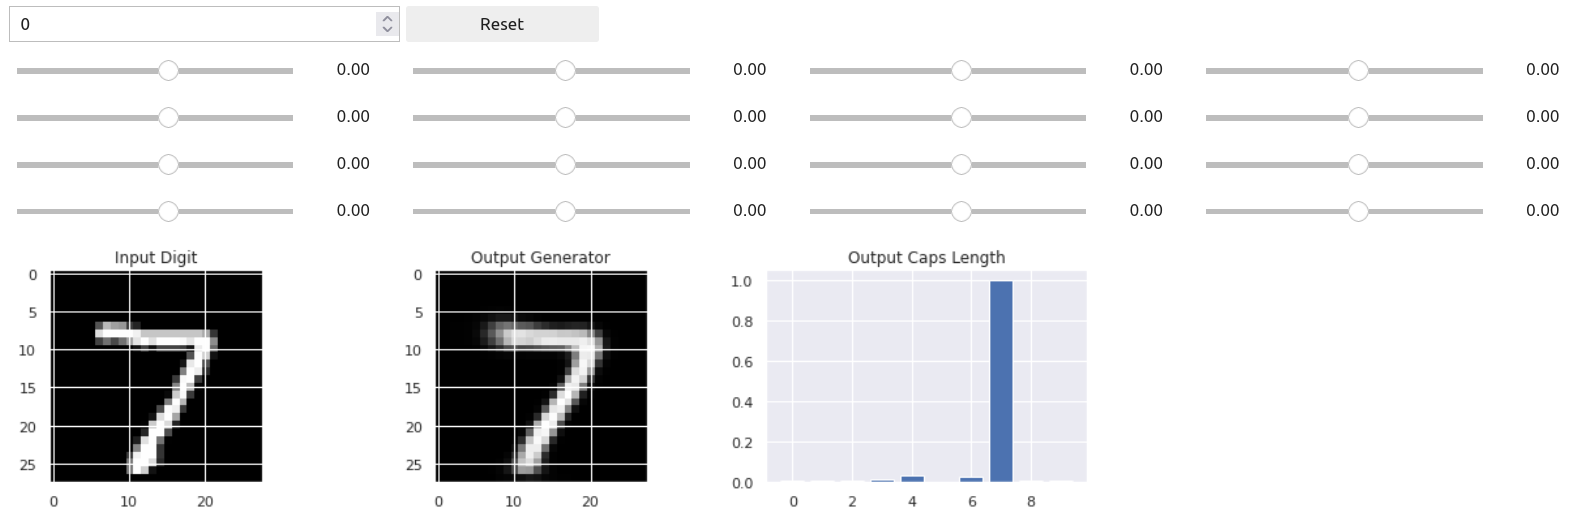
\includegraphics[ width=0.99\textwidth]{images/chapter experiments/method 3/perturbations_romav/perturbations_method3_roomav.png}
    \caption{Ανακατασκευασμένη εικόνα αλγορίθμου \en{Multihead RoMAV} με \en{FC} ανακατασκευαστή.}
    \label{fig:method3_pb_romav}
\end{figure}
\begin{figure}[h]
    \centering
    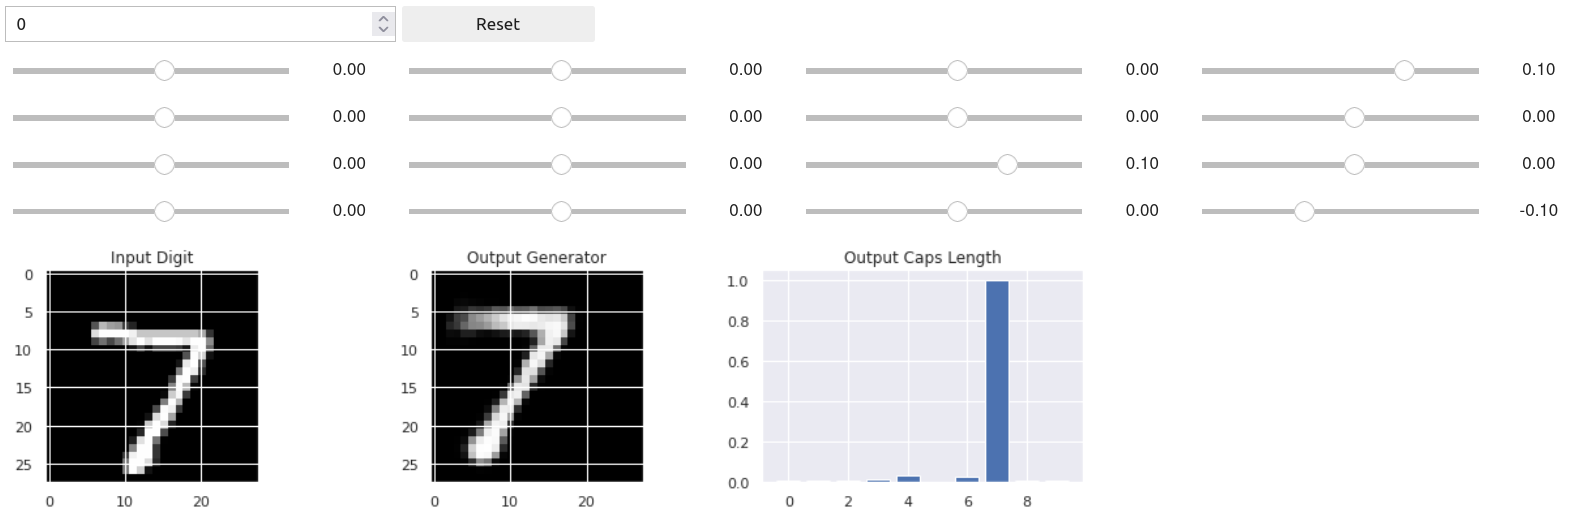
\includegraphics[ width=0.99\textwidth]{images/chapter experiments/method 3/perturbations_romav/perturbations_method3_roomav_2.png}
    \caption{Πείραμα διαταραχής αλγορίθμου \en{Multihead RoMAV} mμε \en{FC} ανακατασκευαστή.}
    \label{fig:method3_pb_romav_2}
\end{figure}

Αντίστοιχα για τον αλγόριθμο \en{RoWSS}, στην εικόνα \ref{fig:method3_pb_rowss} παρουσιάζεται το πείραμα διαταραχής για το ψηφίο δύο. Επίσης πραγματοποιήσαμε πειράματα με αποκωδικοποιητή με επίπεδα αποσυνέλιξης που διαθέτει πολύ λιγότερες παραμέτρους (περίπου 250\en{k}) αλλά φαίνεται να αδυνατεί να ανακατασκευάσει καλά την εικόνα και να μην βοηθάει στην αποδόμηση της εικόνας του κωδικοποιητή.

\begin{figure}[h]
    \centering
    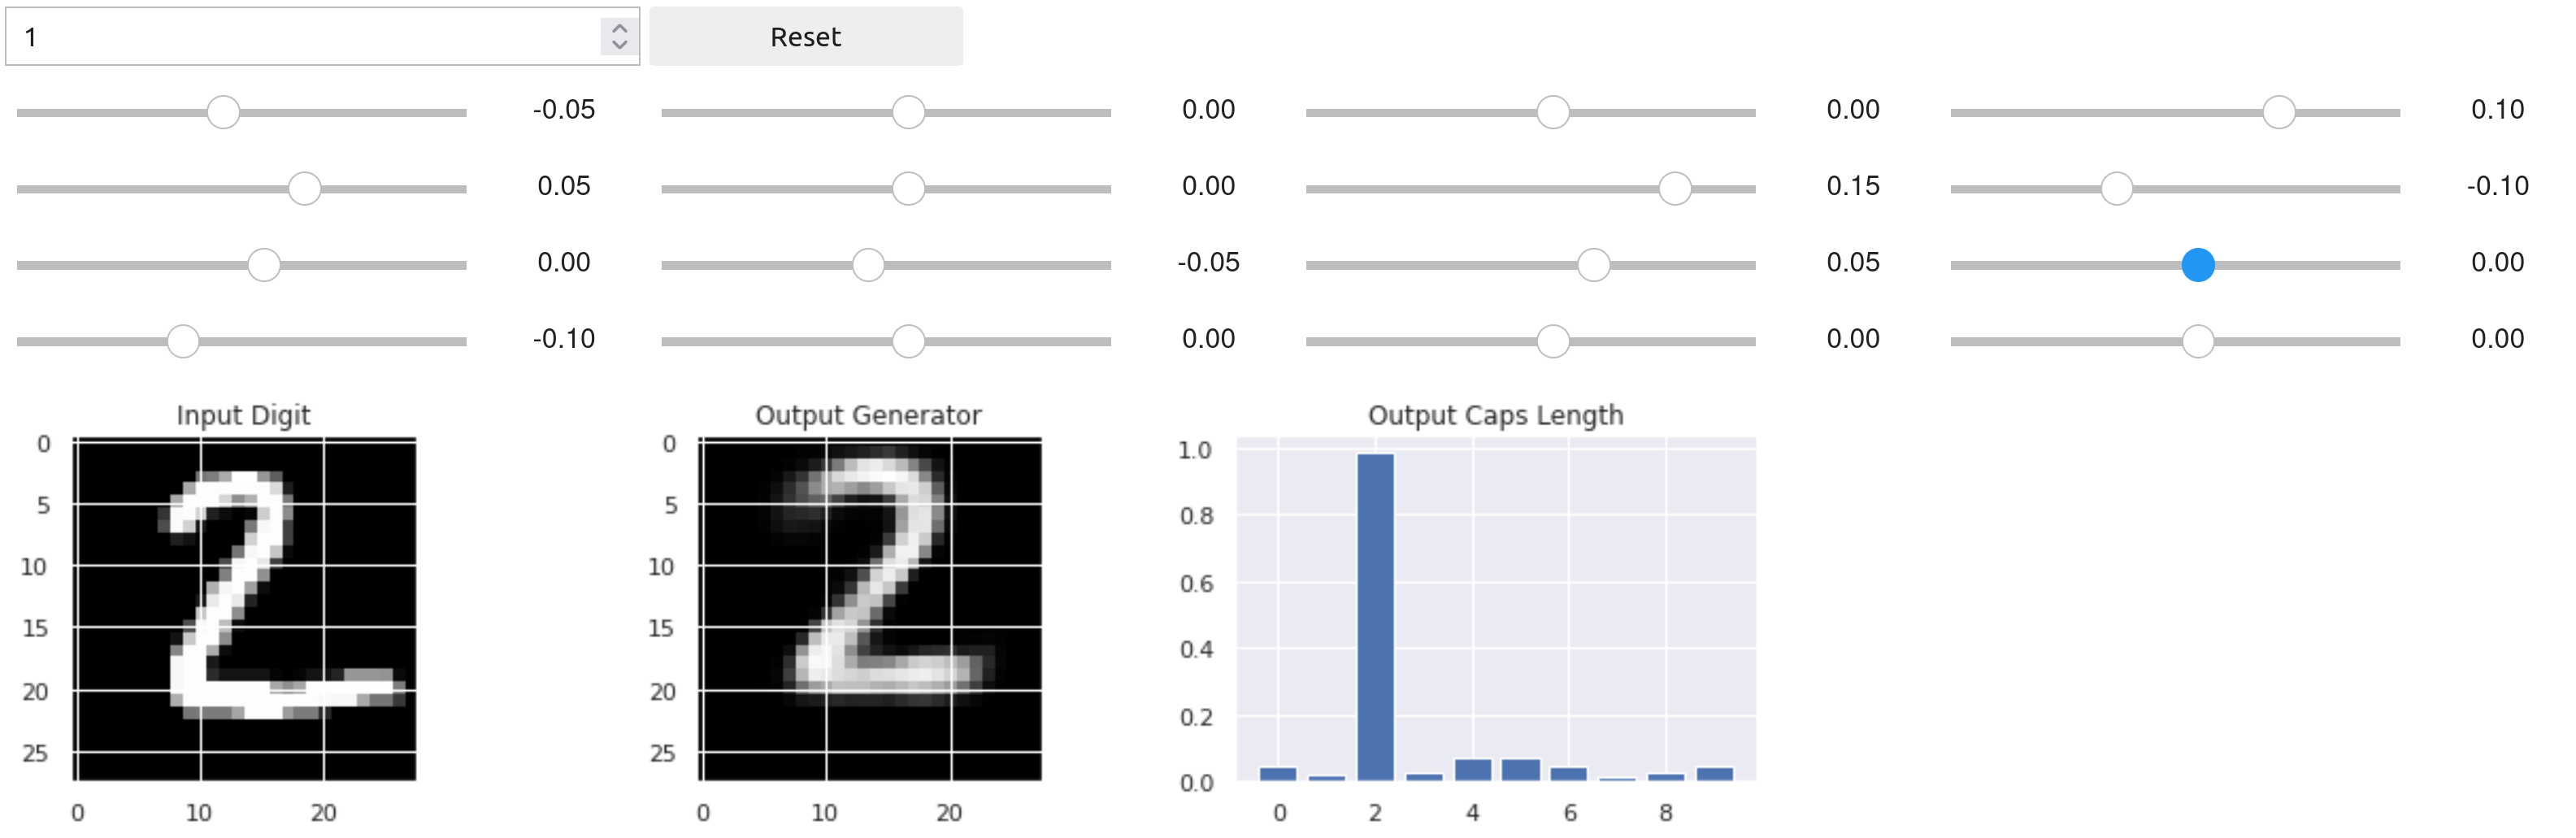
\includegraphics[ width=0.99\textwidth]{images/chapter experiments/method 3/pbatons_rowss/perturbations_rowss_2.png}
    \caption{Πείραμα διαταραχής αλγορίθμου \en{Multihead RoWSS} με \en{FC} ανακατασκευαστή.}
    \label{fig:method3_pb_rowss}
\end{figure}

\section{Πειραματική Μελέτη Μεθόδου 4}
 
Η τελευταία μέθοδος για την οποία πραγματοποιούμε πειράματα είναι η μέθοδος 4 που αφορά την οικογένεια αλγορίθμων υπό το όνομα \textquote{Αλγόριθμος Δρομολόγησης Βασισμένος στον \en{SOM}}. Υπενθυμίζουμε ότι πρόκειται για τον αλγόριθμο που διαφέρει αρκετά από τα υπόλοιπα νευρωνικά δίκτυα με κάψουλες μιας και οι τελικές κάψουλες στην γενική περίπτωση είναι κοινές για όλα τα δείγματα ενός συνόλου δέσμης. Το χαρακτηριστικό αυτό είναι απαραίτητο λόγω της αργής φύσης του αλγορίθμου \en{SOM} που δεν επιτρέπει την εκτέλεσή του για κάθε παράδειγμα εισόδου ξεχωριστά.\par

Λόγω της ιδιαίτερης φύσης του αλγορίθμου, ο τρόπος προσέγγισης του πειραματικού αυτού μέρους θα είναι σε ένα βαθμό διαφορετικός. Αναλυτικότερα, ξεκινώντας από μια βασική αρχιτεκτονική, επιλεκτικά θα τροποποιούμε ορισμένες παραμέτρους και θα παρατηρούμε την επίδραση που έχει η αλλαγή στην επίδοση του αλγορίθμου. Άλλωστε πρωταρχικός σκοπός της μεθόδου αυτής είναι η διερεύνηση της επιλεκτικής άρσης ορισμένων περιορισμών. Η διερεύνηση αυτή θα γίνει σε ένα σύνολο δεδομένων και για λίγες εποχές αφού αυτά επαρκούν για την εξαγωγή των συμπερασμάτων μας.\par

Αναφορικά με το περιβάλλον των πειραμάτων, θα χρησιμοποιούμε την μικρή αρχιτεκτονική εκτός και αν αναφέρεται κάτι διαφορετικό. Σε όλα μας τα πειράματα χρησιμοποιούμε βελτιστοποιητή \en{nAdam} με ρυθμό μάθησης $0.001$. Παρόμοια με την προηγούμενη μέθοδο, αποθηκεύουμε το καλύτερο μοντέλο κατά την διάρκεια της εκπαίδευσης και χρησιμοποιούμε τα βάρη του κατά τον έλεγχο. Μόνο στην περίπτωση των συνόλων \en{MultiMNIST} και \en{SmallNORB} χρησιμοποιούμε το \en{Margin Loss}. Σε όλα τα υπόλοιπα προβλήματα, χρησιμοποιούμε το \en{Categorical Cross Entropy}.\par

Σχετικά με την προεπεξεργασία των συνόλων δεδομένων, αυτή είναι ακριβώς η ίδια με αυτή που εφαρμόσαμε για τα πειράματα της προηγούμενης μεθόδου (ενότητα \ref{sec:method_3_experiments}). Άρα και πάλι, τα σύνολα δεδομένων για τα οποία η υλοποίησή μας έχει προσαρμοστεί για να υποστηρίζει είναι πέντε: \en{MNIST, MultiMNIST, SmallNORB, CIFAR10} και \en{Fashion-MNIST}.\par

Τέλος, να αναφέρουμε ότι υπάρχει και η δυνατότητα χρήσης ανακατασκευαστή (είτε από πλήρως διασυνεδεμένα επίπεδα είτε από επίπεδα αποσυνέλιξης). Παρόλα αυτά, δεδομένου ότι οι \en{DigitCaps} έχουν την ίδια τιμή για κάθε παράδειγμα μέσα σε μια δέσμη (\en{batch} ή \en{mini-batch}) η ανακατασκευή δεν παρουσιάζει κάποιο όφελος ως προς την επίδοση.

\subsection{Αναζήτηση στον Χώρο των Υπερπαραμέτρων}

Στην ενότητα αυτή κάνουμε μια διερεύνηση του χώρου των υπερπαραμέτρων προκειμένου όχι μόνο να επιλέξουμε μια καλή παραμετροποίηση για τα πειράματα της επόμενης υποενότητας αλλά και για να εξετάσουμε κατά πόσον ορισμένοι περιορισμοί που επιβάλλουν τα νευρωνικά δίκτυα με κάψουλες βοηθούν την επίδοση του αλγορίθμου μας. Για αυτό, θα εξετάσουμε μια μια τις περισότερες υπερπαραμέτρους του αλγορίθμου (και συνδυασμούς αυτών) για 10 εποχές με μέγεθος δέσμης 8 στο σύνολο δεδομένων \en{SmallNORB}.\par

Πιο αναλυτικά, ξεκινώντας από το βασικό \en{default} μοντέλο μας, επιλεκτικά θα μεταβάλουμε τις υπερπαραμέτρους και θα εξετάζουμε αν βελτιώνουν την επίδοση. Παράλληλα, θα επιδιώξουμε να δώσουμε μια εξήγηση για τα αποτελέσματα στις περιπτώσεις που αυτή μπορεί να δοθεί με βεβαιότητα. Συνεπώς, σε κάθε πείραμα δεν θα αναφέρουμε εκ νέου όλες τις παραμέτρους αλλά μόνο αυτές που διαφοροποιούνται από τις προκαθορισμένες τιμές (του βασικού μοντέλου).\par

Το βασικό μοντέλο που χρησιμοποιούμε, έχει τις εξής τιμές υπερπαραμέτρων:
\begin{description}
    \item[\en{Theta}:] 1.0
    \item[\en{routing iterations (r)}:] 1
    \item[\en{softmax}:] όχι
    \item[\en{reconstructor}:] όχι (χρήση ή μη ανακατασκευαστή)
    \item[\en{deconvolution}:] όχι (ανακατασκευαστής με αποσυνέλιξη)
    \item[\en{small}:] ναι (χρήση μικρής, εναλλακτικής αρχιτεκτονικής)
    \item[\en{non reduced votes}:] όχι
    \item[\en{SOM learning rate}:] 1.0
    \item[\en{radical}:] όχι
    \item[\en{norm type}:] 0 (\en{squash})
    \item[\en{normalize d in loop}:] όχι
    \item[\en{normalize digit caps}:] όχι
    \item[\en{normalize votes}:] όχι
    \item[\en{take into account similarity}:] όχι
    \item[\en{take into accoynt winner ratios}:] όχι
    \item[\en{tanh like}:] όχι        
\end{description}

Το ποσοστιαίο σφάλμα ελέγχου του βασικού μοντέλου (\en{default}) εκπαιδευμένου στις 10 εποχές είναι $9.04\%$.

\subsubsection{Υπερπαράμετροι \textquote{\en{radical}}, \textquote{\en{small}} και \textquote{\en{routing iterations}}}
Τα πειράματα για τις βασικότερες παραμέτρους παρουσιάζονται στον πίνακα \ref{tab:method_4_param_radical}. Η επίδραση της παραμέτρου \en{small} είναι προφανής. Η υπερπαράμετρος \en{raical} όπως έχουμε εξηγήσει και όπως αναφέρουμε και στο παράρτημα \ref{chap:SOM_appendix} αλλάζει τον τρόπο με τον οποίο ενημερώνονται οι ψήφοι ο οποίος διαφέρει από τον κανόνα ενημέρωσης του τυπικού αλγορίθμου \en{SOM}.\par

Η λειτουργία της παραμέτρου \en{routing iterations} είναι προφανής. Αυτό που δεν είναι προφανές είναι ο αλγόριθμος που προκύπτει όταν τεθεί η παράμετρος αυτή στο 0. Για τον λόγο αυτό επαναλαμβάνουμε ότι σε αυτή τη περίπτωση, τα διανύσματα των καψουλών αρχικοποιούνται με τυχαίες τιμές. Αυτά τα διανύσματα λέμε ότι ενσωματώνουν τα ανεξάρτητα (\en{invariant}) χαρακτηριστικά του εκάστοτε ψηφίου. Ο αλγόριθμος λοιπόν προσπαθεί να παράξει διανύσματα τα οποία δοθέντος μιας εικόνας, να εμφανίζουν μεγάλη ομοιότητα με την διανυσματική αναπαράσταση του σωστού ψηφίου (\en{DigitCap}).\par

Αξίζει, τέλος να σημειώσουμε ότι στην περίπτωση των 0 επαναλήψεων, επειδή δεν κάνουμε ενημέρωση των \en{DigitCaps}, η παράμετρος \en{radical} δεν αλλάζει την ροή των εντολών.


\begin{table}[h]
    \begin{center}
        \en{
        \begin{tabular}{c c c c c c c}
            \toprule
            radical & Routing Iter. & small & Param. Count & Epoch (s) & Step (ms)  & Test Error (\%) \\ 
            \midrule
            - & 0 & yes & 670.5k & 28 & 9 &  \textbf{7.11} \\
            - & 0 & no & 670.5k & 102 & 34 &  8.65 \\
            \midrule
            no & 1 & no & 670.5k & 29 & 9 &  7.28 \\
            yes & 1 & no & 670.5k & 28 &  9 &  29.38 \\
            \midrule
            no & 1 & yes & 670.5k & 28 & 9 &  9.04 \\
            yes & 1 & yes & 670.5k & 28 &  9 & 15.18 \\
            \midrule
            no & 2 & yes & 670.5k & 29 & 9  &  16.11 \\
            yes & 2 & yes & 670.5k & 28 & 9 &  35.75 \\
            \bottomrule
        \end{tabular}
        }
    \end{center}
    \caption[]{\label{tab:method_4_param_radical}Πειράματα στις υπερπαραμέτρους \textquote{\en{radical}}, \textquote{\en{small}} και \textquote{\en{routing iterations}} για σύνολο δεδομένων \en{SmallNORB}. Τα πειράματα αυτά πραγματοποιήθηκαν για 10 εποχές με μέγεθος δέσμης ίσο με 8.} 
\end{table}

Από τα αποτελέσματα, για την κάθε παράμετρο μπορούμε να κάνουμε τις εξής παρατηρήσεις:
\begin{itemize}
    \item Αναφορικά με την παράμετρο \en{\textit{small}}, παρατηρούμε ότι επιβαρύνει σημαντικά το υπολογιστικό κόστος ενώ η επίδοση χειροτερεύει.
    \item Η παράμετρος \en{\textit{radical}} εν γένη δεν βοηθάει στην επίδοση. Συνεπώς, η ενημέρωση των καψουλών του τελευταίου επιπέδου δεν οφελεί να γίνεται απευθείας με βάση τις ψήφους αλλά με βάση την απόσταση των ψήφων από τις εκάστοτε κάψουλες \en{DigitCaps}. Η παράμετρος αυτή έχει πιο άμεση ερμηνεία όταν παράγουμε ξεχωριστά διανύσματα \en{DigitCaps} για κάθε παράδειγμα εισόδου\footnote{Τα πειράματα ήταν αρκετά χρονοβόρα και δεν περιλαμβάνονται στη μελέτη μας.}. 
    \item Ο αριθμός των επαναλήψεων δεν προσφέρει κάπια βελτίωση όταν γίνεται μεγάλος. Φαίνεται ότι όσο αυξάνουμε τις επαναλήψεις ο αλγόριθμος δυσκολεύεται όλο και περισσότερο να συγκλίνει. Αυτό διότι τα βάρη που παράγουν τις ψήφους (που στη συνέχεια συγκρίνονται με τα \en{DigitCaps} για να προκύψει η πρόβλεψη) δεν μπορούν να εκπαιδευτούν γρήγορα σε στόχους που συνεχώς αλλάζουν. Εντυπωσιακό είναι ότι ο χρόνος εκτέλεσης δεν αυξάνεται. Αυτό διότι η μια επανάληψη παραπάνω γίνεται σε επίπεδο δέσμης και όχι σε κάθε παράδειγμα ξεχωριστά. Συνεπώς, η επιβάρυνση είναι αμελητέα. 
\end{itemize}

\subsubsection{Υπερπαράμετρος \textquote{\en{non reduced votes}}}
Όταν έχουμε \en{\textit{reduced votes}} (μειωμένες ψήφους) υπενθυμίζεται ότι οι κάψουλες γονείς βλέπουν τις ίδιες ψήφους και όχι διαφορετικές όψεις. Δηλαδή, απομακρυνόμαστε περισσότερο από την τεχνολογία των νευρωνικών δικτύων με κάψουλες που επιβάλλει κάθε κάψουλα γονέας να βλέπει διαφορετικές ψήφους, ψήφους που έχουν προκύψει από την εφαρμογή διαφορετικών μετασχηματισμών (που σχετίζονται με το εκπροσωπούμενο από την κάψουλα αντικείμενο). Στον πίνακα \ref{tab:method_4_param_non_reduced_votes} καταγράφονται τα αποτελέσματα.\par

\begin{table}[h]
    \begin{center}
        \en{
        \begin{tabular}{c c c c c}
            \toprule
            non reduced votes & Param. Count & Epoch (s) & Step (ms)  & Test Error (\%) \\ 
            \midrule
            no & 670.5k & 28 & 9 &  15.03 \\
            yes (default) & 670.5k & 28 &  9 & 9.04 \\
            \bottomrule
        \end{tabular}
        }
    \end{center}
    \caption[]{\label{tab:method_4_param_non_reduced_votes}Επίδραση της παραμέτρου \en{\textit{non reduced votes}} της μεθόδου 4 στην επίδοση στο σύνολο δεδομένων ελέγχου \en{SmallNORB}. Τα πειράματα αυτά πραγματοποιήθηκαν για 10 εποχές με μέγεθος δέσμης ίσο με 8.} 
\end{table}

Βλέπουμε ότι ακόμα και στον αλγόριθμο \en{SOM Based Routing} (αλγόριθμος \ref{alg:method4_som}) που διαφέρει αρκετά από τους υπόλοιπους αλγορίθμους που συναντήσαμε στο παρόν έργο, η συγκεκριμένη υπόθεση δεν οφελεί την επίδοση του δικτύου.

\subsubsection{Υπερπαράμετρος \textquote{\en{softmax}}}
Όταν χρησιμοποιείται η συγκεκριμενη υπερπαράμετρος, ενημερώνονται όλες οι κάψουλες ανάλογα με τον βαθμό ομοιότητας που παρουσιάζουν με τις παραγόμενες ψήφους. Υπο μια διαφορετική διατύπωση, ο αλγόριθμος \en{SOM Routing} έχει \en{soft winners}. Τα σχετικά πειράματα εμφανίζονται στον πίνακα \ref{tab:method_4_param_non_reduced_votes}.


\begin{table}[h]
    \begin{center}
        \en{
        \begin{tabular}{c c c c c}
            \toprule
            softmax  & Param. Count & Epoch (s) & Step (ms)  & Test Error (\%) \\ 
            \midrule
            no & 670.5k & 28 & 9 &  9.04 \\
            yes & 670.5k & 28 &  9 & \textbf{7.19} \\
            \bottomrule
        \end{tabular}
        }
    \end{center}
    \caption[]{\label{tab:method_4_param_non_reduced_votes}Πειράματα για την παράμετρο \en{\textit{softmax}} της μεθόδου 4 στο σύνολο δεδομένων ελέγχου \en{SmallNORB}. Τα πειράματα πραγματοποιήθηκαν για 10 εποχές με μέγεθος δέσμης ίσο με 8.} 
\end{table}

Παρατηρούμε ότι η παράμετρος αυτή συμβάλλει στην ελάττωση του ποσοστού σφάλματος. Αυτό είναι μια ένδειξη του ότι όσο ερχόμαστε πιο κοντά στην τεχνολογία των νευρωνικών δικτύων με κάψουλες τόσο αυξάνεται η επίδοση. Στην προκειμένη περίπτωση, βλέπουμε ότι η συμμετοχή όλων των ψήφων στην διαμόρφωση της κάθε κάψουλας (και όχι μόνο αυτών που η εκάστοτε κάψουλα εξηγεί καλύτερα) βοηθάει στην καλύτερη σύγκλιση του μοντέλου.

\subsubsection{Υπερπαράμετρος \textquote{\en{take into account similarity}}}
Έχοντας παρατηρήσει ότι η ομοιότητα μεταξύ των ψήφων διαδραματίζει καθοριστικό ρόλο στα νευρωνικά δίκτυα με κάψουλες, επιλέξαμε να πειραματιστούμε με το στοιχείο της μέσης ομοιότητας των ψήφων που η κάθε κάψουλα γονέας εξηγεί (\textquote{κερδίζει}) χρησιμοποιώντας τη για να κλιμακώσουμε τις ενημερώσεις των \en{DigitCaps}. Τα αποτελέσματα φαίνονται στον πίνακα \ref{tab:method_4_param_similarity}.\par


\begin{table}[h]
    \begin{center}
        \en{
        \begin{tabular}{c c c c c}
            \toprule
            similarity & Param. Count & Epoch (s) & Step (ms)  & Test Error (\%) \\ 
            \midrule
            no (default) & 670.5k & 28 & 9 & 9.04 \\
            yes & 670.5k & 28 &  9 &  \textbf{7.95} \\
            \bottomrule
        \end{tabular}
        }
    \end{center}
    \caption[]{\label{tab:method_4_param_similarity}Επίδραση της παραμέτρου \en{\textit{take into account similarity}} της μεθόδου 4 στην επίδοση (όπως μετράται από το ποσοστό σφάλματος) στο σύνολο δεδομένων ελέγχου \en{SmallNORB}. Τα πειράματα αυτά πραγματοποιήθηκαν για 10 εποχές με μέγεθος δέσμης ίσο με 8.} 
\end{table}

Μπορούμε με βεβαιότητα να ισχυριστούμε ότι η παράμετρος αυτή έχει ευεργετικές ιδιότητες στην εκπαίδευση του αλγορίθμου. Βέβαια, αξίζει να αναφερθεί ότι το στοιχείο της μέσης ομοιότητας χρησιμοποιείται για την κλιμάκωση των καψουλών εξόδου αλλά η πρόβλεψη δεν υπολογίζεται άμεσα από τις κάψουλες εξόδου (όπως θα ίσχυε στην περίπτωση νευρωνικών δικτύων με κάψουλες ή αν είχαμε ξεχωριστό σετ καψουλών εξόδου για κάθε παράδειγμα εντός της δέσμης - \en{batch}). Σε κάθε περίπτωση, το συμπέρασμα που είναι δυνατό να εξάγουμε είναι ότι η εν λόγω κλιμάκωση διευκολύνει την σύγκριση των \en{DigitCaps} με της ψήφους.

\subsubsection{Υπερπαράμετροι \textquote{\en{thetas}}}
Μέχρι τώρα, με εξαίρεση την περίπτωση που χρησιμοποιούσαμε την επιλογή \en{\textit{softmax}}, ακολουθούσαμε την πολιτική \textquote{ο νικητής τα παίρνει όλα} (\en{winner take it all}). Δηλαδή, η κάψουλα γονέας που εμφάνιζε την μεγαλύτερη ομοιότητα - σε σχέση με τις άλλες κάψουλες γονείς - με την δρομολογούμενη σε αυτόν ψήφο της κάψουλας παιδί \textquote{κέρδιζε} την κάψουλα και αυτή τελικά \textquote{δρομολογούνταν}\footnote{Ουσιαστικά, η δρομολόγηση έγκειται στη συμμετοχή της στη διαμόρφωση της ενημέρωσης για την κάψουλα γονέα που την κέρδισε.} εξ ολοκλήρου μόνο στον νικητή. Θέτωντας την παράμετρο ίση με μια λίστα από δύο τιμές μικρότερες ή ίσες της μονάδας, είναι δυνατό η κάθε κάψουλα παιδί να μην \textquote{δρομολογείται} μόνο στον γονέα νικητή αλλά και στην κάψουλα που εμφάνισε την δεύτερη μεγαλύτερη ομοιότητα με την κάψουλα παιδί. Φυσικά, το βάρος δρομολόγησης στην δεύτερη κάψουλα θα είναι μικρότερο από αυτό του πρώτου νικητή. Αντίστοιχα, για την περίπτωση που θέτουμε την παράμετρο \textquote{\en{thetas}} ίση με μια λίστα από τρείς παραμέτρους κ.ο.κ.\par

Στον πίνακα \ref{tab:method_4_param_thetas} καταγράφονται τα πειράματα για την περίπτωση όπου η παράμετρος είναι μια λίστα με τις τιμές 1.0 και 0.2.


\begin{table}[h]
    \begin{center}
        \en{
        \begin{tabular}{c c c c c}
            \toprule
            thetas  & Param. Count & Epoch (s) & Step (ms)  & Test Error (\%) \\ 
            \midrule
            1.0 (default) &  670.5k & 28 & 9 & 9.04 \\
            1.0, 0.2 &  670.5k & 28 &  9 &  \textbf{8.89} \\
            \bottomrule
        \end{tabular}
        }
    \end{center}
    \caption[]{\label{tab:method_4_param_thetas}Επίδραση της παραμέτρου \en{\textit{thetas}} της μεθόδου 4 στην επίδοση στο σύνολο δεδομένων ελέγχου \en{SmallNORB}. Τα πειράματα αυτά πραγματοποιήθηκαν για 10 εποχές με μέγεθος δέσμης ίσο με 8.} 
\end{table}

Από τα πειράματα αυτά, δεν μπορούμε δυστυχώς να εξάγουμε κάποιο ασφαλές συμπέρασμα. Με βάση και άλλα πειράματα που έγιναν φάνηκε μια μικρή βελτίωση όταν δεν χρησιμοποιείται η πολιτική \textquote{ο νικητής τα παίρνει όλα}.

\subsubsection{Υπερπαράμετροι \textquote{\en{reconstruction}}}

Τέλος, δοκιμάσαμε τη χρήση ανακατασκευαστή από πλήρως διασυνδεδεμένα επίπεδα. Αν και όπως είπαμε, τα διανύσματα από κάψουλες δεν ενθυλακώνουν τα συγκεκριμένα (ισομεταβλητά) χαρακτηριστικά της εικόνας εισόδου (πόζα και οπτική γωνία, στυλ κτλ.), ο ανακατασκευαστής μπορεί να βοηθήσει στην κατασκευή πιο εύρωστων διανυσματικών αναπαραστάσεων. Βέβαια, με τη χρήση του, το υπολογιστικό κόστος εκπαίδευσης αυξάνεται σημαντικά. Τα σχετικά πειράματα παρατίθενται στον πίνακα \ref{tab:method_4_param_recon}.


\begin{table}[h]
    \begin{center}
        \en{
        \begin{tabular}{c c c c c}
            \toprule
            reconstruction & Param. Count & Epoch (s) & Step (ms)  & Test Error (\%) \\ 
            \midrule
            no (default) &  670.5k & 39 & 13 & \textbf{9.04} \\
            yes &  670.5k & 39 &  13 &  11.99 \\
            \bottomrule
        \end{tabular}
        }
    \end{center}
    \caption[]{\label{tab:method_4_param_recon}Επίδραση της παραμέτρου \en{\textit{reconstruction}} της μεθόδου 4 στην επίδοση στο σύνολο δεδομένων ελέγχου \en{SmallNORB}. Τα πειράματα αυτά πραγματοποιήθηκαν για 10 εποχές με μέγεθος δέσμης ίσο με 8.} 
\end{table}

Στα αποτελέσματα δε διακρίνουμε βελτίωση γεγονός αναμενόμενο αν αναλογιστούμε ότι τα \en{DigitCaps} δεν μεταβάλονται εντός μιας δέσμης.

\subsection{Επιλεκτική Εμβάθυνση με Δοκιμή σε Όλα τα Προβλήματα}
Στην παράγραφο αυτή θα επιλέξουμε τρία από τα μοντέλα που εμφάνισαν καλές επιδόσεις στην προηγούμενη υποενότητα και θα τα εκπαιδεύσουμε για πολλές εποχές σε όλα τα σύνολα δεδομένων. Αυτά περιλαμβάνουν τα \en{MNIST, Fashion-MNIST, MultiMNIST, SmallNORB} και το απαιτητικό σύνολο δεδομένων \en{CIFAR10}. Τα μοντέλα που θα χρησιμοποιήσουμε είναι τα εξής\footnote{Όποιες παράμετροι δεν αναφέρονται, θεωρείται ότι έχουν την προκαθορισμένη (\en{default}) τιμή.}:

\begin{description}
    \item[\en{SOM-Based Variant 1:}] \en{\textit{routing iterations} = 0}
    \item[\en{SOM-Based Variant 2:}] \en{\textit{softmax} = yes} 
    \item[\en{SOM-Based Variant 3:}] \en{\textit{thetas} = 1.0, 0.2}  
\end{description}

Ο πρώτος αλγόριθμος θέλει να εξετάσει την εκδοχή όπου έχουμε σταθερά, διανύσματα καψουλών αρχικοποιημένα με τη χρήση ομοιόμορφης κατανομής πιθανότητας (\en{random uniform}). Οι ψήφοι σε αυτή τη περίπτωση μαθαίνουν να εξάγουν εύρωστες αναπαραστάσεις που παρουσιάζουν μεγάλη ομοιότητα με τις κάψουλες εξόδου. Ο δεύτερος αλγόριθμος χρησιμοποιεί τη παράμετρο \en{softmax} προκειμένου να συμμετέχουν όλες οι κάψουλες παιδιά στη διαμόρφωση της κάθε κάψουλας γονέα (δηλαδή, όχι μόνο αυτές οι κάψουλες παιδιά που τις \textquote{κέρδισαν}). Η τρίτη έκδοση της μεθόδου είναι όσο πιο πιστή γίνεται στον αλγόριθμο \en{SOM} αφού χρησιμοποιούμε και μια (διακριτή) συνάρτηση γειτνίασης.\par

Πρωτού προχωρήσουμε στην παρουσίαση των αποτελεσμάτων να αναφέρουμε ότι καμία άλλη παράμετρος δεν μεταβλήθηκε. Όλα τα πειράματα έγιναν με τον ίδιο ρυθμό μάθησης (0.001) και τον ίδιο βελτιστοποιητή (\en{nAdam}).

Στον πίνακα \ref{tab:method_4_all_datasets_one_model} καταγράφονται τα αποτελέσματα της δοκιμής των τριών επιλεγμένων μοντέλων σε όλα τα σύνολα δεδομένων.
\begin{table}[h]
    \begin{center}
        \en{
        \begin{tabular}{c c c c}
            \toprule
            Dataset  & SOM Variant & batch size & Test Error (\%) \\ 
            \midrule
            \multirow{3}{*}{MNIST} & 1 & 64 & 0.53 \\
            & 2 & 64 & 0.68 \\
            & 3 & 64 & \textbf{0.52} \\
            \midrule
            \multirow{3}{*}{Fashion-MNIST} & 1 & 64 & 9.51 \\
            & 2 & 64 & 9.45 \\
            & 3 & 64 & \textbf{9.51} \\
            \midrule
            \multirow{3}{*}{MultiMNIST} & 1 & 64 & \textbf{22.954}* \\
            & 2 & 64 & 28.024* \\
            & 3 & 64 & 27.058* \\
            \midrule
            \multirow{3}{*}{SmallNORB} & 1 & 64 & \textbf{5.30} \\
            & 2 & 8 & 5.317 \\
            & 3 & 8 & 6.494 \\
            \midrule
            \multirow{3}{*}{CIFAR10} & 1 & 64 & 34.93 \\
            & 2 & 32 & \textbf{34.555} \\
            & 3 & 32 & 36.255 \\

            \bottomrule
        \end{tabular}
        }
    \end{center}
    \caption[]{\label{tab:method_4_all_datasets_one_model}Συνολικά αποτελέσματα δοκιμής των τριών μοντέλων σε όλα τα σύνολα δεδομένων που υποστηρίζει η τέταρτη μέθοδος για 50 εποχές. Στα πειράματα με αστερίσκο (*) παρατηρήσαμε αστάθεια.} 
\end{table}

Τα συνολικά αποτελέσματα δεν είναι ενθαρρυντικά. Όπως θα δούμε στη συνέχεια, οι επιδόσεις είναι αρκετά χαμηλότερες από αυτές των καλύτερων συστημάτων σήμερα. Κατά την παρατήρηση των καμπυλών εκπαίδευσης, μπορούμε να καταλήξουμε στο ότι οι αλγόριθμοί μας αργούν να συγκλίνουν (βλέπε εικόνα \ref{fig:method4}). Σε ότι αφορά την σύγκριση των τριών παραλλαγών μεταξύ τους, δεν υπάρχει κάποια σαφή διαφορα. Η κάθε παραλλαγή φαίνεται να πηγαίνει καλύτερα σε διαφορετικό σύνολο δεδομένων.\par

\begin{figure}[h]
    \centering
    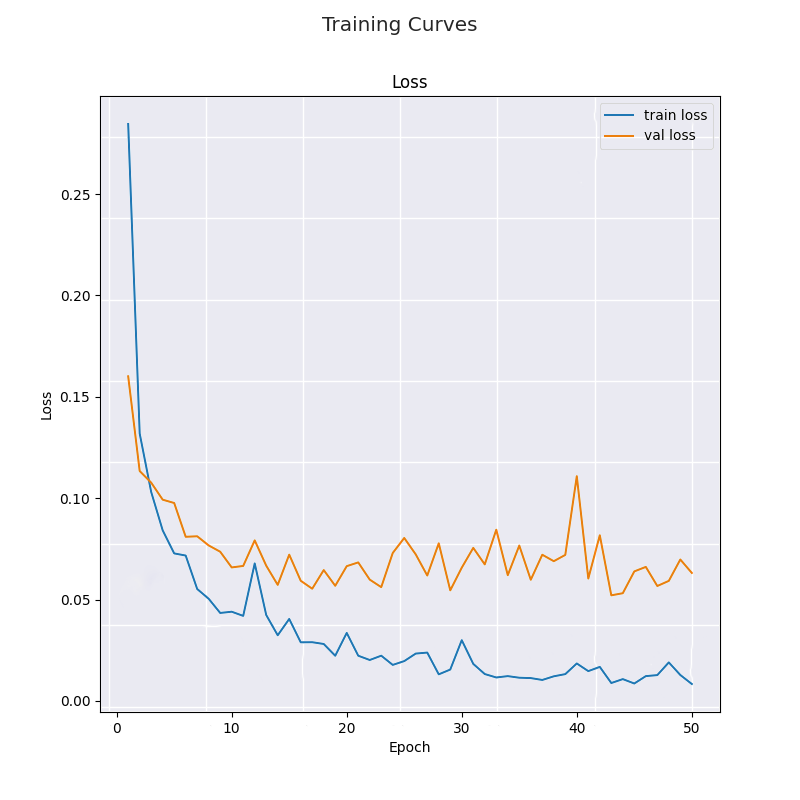
\includegraphics[ width=0.8\textwidth]{images/chapter experiments/method 4/loss.png}
    \caption{Σφάλμα εκπαίδευσης και ελέγχου μεθόδου 4 στο σύνολο \en{MNIST}.}
    \label{fig:method4}
\end{figure}

Η μη ικανοποιητική επίδοση του παρόντος αλγορίθμου, σε ένα βαθμό υποδεικνύει τη χρησιμότητα των βασικών υποθέσεων των νευρωνικών δικτύων με κάψουλες. Για παράδειγμα, η πολύ κακή επίδοση που εμφανίζεται στο σύνολο δεδομένων \en{Multi-MNIST} μας προδιαθέτει να πιστεύουμε ότι οι περισσότεροι περιορισμοί που εισάγει η τεχνολογία με την οποία καταπιάνεται ο παρόν τόμος οδηγούν σε καλύτερη ταξινόμηση των επικαλυπτώμενων ψηφίων.\par

Τέλος, να αναφέρουμε ότι η πιο τολμηρή υπόθεση που έγινε από την τέταρτη μέθοδο είναι αυτή της ενθυλάκωσης - ανεξάρτητων από το στιγμιότυπο της κλάσης - χαρακτηριστικών. Μέσα από τα πειράματα αποδείχθηκε ότι κάτι τέτοιο είναι απαραίτητο για την ορθή λειτουργία του νευρωνικού δικτύου. Επιδιώξαμε να αναιρέσουμε αυτή την υπόθεση στην τέταρτη μέθοδο και να εφαρμόζουμε τον αλγόριθμο \en{SOM} σε κάθε εικόνα εισόδου ξεχωριστά. Παρόλα αυτά, το μεγάλο υπολογιστικό κόστος του αλγορίθμου \en{SOM} κατέστησε την μέθοδο μη αποδοτική, γεγονός το οποίο ξέφευγε από τους σκοπούς της παρούσας διπλωματικής εργασίας.

\section{Σύγκριση Πειραματικών Αποτελεσμάτων Μεθόδων}

Έχωντας ολοκληρώσει όλα τα πειράματα για την κάθε μέθοδο ξεχωριστά και έχοντας συγκρίνει τους αλγορίθμους της κάθε μεθόδου μεταξύ τους, είμαστε πλέον σε θέση να συγκρίνουμε τους καλύτερους δικούς μας αλγορίθμους με αυτούς που βρίσκονται στη διεθνή βιβλιογραφία και εμφανίζουν την καλύτερη επίδοση την στιγμή της συγγραφής του έργου. Δεδομένου ότι ασχολούμαστε με μια ειδική κατηγορία τεχνητών νευρωνικών δικτύων με συγκεκριμένες ιδιότητες, θα γίνει σύγκριση και με τις πιο αξιόλογες υλοποιήσεις της εν λόγω τεχνολογίας.\par

Σε κάθε υποενότητα, πραγματοποιούμε τη σύγκριση σε καθένα πρόβλημα ξεχωριστά. Ο τρόπος με τον οποίο παρουσιάζουμε τα αποτελέσματα είναι ο εξής: 
\begin{enumerate}
    \item Στην ανώτερη βαθμίδα παρουσιάζονται τα αποτελέσματα των δικών μας αλγορίθμων.
    \item Στην δεύτερη βαθμίδα παρουσιάζονται τα αποτελέσματα των \textquote{βασικών} αλγορίθμων από την ομάδα του \en{Hinton} αλλά και αυτά που αφορούν το έργο \cite{mazzia2021efficient} από το οποίο εμπνεύστηκε η μέθοδος 3.
    \item Στην τρίτη βαθμίδα καταγράφονται οι επιδόσεις άλλων υλοποιήσεων των νευρωνικών δικτύων από κάψουλες που βρίσκονται στην βιβλιογραφία.
    \item Τέλος, στην κατώτερη βαθμίδα παρουσιάζεται το μοντέλο με την καλύτερη επίδοση για το συγκεκριμένο \en{dataset}.\par
\end{enumerate}

Προτού ξεκινήσουμε την ανάλυση για κάθε σύνολο δεδομένων ξεχωριστά, είναι σημαντικό να επαναλάβουμε ότι αν εξαιρέσουμε την τρίτη μέθοδο (και ως ένα βαθμό την τέταρτη) οι υπόλοιπες από τις μεθόδους μας δεν έχουν σκοπό την επίτευξη καλύτερης επίδοσης αλλά την διευκόλυνση στην κατανόηση του τρόπου λειτουργίας των νευρωνικών δικτύων με κάψουλες. Επίσης, διευκολύνουν στην σύγκριση με τις μεθόδους μας αφού μέσα από τον πειραματισμό τους αποκτήσαμε χρήσιμες μετρικές που ήταν αδύνατο να αποκομιστούν διαφορετικά. Ακόμα, για τις μεθόδους που προτείνουμε εμείς, τόσο η αναζήτηση στον χώρο παραμέτρων όσο και η εκπαίδευση (από πλευράς χρόνου) δεν είναι πλήρεις και καλύτερες επιδόσεις μπορούν να προκύψουν με μια πιο εκτενή πειραματική μελέτη. \par




\subsection{Σύνολο Δεδομένων \en{SmallNORB}}
Το σύνολο δεδομένων \en{SmallNORB} αποτελεί μια χαρακτηριστική δοκιμασία για τα νευρωνικά δίκτυα με κάψουλες αφού μέσω αυτού δοκιμάζεται η ικανότητά τους για αναγνώριση αντικειμένων από διαφορετικές οπτικές γωνίες. Ας μην ξεχνάμε ότι η αποδοτική αναγνώριση τέτοιων εικόνων είναι πρωταρχικός στόχος της συγκεκριμένης τεχνολογίας.\par

Ο αριθμός των παραμέτρων δεν μαρτυρά πάντα την υπολογιστική πολυπλοκότητα του δικτύου, ειδικά στην περίπτωσή μας όπου χρησιμοποιούνται επαναληπτικοί αλγόριθμοι δρομολόγησης. Για τον σκοπό αυτό, ειδικά για το συγκεκριμένο πρόβλημα κάναμε επιπλέον μετρήσεις του αριθμού των πράξεων κινητής υποδιαστολής που πραγματοποιούνται το δευτερόλεπτο, για ένα \en{batch} μεγέθους 1. Για να μετριάσουμε την υπολογιστική επιβάρυνση που προστίθεται κατά την αρχικοποίηση των μητρώων (\en{tensors}), όλες οι μετρήσεις έγιναν για μέγεθος δέσμης ίσο με 8 και το αποτέλεσμα το διαιρούμε με το 8 για να λάβουμε την τιμή \en{FLOPs per 1 batch}. Προφανώς, επειδή οι μετρήσεις μας αφορούν το κόστος πρόβλεψης (\en{inference}), στις μετρήσεις δεν περιλαμβάνεται το υπολογιστικό κόστος του αποκωδικοποιητή (όπου χρησιμοποιείται).\par

Στον πίνακα \ref{tab:all_methods_comparison_smallnorb} παρουσιάζονται οι επιδόσεις τόσο των δικών μας μεθόδων όσο και μεθόδων που συναντώνται στην βιβλιογραφία. Στη τελευταία βαθμίδα παρουσιάζεται το έργο με την καλύτερη επίδοση. Αν τυχαίνει να είναι και νευρωνικό δίκτυο με κάψουλες (όπως στην περίπτωσή μας), θα εμφανίζεται δύο φορές στην λίστα (μια επιπλέον στην τρίτη βαθμίδα όπου παρατίθενται οι επιδόσεις των \en{Capsule Networks} της βιβλιογραφίας).

\begin{table}[h]
    \begin{center}
        \en{
        \begin{tabular}{c c c c c}
            \toprule
            Algorithm (Method) & Recon. & Parameters (K) & $FLOPs|_{1 batch}$ (\en{G}) & SmallNORB (\%) \\ 
            \midrule
            Argmax Scaled (1)  & yes & 6816 & 0.705 & 16.49 \\
            Multi-Head RoMAV (3)  & yes & 152.8 &  0.0473 &  \textbf{1.44} \\
            Multi-Head RoMAV (3)  & no & 152.8 &  0.0473 &  1.58 \\
            SOM-Based Var.1 (4) & no & 670.5 & 0.889 & 5.30\\
            Our Dynamic (1) & yes & $6800$ & $0.7$ & 17.01\\
            Our EM-Routing (2) & no & $310$ & $0.675$  & 14.04\\
            \midrule
            Dynamic \cite{sabour2017dynamic} & yes & $6800$ & $0.7$ & 2.7\\
            EM-Routing \cite{hinton2018matrix} & no & $310$ & $0.675$  & \textbf{1.8}\\
            Efficient-CapsNet \cite{mazzia2021efficient} & yes & 151 & 0.06 & 2.54\\
            \midrule
            VB-Routing \cite{De_Sousa_Ribeiro_Leontidis_Kollias_2020_Capsule_Routing} & no & 169 & - & 1.6\\
            RU-Routing \cite{de2020introducing} & no & 140 & - & 1.4\\
            DC-Net \cite{phaye2018dense} & yes & 11800 & - & 5.57\\
            DC-Net++ \cite{phaye2018dense} & yes & 11800 & - & 4.66\\
            FREM \cite{zhang2018fast} & no & 1200 & - & 2.2\\
            FRMS \cite{zhang2018fast} & no & 1200 & - & 2.6\\
            STAR-Caps \cite{NEURIPS2019_cf040fc7_star_caps} & no & 318 & - & 1.8\\
            Heinsen Routing\cite{heinsen2019algorithm} & no & 272 & - & \textbf{0.9}\\
            \midrule % Best
            Heinsen Routing\cite{heinsen2019algorithm} & no & 272 & - & \textbf{0.9}\\
            \bottomrule
        \end{tabular}
        }
    \end{center}
    \caption[]{\label{tab:all_methods_comparison_smallnorb}Σύγκριση της επίδοσης των μεθόδων μας με αυτές στην βιβλιογραφία για το σύνολο δεδομένων \en{SmallNORB}.} 
\end{table}

Τα αποτελέσματα των μεθόδων μας είναι πλήρως ικανοποιητικά, αν εξαιρέσουμε την τέταρτη μέθοδο. Ο αλγόριθμος \en{Argmax Scaled} της πρώτης μεθόδου μπορεί να μην εμφανίζει καλά αποτελέσματα αλλά πρέπει να λάβουμε υπόψη ότι δεν έγινε καμία ειδική αναζήτηση υπερπαραμέτρων για το συγκεκριμένο σύνολο δεδομένων στην πρώτη μέθοδο. Συνεπώς, το γεγονός ότι έχει καλύτερη επίδοση από την δική μας υλοποίηση του αλγορίθμου του έργου \cite{sabour2017dynamic} όταν οι δύο εκπαιδεύτηκαν υπό τις ίδιες συνθήκες ενδέχεται να σημαίνει ότι τελικά, μπορεί να εμφανίζει καλύτερη επίδοση.\par

Την μεγαλύτερη επιτυχία την σημειώνει η τρίτη μέθοδος η οποία μετά από εκπαίδευση σε μόλις 30 εποχές και χωρίς ιδιαίτερα αντίμετρα υπερπροσαρμογής, ανταγωνίζεται τις καλύτερες μεθόδους της βιβλιογραφίας (τρίτη σε σειρά επίδοσης). Η επίδοση \en{1.44} (20.0\% μείωση ποσοστιαίου σφάλματος σε σχέση με τον \en{EM}) επιτυγχάνεται με λιγότερο από το ένα δέκατο της υπολογιστικής πολυπλοκότητας (93\% βελτίωση) και τις μισές παραμέτρους. Ακόμα και χωρίς ανακατασκευαστή, οι επιδόσεις είναι πολύ υψηλές, γνωρίζοντας μάλιστα ότι η μέθοδος επιδέχεται περαιτέρω βελτίωση. Αν και στοιχεία υπολογιστικής πολυπλοκότητας απουσιάζουν για τις περισσότερες μεθόδους, η μη επαναληπτική φύση του αλγορίθμου μας οδηγεί να πιστεύουμε ότι ο αλγόριθμος \en{Multi-Head RoMAV} της τρίτης μεθόδου είναι αυτός με την καλύτερη σχέση επίδοσης\textendash ταχύτητας στην βιβλιογραφία στο συγκεκριμένο πρόβλημα. Τέλος, εφιστούμε την προσοχή στο αποτέλεσμα της μεθόδου \en{Efficient-CapsNet} \cite{mazzia2021efficient} που χρησιμοποιεί τον \textquote{απλοικό αλγόριθμο προσοχής} της μεθόδου 3 (αλγόριθμος \ref{alg:method3_stupid_routing}). Βλέπουμε ότι με σχεδόν τις ίδιες παραμέτρους και πράξεις κινητής υποδιαστολής επιτυγχάνουμε πολύ υψηλότερα αποτελέσματα χρησιμοποιώντας αλγορίθμους με πολύ καλύτερη ποιοτική ερμηνεία.

\subsection{Σύνολο Δεδομένων \en{MNIST}}

Το συγκεκριμένο σύνολο αποτελεί ένα από τα ευκολότερα σύνολα δεδομένων για τα σημερινά νευρωνικά δίκτυα και το πρόβλημα είναι σε μεγάλο βαθμό \textquote{λυμένο}. Ο ρόλος του στα νευρωνικά δίκτυα με κάψουλες είναι κυρίως στο να αποδείξουν ότι μπορούν να αποδομήσουν τα ψηφία στις παραμέτρους στιγμιοτύπου τους. Επίσης, χρησιμοποιείται ως βάση σε άλλα σύνολα δεδομένων όπως το \en{affNIST} και το \en{MultiMNIST}. Τα σχετικά πειράματα παρουσιάζονται στον πίνακα \ref{tab:all_methods_comparison_mnist}.

\begin{table}[h]
    \begin{center}
        \en{
        \begin{tabular}{c c c c}
            \toprule
            Algorithm (Method) & Recon. & Parameters (K) & MNIST (\%) \\ 
            \midrule
            Argmax Scaled (1)  & yes & 6816  & 0.37 \\
            Multi-Head RoMAV (3)  & yes & 162.7 & \textbf{0.3} \\
            Multi-Head RoWLS (3)  & no & 162.7 &  0.34 \\
            SOM-Based Var.3 (4) & no & 670 & 0.52 \\
            Our Dynamic (1) & yes & 6800 &  0.31\\
            \midrule
            Dynamic \cite{sabour2017dynamic} & yes &  6800 & 0.25\\
            Dynamic \cite{sabour2017dynamic} & no &  6800 & 0.35\\
            EM-Routing \cite{hinton2018matrix} & no & 310  & 0.44\\
            Efficient-CapsNet \cite{mazzia2021efficient} & yes & 161 & \textbf{0.26}\\
            \midrule
            VB-Routing \cite{De_Sousa_Ribeiro_Leontidis_Kollias_2020_Capsule_Routing} & no & 169 & 0.3\\
            RU-Routing \cite{de2020introducing} & no & > 440 &  \textbf{0.28}\\
            DC-Net \cite{phaye2018dense} & yes & 11800 &  0.28 \\
            DC-Net++ \cite{phaye2018dense} & yes & 11800 &  0.29 \\
            FREM \cite{zhang2018fast} & no & 1200 & 0.38\\
            % FRMS \cite{zhang2018fast} & no & 1200 &  - \\
            STAR-Caps \cite{NEURIPS2019_cf040fc7_star_caps} & no & 281 & 0.43\\
            DA-CapsNet \cite{huang2020capsnet} & yes & 7000 & 0.47\\
            HitNet \cite{deliege2018_hitnet}& yes& >= 8000 &0.32\\
            Nair \cite{nair2021pushing_Nair}& no & 8200 & 0.5\\
            DeepCaps \cite{rajasegaran2019deepcaps}& yes & 7220 & 0.28\\

            \midrule % Best
            CNN Ensemble \cite{an2020ensemble} & no & $\infty$ & \textbf{0.09}\\
            \bottomrule
        \end{tabular}
        }
    \end{center}
    \caption[]{\label{tab:all_methods_comparison_mnist}Σύγκριση της επίδοσης των μεθόδων μας με αυτές στην βιβλιογραφία για το σύνολο δεδομένων \en{MNIST}.} 
\end{table}

Στο πρόβλημα \en{MNIST} ο αλγόριθμος με την καλύτερη επίδοση είναι πάλι ο \en{Multi-Head RoMAV} της τρίτης μεθόδου. Το υψηλό αποτέλεσμα είναι ιδιαίτερα αξιόλογο αν αναλογιστεί κανείς ότι δεν έγινε καμία αναζήτηση υπερπαραμέτρων για το συγκεκριμένο πρόβλημα και ότι η εκπαίδευση έγινε μόλις για 30 εποχές. Συνεπώς, παρατηρούμε ότι υπό την ίδια παραμετροποίηση ο ίδιος αλγόριθμος που πετυχαίνει ανταγωνιστικά για τη βιβλιογραφία αποτελέσματα στο σύνολο \en{SmallNORB} έχει πολύ καλές επιδόσεις και στο σύνολο \en{MNIST}\footnote{Με μικρές διαφορές στην αρχιτεκτονική των πρώτων επιπέδων η οποία τώρα δεν περιέχει επίπεδα \en{Instance Normalization}.}. Είναι σημαντικό να αναφέρουμε ότι σχεδόν όλοι οι αλγόριθμοι της βιβλιογραφίας με καλύτερη επίδοση δεν αποδεικνύουν την αποδόμηση των εικόνων του συνόλου δεδομένων σε ισομεταβλητές παραμέτρους (\en{equivariant parameters}) όπως εμείς κάναμε. Επιπλέον, προσθέτουμε ότι από στοιχεία που αποκτήσαμε κατά την διάρκεια της εκπαίδευσης, πιστεύουμε ότι η επίδοση μπορεί να βελτιωθεί περαιτέρω. Τέλος, σημειώνουμε ότι σε σχέση με την καλύτερη υλοποίηση από τα βασικά έργα (\cite{kosiorek2019stacked,sabour2017dynamic,hinton2018matrix}) χωρίς ανακατασκευαστή επιτυγχάνονται καλύτερα αποτελέσματα.\par

\subsection{Σύνολο Δεδομένων \en{CIFAR10}}
Πρόκειται για το πιο σύνθετο σύνολο δεδομένων. Είναι σύνηθες τα νευρωνικά δίκτυα με κάψουλες να μην έχουν υψηλή επίδοση σε αυτό. Τα σχετικά αποτελέσματα παρουσιάζονται στον πίνακα \ref{tab:all_methods_comparison_cifar10}.

\begin{table}[h]
    \begin{center}
        \en{
        \begin{tabular}{c c c c}
            \toprule
            Algorithm (Method) & Recon. & Parameters (K) & CIFAR10 (\%) \\ 
            \midrule
            Argmax Scaled (1)  & yes & 7000  & 22.16 \\
            Multi-Head RoMAV (3)  & yes & 265.2  & 28.85 \\
            Multi-Head RoMAV (3)  & no & 265.2  &  29.74 \\
            SOM-Based Var.2 (4) & no & 670 & 34.555 \\
            Our Dynamic (1) & yes & 7000 &  \textbf{21.64}\\
            \midrule
            Dynamic \cite{sabour2017dynamic} & yes &  6800 & \textbf{10.6}\\
            EM-Routing \cite{hinton2018matrix} & no & 460  & 11.9\\
            % Efficient-CapsNet \cite{mazzia2021efficient} & yes & 161 & - \\
            \midrule
            VB-Routing \cite{De_Sousa_Ribeiro_Leontidis_Kollias_2020_Capsule_Routing} & no & 323 & 11.2\\
            % RU-Routing \cite{de2020introducing} & no & > 440 &  -\\
            DC-Net \cite{phaye2018dense} & yes & 11800 & 17.37 \\
            DC-Net++ \cite{phaye2018dense} & yes & 11800 &  10.29 \\
            FREM \cite{zhang2018fast} & no & 1200 & 14.3\\
            FRMS \cite{zhang2018fast} & no & 1200 &  15.6 \\
            STAR-Caps \cite{NEURIPS2019_cf040fc7_star_caps} & no & 281 & \textbf{8.77}\\
            DA-CapsNet \cite{huang2020capsnet} & yes & 7000 & 14.53\\
            HitNet \cite{deliege2018_hitnet}& yes& >= 8000 &26.70 \\
            Nair \cite{nair2021pushing_Nair}& no & 8200 & 32.47\\
            DeepCaps \cite{rajasegaran2019deepcaps}& yes & 7220 & 8.99\\
            \midrule % Best
            ViT-H/14 \cite{dosovitskiy2020image_is_worth_16} & no & $\infty$ & \textbf{0.5}\\
            \bottomrule
        \end{tabular}
        }
    \end{center}
    \caption[]{\label{tab:all_methods_comparison_cifar10}Σύγκριση της επίδοσης των μεθόδων μας με αυτές στην βιβλιογραφία για το σύνολο δεδομένων \en{CIFAR10}.} 
\end{table}

Στο συγκεκριμένο σύνολο, οι επιδόσεις μας είναι χειρότερες από τις περισσότερες της βιβλιογραφίας. Αυτό πιθανότατα οφείλεται αφενός στον μικρό αριθμό εποχών και αφετέρου στον χαμηλό αριθμό παραμέτρων που έχουμε (για τις μεθόδους 3 και 4). Φυσικά, επειδή για τους αλγορίθμους της μεθόδου 3, δεν έγινε καμία αναζήτηση υπερπαραμέτρων, η επίδοση πιθανότατα επιδέχεται βελτίωση.

\subsection{Σύνολο Δεδομένων \en{MultiMNIST}}

Για το σύνολο αυτό, δεν υπάρχουν αρκετές μέθοδοι με τις οποίες μπορεί να συγκριθεί. Η δυσκολεία υλοποίησης του συγκεκριμένου προβλήματος έχει αποτρέψει πολλούς ερευνητές στον να δοκιμάσουν το έργο τους σε αυτό. Τα πειράματα για το σύνολο αυτό και η σύγκρισή τους εμφανίζοντια στον πίνακα \ref{tab:all_methods_comparison_multimnist}. Όπως και για το σύνολο \en{SmallNORB}, η μέθοδος με την καλύτερη επίδοση είναι μια μέθοδος νευρωνικών δικτύων με κάψουλες.

\begin{table}[h]
    \begin{center}
        \en{
        \begin{tabular}{c c c}
            \toprule
            Algorithm (Method) & Recon. & MultiMNIST (\%) \\ 
            \midrule
            Argmax Scaled (1)  & yes  & - \\
            Multi-Head RoMAV (3)  & yes   & \textbf{6.2115} \\
            Multi-Head RoMAV (3)  & no   &  6.2615 \\
            SOM-Based Var.3 (4) & no & 22.954 \\
            % Our Dynamic (1) & yes &  - \\
            \midrule
            Dynamic \cite{sabour2017dynamic} & yes & \textbf{5.0}\\
            % EM-Routing \cite{hinton2018matrix} & no   & -\\
            % Efficient-CapsNet \cite{mazzia2021efficient} & yes  & - \\
            \midrule
            % VB-Routing \cite{De_Sousa_Ribeiro_Leontidis_Kollias_2020_Capsule_Routing} & no & -\\
            RU-Routing \cite{de2020introducing} & no &  \textbf{1.8}\\
            % DC-Net \cite{phaye2018dense} & yes  & - \\
            % DC-Net++ \cite{phaye2018dense} & yes  &  - \\
            % FREM \cite{zhang2018fast} & no  & -\\
            % FRMS \cite{zhang2018fast} & no  &  - \\
            % STAR-Caps \cite{NEURIPS2019_cf040fc7_star_caps} & no & -\\
            % DA-CapsNet \cite{huang2020capsnet} & yes  & -\\
            % HitNet \cite{deliege2018_hitnet}& yes &- \\
            % Nair \cite{nair2021pushing_Nair}& no  & -\\
            % DeepCaps \cite{rajasegaran2019deepcaps}& yes & -\\
            Aff-Caps \cite{aff_Caps_Gu} & no & 4.51\\
            Aff-Caps \cite{aff_Caps_Gu} & yes & 5\\
            \midrule % Best
            RU-Routing \cite{de2020introducing} & no &  \textbf{1.8}\\
            \bottomrule
        \end{tabular}
        }
    \end{center}
    \caption[]{\label{tab:all_methods_comparison_multimnist}Σύγκριση της επίδοσης των μεθόδων μας με αυτές στην βιβλιογραφία για το σύνολο δεδομένων \en{MultiMNIST}.} 
\end{table}

Δοκιμάσαμε τις νέες μεθόδους που προτείνουμε (3 και 4) στο \en{MultiMNIST} και τα αποτελέσματα είναι πολύ διαφωτιστικά. Βλέπουμε ότι η μέθοδος 4 που απέχει αρκετά από τις θεμελιώδεις υποθέσεις των νευρωνικών δικτύων με κάψουλες αποτυγχάνει στο συγκεκριμένο σύνολο. Στον αντίποδα βρίσκεται η μέθοδος 3 η οποία έχει εξαιρετικά αποτελέσματα δεδομένου ότι δεν έγινε καμία αναζήτηση υπερπαραμέτρων και καμία προσαρμογή της αρχιτεκτονικής του δικτύου σε αυτό το ιδιαίτερο σύνολο δεδομένων. Είμαστε βέβαιοι ότι με την χρήση καλύτερου αποκωδικοποιητή και περισσότερων εποχών τα αποτελέσματα της τρίτης μεθόδου θα βελτιωθούν\footnote{Παρατηρήσαμε πως κατά την εκπαίδευση σε 30 εποχές το σφάλμα ελέγχου είχε συνεχώς καθοδική τάση. Δυστυχώς, περιορισμοί χρονικοί και υλικού δεν μας επέτρεψαν τον εκτενή πειραματισμό των 6 αλγορίθμων της μεθόδου 3 στο συγκεκριμένο σύνολο.}

\subsection{Σύνολο Δεδομένων \en{FashionMNIST}}

Το σύνολο \en{FashionMNIST} αποτελεί μια πιο σύνθετη εκδοχή του \en{MNIST} και στα πειράματα σκοπό έχει να δοκιμάσει κυρίως την ικανότητα των νευρωνικών δικτύων με κάψουλες για αναγνώριση αντικειμένων υπό διαφορετικά στυλ. Αυτό διότι οι εικόνες που περιέχει είναι εικόνες \textquote{πρόσοψης} και δεν έχουν ληφθεί από διαφορετικές οπτικές γωνίες. Στον πίνακα \ref{tab:all_methods_comparison_fashionmnist} συγκεντώνονται τα αποτελέσματα των πειραμάτων μας αλλά και αυτά της βιβλιογραφίας. Όπως πάντα, στην τελευταία βαθμίδα έχουμε την καλύτερη μέθοδο της βιβλιογραφίας που στην περίπτωσή μας, δεν είναι νευρωνικό δίκτυο από κάψουλες.
\begin{table}[h]
    \begin{center}
        \en{
        \begin{tabular}{c c c}
            \toprule
            Algorithm (Method) & Recon. & FashionMNIST (\%) \\ 
            \midrule
            Argmax Scaled (1)  & yes  & 7.00 \\
            Multi-Head RoMAV (3)  & yes  & 8.22 \\
            Multi-Head RoMAV (3)  & no   &  7.84 \\
            SOM-Based Var.3 (4) & no  & 9.51 \\
            Our Dynamic (1) & yes &  \textbf{6.94}\\
            \midrule
            %Dynamic \cite{sabour2017dynamic} & yes & -\\
            %EM-Routing \cite{hinton2018matrix} & no   & -\\
            %Efficient-CapsNet \cite{mazzia2021efficient} & yes  & - \\
            - & -  & - \\
            \midrule
            VB-Routing \cite{De_Sousa_Ribeiro_Leontidis_Kollias_2020_Capsule_Routing} & no & \textbf{5.2}\\
            %RU-Routing \cite{de2020introducing} & no &  -\\
            DC-Net \cite{phaye2018dense} & yes  & 5.36 \\
            DC-Net++ \cite{phaye2018dense} & yes  &  5.35 \\
            FREM \cite{zhang2018fast} & no  & 6.2\\
            FRMS \cite{zhang2018fast} & no  &  6.0 \\
            %STAR-Caps \cite{NEURIPS2019_cf040fc7_star_caps} & no & -\\
            DA-CapsNet \cite{huang2020capsnet} & yes  & 6.02\\
            HitNet \cite{deliege2018_hitnet}& yes &7.7 \\
            Nair \cite{nair2021pushing_Nair}& no  & 10.2\\
            DeepCaps \cite{rajasegaran2019deepcaps}& yes & 5.54\\
            \midrule % Best
            Fine-Tuning DARTS\cite{tanveer2021fine} & no  & \textbf{3.09}\\
            \bottomrule
        \end{tabular}
        }
    \end{center}
    \caption[]{\label{tab:all_methods_comparison_fashionmnist}Σύγκριση της επίδοσης των μεθόδων μας με αυτές στην βιβλιογραφία για το σύνολο δεδομένων \en{FashionMNIST}.} 
\end{table}

Και πάλι, οι λίγες εποχές που χρησιμοποιούνται σε συνδυασμό με τον μειωμένο αριθμό παραμέτρων οδηγούν σε χαμηλότερη επίδοση (υψηλότερο ποσοστό σφάλματος) σε σχέση με πολλές μεθόδους της βιβλιογραφίας. Επίσης, η έντονη επαύξηση των δεδομένων (με περιστροφή) που χρησιμοποιούμε στο συγκεκριμένο σύνολο δεδομένων (για τις μεθόδους 3 και 4) δεν διευκολύνει την επίδοση. Ειδικά για την τρίτη μέθοδο, το γεγονός ότι η προσθήκη ανακατασκευαστή επιδεινώνει το ποσοστιαίο σφάλμα μας προδιαθέτει στο να πιστέψουμε ότι καλύτερη αναζήτηση υπερπαραμέτρων θα προσφέρει υψηλότερη ακρίβεια.
\enlargethispage{\baselineskip}
% Για κάθε dataset ξεχωριστά. Όχι νέα πειράματα.